\documentclass[a4paper, titlepage]{jsreport} 
\usepackage{amsmath, amssymb, amsfonts, color, bm}
\usepackage[dvipdfmx]{graphicx}
\setcounter{tocdepth}{3}
\title{Twisted Landau-Zener遷移を含む周期的な量子系における\\幾何学的効果\\
Geometric Effects in Cyclic Evolution \\with Twisted Landau-Zener Transition}

\author{非公開}
\date{\today}
\begin{document} 
\maketitle
\tableofcontents
\newpage
\chapter{はじめに}

\section{研究背景および本論文の目的}

Berryは周期系における波動関数の位相に,自明でない幾何学的な項が含まれることを指摘した\cite{Berry1984}.この項はBerry位相として広く知られている.Berryの指摘から40年が経過した現在,Berry位相は固体物理学や量子操作などの幅広い分野で欠かせない概念である.


また,非断熱遷移は自然界で広く見られる現象である.特に,Landau-Zenerモデルは非断熱遷移のもっとも簡単な例であるにもかかわらず,原子の非弾性衝突や磁場中の粒子のスピン遷移などの数多くの現象を説明することができる\cite{Zener}.それに加えて,Landau-Zenerモデルに干渉効果を取り入れたモデルでは,強め合う干渉や弱め合う干渉によって状態の占有確率を制御することができる\cite{Kayanuma1993}.


さらに,非断熱遷移では,ある種の幾何学量が遷移確率に影響を与える場合がある\cite{Berry1990}.Twisted Landau-Zenerモデルがその代表例である.このモデルでは,パラメータ空間における測地曲率を調整することによって,遷移確率の制御が可能になる\cite{Oka}.特に,トンネル確率が100%になる完全トンネルを実現できる点は重要である.


これらの研究は,現在まで独立に行われてきた背景がある.そのため,これらの概念が複雑に絡みあった現象を扱うことができない.実際の自然界で起こる現象をより正確に議論するためには,上で挙げたモデルを組み合わせた新しいモデルによる一般化が求められる.


以上を踏まえて,本研究では,Twisted Landau-Zenerモデルを複数回繰り返すモデルを新たに考案し,波動関数の干渉と測地曲率が引き起こす現象に注目する.特に,これら2つの要因によって,特有の動力学が見られることを示す.

\section{本論文の構成}
本節では,本論文における各章の概要を説明する.


第2章では,量子力学における断熱遷移を説明する.また,最終的には,Berry位相という概念を,Berryが用いた方法に準じて説明することが本章の目標である.そのため,Berry位相の説明に必要な概念を事前に定義しておくことで,量子力学の前提知識をなるべく要求しないことを心掛けた.


第3章では,量子力学における非断熱遷移を説明する.特に,非断熱遷移では,幾何学的な量が重要な役割を担うことを強調する.はじめに,ある種の幾何学的位相が非断熱遷移の確率に影響を与えることを,一般的なHamiltonianを用いて示す.その後,Landau-ZenerモデルやTwisted Landau-Zenerモデルという,非断熱遷移の具体的な例を提示する.


第4章では,cyclic evolutionについて解説する.特に,本論文のメインテーマである,Twisted Landau-Zener遷移を含むcyclic evolutionを理解するために必要な知識に重点を置く.


第5章では,本論文のメインテーマであるTwisted Landau-Zener遷移を含むcyclic evolutionについて説明し,波動関数の干渉と測地曲率が織りなす現象について,数値計算の結果を踏まえて考察する.


第6章では,本論文のまとめを示し,今後の展望について説明する.


付録では,構成の都合上,本文では割愛したが,本論文の内容をさらに深く理解するために重要な事柄を説明する.具体的には,Landau-Zener公式\cite{Zener}およびDykhne-Davis-Pechukas法\cite{Dykhne}\cite{DavisPechukas1976}\cite{Hwang}の証明を行う.
\section{本論文で用いられる記法}
以下の記法は,本文で特に断りなく用いることにする.\\
\begin{itemize} 
  \item
    「$A$は$B$によって定義される」ということを,
    \begin{equation}
      A := B
    \end{equation}
    で表す.
  \item
    ある変数$x$についての偏微分を,
    \begin{equation}
      \partial_x := \frac{\partial}{\partial x}
    \end{equation}
    と書くことがある.
  \item 実数全体の集合を$\mathbb{R}$,複素数全体の集合を$\mathbb{C}$とする.
  \item $\hbar$は,Dirac定数(換算Planck定数)である.これは,Planck定数を$2\pi$で割った値である.
  \item 以下の3つの$2\times2$行列
\begin{equation}
  \Hat{\sigma}_x=
  \begin{pmatrix}
    0 & 1\\
    1 & 0\\
  \end{pmatrix}
  ,
  \Hat{\sigma}_y=
  \begin{pmatrix}
    0 & -i\\
    i & 0\\
  \end{pmatrix}
  ,
  \Hat{\sigma}_z=
  \begin{pmatrix}
    1 & 0\\
    0 & -1\\
  \end{pmatrix}
\end{equation}
はPauli行列である.また,各Pauli行列$\Hat{\sigma}_i (i = x,y,z)$をベクトルの成分とみなして,
\begin{equation}
  \bm{\Hat{\sigma}} = (\Hat{\sigma}_x, \Hat{\sigma}_y, \Hat{\sigma}_z)
\end{equation}
と書くことがある.
\end{itemize}

\chapter{断熱遷移} \label{AT}
本章では,量子力学における断熱遷移に関連する内容を説明する.

\section{断熱状態}
$N$準位系($N$-level system)のHamiltonianを$\Hat{H}(t)$,状態ベクトル(state vector)を$|\psi(t)\rangle$とすると,状態ベクトルの時間発展は,Shr\"{o}dinger方程式
\begin{equation}
  \label{SE}
  i\hbar \frac{d}{dt} |\psi(t) \rangle = \Hat{H}(t) |\psi(t) \rangle
\end{equation}
で与えられる.
また,各時刻$t$において,固有値方程式
\begin{equation} 
  \Hat{H}(t) |\phi_n(t) \rangle = E_n(t) |\phi_n(t) \rangle \quad (n = 1,\,2,\,\ldots,\,N) \label{EE}
\end{equation}
が成立する.ここで,$\Hat{H}(t)$の固有値$E_n(t)$を断熱エネルギー(adiabatic energy)あるいは瞬間エネルギー(instantaneous energy)と呼ぶ.また,それぞれの固有値に属する規格直交化された固有ベクトル$|\phi_n(t) \rangle$を断熱状態(adiabatic state)と呼ぶ.ただし,属する固有値が小さい順に添え字$n$をつける.


断熱状態の組$\{|\phi_n(t) \rangle\}_{n=1}^N$は,完全系をなすことが知られている.この組を断熱基底(adiabatic base)と呼ぶ.断熱基底を用いると,系の状態ベクトル$|\psi(t)\rangle$は.
\begin{equation}
  |\psi(t) \rangle = \sum_{n=1}^{N} c_n(t) |\phi_n(t)\rangle  \quad (c_n(t) \in \mathbb{C})
\end{equation}
で表される.
\section{伝統的な断熱定理}
$N$準位系が時刻$t_0$から$t_0+\Delta t$まで時間発展するとき,
\begin{equation} \label{AT1}
  \left| \langle E_m(t) | \Dot{E}_n(t) \rangle \right| \ll \left| \omega_{nm}(t) \right| \quad (m\ne n)
\end{equation}
あるいは,
\begin{equation} \label{AT2}
  \max_{t\in [t_0, t_0+\Delta t]} \frac{\left| \langle E_m(t) |\Dot{\Hat{H}}(t)| E_n(t) \rangle \right|}{\omega_{nm}(t)^2} \ll 1 \quad (m\ne n)
\end{equation}
を(伝統的な)断熱条件(adiabatic condition)と呼ぶ\footnote{式(\ref{AT1})と式(\ref{AT2})が等価であることは,式(\ref{EE})を微分して式(\ref{AT1})に代入することで容易に確かめられる.}.ただし,$\omega_{nm} := \hbar^{-1} \left( E_n(t)-E_m(t) \right)$である.系が断熱条件を満たすとき,$|c_n|^2$の比(各状態の占有確率)は変化しない.これを断熱定理(adiabatic theorem)と呼ぶ.また,断熱定理にしたがった遷移を断熱遷移(adiabatic transition)と呼ぶ.

\section{新たな断熱定理}
近年,断熱条件を拡張することで,幾何学的な効果を取り入れられることが明らかになった\cite{Wu2008}.新しい断熱条件は,
\begin{equation}
  \left| \langle E_m(t) | \Dot{E}_n(t) \rangle \right| \ll \left| \omega_{nm}(t) + \Delta_{mn}(t) \right| \quad (m\ne n) 
\end{equation}
で与えられる.ここで,
\begin{equation}
  \Delta_{mn}(t) := \frac{1}{\hbar} \left\{ i \left( \langle \phi_m(t) | \Dot{\phi}_m(t) \rangle - \langle \phi_n(t) | \Dot{\phi}_n(t) \rangle \right)+ \frac{d}{dt} \arg \left( i \langle \phi_n(t) | \Dot{\phi}_m(t) \rangle \right) \right\}
\end{equation}
をquantum geometric potential(QGP)と呼ぶ.QGPは,後に説明する測地曲率と関係づけることができる.実際に,2準位系の場合について,このことを示そう.2準位系のHermiteなHamiltonianを
\begin{align}
  \Hat{H}(t)
  &= x(t)\Hat{\sigma}_x + y(t) \Hat{\sigma}_y + z(t) \Hat{\sigma}_z\\
  &=
  \begin{pmatrix} 
    z(t) & x(t) - iy(t)\\
    x(t) + iy(t) & -z(t)\\
  \end{pmatrix}\\
  &= E_2(t)
  \begin{pmatrix} 
    \cos \theta(t) & \sin \theta(t) \exp(-i\phi(t))\\
    \sin \theta(t) \exp(+i\phi(t)) & -\cos \theta(t)\\
  \end{pmatrix}
\end{align}
とする.ただし,直交座標$\{x(t), y(t), z(t)\}$から極座標$\{E_2(t), \theta(t), \phi(t)\}$への変換式
\begin{align}
  x(t) &= E_2(t) \sin \theta(t) \cos \phi(t)\\
  y(t) &= E_2(t) \sin \theta(t) \sin \phi(t)\\
  z(t) &= E_2(t) \cos \theta(t)
\end{align}
を用いた.また,$E_2(t)$は,$E_2(t) = \sqrt{x^2 + y^2 + z^2}$で表される断熱エネルギーの1つである.このとき,2つの断熱状態$|\phi_1(t) \rangle, |\phi_2(t) \rangle$は,
\begin{align}
  |\phi_1(t) \rangle
  &= 
  \begin{pmatrix}
    \sin \frac{\theta}{2}\\
    -e^{i\phi} \cos \frac{\theta}{2}
  \end{pmatrix},\\
  |\phi_2(t) \rangle
  &=
  \begin{pmatrix}
    \cos \frac{\theta}{2}\\
    e^{i\phi} \sin \frac{\theta}{2}
  \end{pmatrix}
\end{align}
であるから,これらの時間微分は,
\begin{align}
  |\Dot{\phi}_1(t) \rangle
  &= 
  \begin{pmatrix}
    -\frac{\Dot{\theta}}{2} \sin \frac{\theta}{2}\\
    -e^{i\phi} (i\Dot{\phi} \sin \frac{\theta}{2} + \frac{\Dot{\theta}}{2}\cos \frac{\theta}{2})
  \end{pmatrix},\\
  |\Dot{\phi}_2(t) \rangle
  &=
  \begin{pmatrix}
    \frac{\Dot{\theta}}{2} \cos \frac{\theta}{2}\\
    e^{i\phi} (-i\Dot{\phi} \cos \frac{\theta}{2} + \frac{\Dot{\theta}}{2}\sin \frac{\theta}{2})
  \end{pmatrix}
\end{align}
となる.したがって,
\begin{equation}
  \Delta_{mn} = \frac{\Dot{\theta} \Ddot{\phi} \sin \theta + 2 \Dot{\theta}^2 \Dot{\phi} \cos\theta + \Dot{\phi}^3 \sin^2\theta \cos \theta - \Dot{\phi} \Ddot{\theta} \sin \theta}{\Dot{\theta}^2 + (\Dot{\phi} \sin \theta)^2}
\end{equation}
である.一方,パラメータ空間の単位球表面を動く曲線における測地曲率$\kappa_g$は,位置ベクトルを$\bm{r}(t)$とすると,
\begin{align}
  \kappa_g 
  &= \left(\bm{r} \times \frac{d \bm{r}}{ds} \right) \cdot \frac{d^2 \bm{r}}{d s^2}\\
  &= \frac{\Dot{\theta} \Ddot{\phi} \sin \theta + 2 \Dot{\theta}^2 \Dot{\phi} \cos\theta + \Dot{\phi}^3 \sin^2\theta \cos \theta - \Dot{\phi} \Ddot{\theta} \sin \theta} {(\Dot{\theta}^2 + \Dot{\phi} \sin \theta)^{\frac{3}{2}}}
\end{align}
で与えられる.ただし,線素
\begin{equation}
  ds := |d\bm{r}| = \sqrt{\Dot{\theta}^2 + (\Dot{\phi} \sin \theta)^2}  d\tau
\end{equation}
を定義した.よって,
\begin{equation}
  \Delta_{mn} = \frac{ds}{d\tau} \kappa_g  
\end{equation}
という関係式が得られる.この関係式は,QGP $\Delta_{mn}$が幾何学的な量であることを示唆している.


\section{Berry位相}
本節では,Berry位相について説明する\cite{Berry1984}.
Hamiltonianの時間依存性を表すパラメータを$\bm{R}(t)$とする.このとき,Shr\"{o}dinger方程式(\ref{SE})は,
\begin{equation}
  \Hat{H}(\bm{R}(t)) |\psi(t) \rangle = i\hbar \frac{\partial}{\partial t} |\psi(t) \rangle \label{SE_R}
\end{equation}
となる.また,固有値方程式(\ref{EE})は,
\begin{equation}
  \Hat{H}(\bm{R}(t)) |\phi(\bm{R}(t)) \rangle = E_n(\bm{R}(t)) |\phi(\bm{R}(t)) \rangle \label{EE_R}
\end{equation}
となる.このとき,
\begin{equation}
  |\psi(t) \rangle = e^{i\gamma_n(t)} | \phi_n (\bm{R}(t)) \rangle \label{psi_R}
\end{equation}
を仮定して,$\bm{R}$空間上の閉じた経路$C$を一周するという条件で,$\gamma(t)$がどのように変化するか見てみよう.そのために,式(\ref{SE_R})の左から$\langle \psi(t) |$をかけると,
\begin{equation}
  \langle \psi(t) | \Hat{H}(\bm{R}) |\psi(t) \rangle = i\hbar \langle \psi(t) | \frac{\partial}{\partial t} |\psi(t) \rangle
\end{equation}
となる.したがって,
\begin{equation}
  \langle \psi(t) | \frac{\partial}{\partial t} |\psi(t) \rangle = -\frac{i}{\hbar} E_n(\bm{R}) \label{E_R}
\end{equation}
である.一方,式(\ref{psi_R})より,
\begin{align}
  \langle \psi(t) | \frac{\partial}{\partial t} |\psi(t) \rangle
  &=
  \langle \phi(\bm{R}) | e^{-i\gamma_n(t)} \left( i\frac{\partial \gamma_n(t)}{\partial t} e^{i\gamma_n(t)} |\phi(\bm{R}) \rangle + e^{i\gamma_n(t)} \frac{\partial}{\partial t} |\phi(\bm{R}) \rangle \right)\\
  &= i \frac{\partial \gamma_n(t)}{\partial t} + \langle \phi_n(\bm{R}) | \nabla_{\bm{R}} | \phi_n(\bm{R}) \rangle \frac{\partial \bm{R}}{\partial t} \label{R_R}
\end{align}
となる.ここで,
\begin{equation}
  \nabla_{\bm{R}} := \frac{\partial}{\partial \bm{R}}
\end{equation}
である.よって,式(\ref{E_R})および式(\ref{R_R})より,
\begin{align}
  i \frac{\partial \gamma_n(t)}{\partial t}
  &= 
  -\frac{i}{\hbar} E_n(\bm{R}) - \langle \phi_n(\bm{R}) | \nabla_{\bm{R}} | \phi_n(\bm{R}) \rangle \frac{\partial \bm{R}(t)}{\partial t}\\
  \Leftrightarrow
  \frac{\partial \gamma_n(t)}{\partial t}
  &=
  -\frac{1}{\hbar} E_n(\bm{R}) + i  \langle \phi_n(\bm{R}) | \nabla_{\bm{R}} | \phi_n(\bm{R}) \rangle \frac{\partial \bm{R}(t)}{\partial t}
\end{align}
となる.


$\bm{R}(0) = \bm{R}(T)$として,$t$が$0$から$T$まで変化するとき,
\begin{equation}
  \gamma(T) - \gamma(0) = -\frac{1}{\hbar} \int_0^T E_n(\bm{R}) dt + i \oint_C \langle \phi_n(\bm{R}) | \nabla_{\bm{R}} | \phi_n(\bm{R}) \rangle d\bm{R}
\end{equation}
である.ここで,第1項は動力学的位相(dynamical phase)であり,時間に依存するHamiltonianで表される系では必ず現れる量である.また,この量は可観測量に影響を与えない.一方,第2項はBerry位相(Berry phase)と呼ばれる.この量は,$\bm{R}$空間上の閉じた経路に依存する位相が得られる.


また,Berry位相は,Berry接続(Berry connection)
\begin{equation}
  \bm{a}_n(\bm{R}) := -i \langle \phi_n(\bm{R}) | \nabla_{\bm{R}} | \phi_n(\bm{R}) \rangle
\end{equation}
を用いて,
\begin{equation}
  \gamma[C] = - \oint_C \bm{a}_n(\bm{R}) \cdot d\bm{R} \label{B_connection}
\end{equation}
と表すことができる.式(\ref{B_connection})を眺めると,電磁気学における磁束とベクトルポテンシャルの関係を思い出すだろう.すなわち,$\gamma[C]$,$\bm{a}_n(\bm{R})$が磁束,ベクトルポテンシャルにそれぞれ対応する.この考えを発展させて,Berry位相を直感的にイメージしてみよう.そのために,Berry曲率
\begin{equation}
  \bm{F}_n(\bm{R}) = \nabla_{\bm{R}} \times \bm{a}_n(\bm{R})
\end{equation}
を定義する.これは明らかに,電磁気学における磁場(磁束密度)に対応する量である.このとき,Stokesの定理を用いると,Berry位相は
\begin{align}
  \gamma_n[C] = - \int_S \bm{F}_n(\bm{R}) \cdot d\bm{R} \label{B_curvature}
\end{align}
と書ける.ただし,$S$は$C$を境界とする任意の曲面である.式(\ref{B_curvature})のような表現を用いると,Berry位相$\gamma_n[C]$は曲面$S$を貫く束であると解釈できる.さらに,Berry曲率$\bm{F}_n(\bm{R})$はU(1)不変性(U(1) invariance)を持っている.すなわち,$|\phi_n(\bm{R}) \rangle$の代わりに,
\begin{equation}
  \left|\phi_n^{\prime}(\bm{R})\right\rangle=e^{i \chi(\bm{R})}\left|\phi_n(\bm{R})\right\rangle \quad (\chi(\bm{R}) \in \mathbb{C})
\end{equation}
を考えると,それに対応するBerry接続
\begin{align}
  \bm{a}_n^{\prime}(\bm{R})
  &= -i\langle \phi_n(\bm{R}) \mid e^{-i\chi(\bm{R})}\left(i \nabla_{\bm{R}} \chi(\bm{R}) e^{i \chi(\bm{R})}\left|\phi_n(\bm{R})\right\rangle\right. \left.+e^{i \chi(\bm{R})} \nabla_{\bm{R}}\left|\phi_n(\bm{R})\right\rangle\right)\\
  &= \bm{a}_n(\bm{R})+  \nabla_{\bm{R}} \chi_{\bm{R}}
\end{align}
が得られる.これはベクトルポテンシャルのゲージ変換に対応する.


最後に,パラメータ空間の単位球に張る立体角としてBerry位相を解釈する考え方は特に重要である。この考え方の具体例は,\ref{C_sin}で詳しく説明する.


\chapter{非断熱遷移}\label{NT}
本章では,量子力学における非断熱遷移に関連する内容を説明する.特に,非断熱遷移では,幾何学的な量が重要な役割を担う.


\section{序論}
断熱状態間の遷移を非断熱遷移(nonadiabatic transition)と呼ぶ。非断熱遷移では,ある種の幾何学的位相が遷移確率に寄与することを以下で示そう。


第2章と同様に,2準位系のHermiteなHamiltonianを
\begin{align}
  \Hat{H}(t)
  &:= x(t)\Hat{\sigma}_x + y(t) \Hat{\sigma}_y + z(t) \Hat{\sigma}_z\\
  &=
  \begin{pmatrix} 
  z(t) & x(t) - iy(t)\\
  x(t) + iy(t) & -z(t)\\
  \end{pmatrix}\\
  &= E_2(t)
  \begin{pmatrix} 
  \cos \theta(t) & \sin \theta(t) \exp(-i\phi(t))\\
  \sin \theta(t) \exp(+i\phi(t)) & -\cos \theta(t)\\
  \end{pmatrix}
\end{align}
とする.ただし,直交座標$\{x(t), y(t), z(t)\}$から極座標$\{E_2(t), \theta(t), \phi(t)\}$への変換式
\begin{align}
  x(t) &= E_2(t) \sin \theta(t) \cos \phi(t)\\
  y(t) &= E_2(t) \sin \theta(t) \sin \phi(t)\\
  z(t) &= E_2(t) \cos \theta(t)
\end{align}
を用いた.


断熱パラメータ$\delta$を定義して,$t = \delta \tau$とする.$\delta$が非常に小さいときは,断熱近似ができる.ここで,
\begin{align}
  |\psi(\tau)\rangle = \exp \left( -\frac{i}{\hbar} \int_0^{\tau} d\tau^{\prime} E_2(\delta \tau^{\prime}) \right) |\phi_2(\delta \tau) \rangle
\end{align}
を仮定する.ただし,$| \phi_2(t) \rangle$は,式(\ref{EE})を満たす断熱状態
\begin{equation}
  | \phi_2(t) \rangle
  = \exp(i\mu(t))
  \begin{pmatrix}
    \cos(\frac{\theta(t)}{2})\exp(-i\frac{\phi(t)}{2})\\[8pt]
    \sin(\frac{\theta(t)}{2})\exp(+i\frac{\phi(t)}{2})
  \end{pmatrix}
\end{equation}
である.任意定数$\mu(t)$を決定するために,平行移動条件(parallel transport requirement)
\begin{equation}
  \langle \phi_2 | \Dot{\phi}_2 \rangle = 0
\end{equation}
を仮定すると,
\begin{equation}
  \mu(t) = \frac{1}{2} \int_0^{t} dt^{\prime} \Dot{\phi} \cos\theta = \frac{1}{2} \int_0^{t} dt^{\prime} \frac{(x\Dot{y}-y\Dot{x})z}{(x^2+y^2)\sqrt{x^2+y^2+z^2}} 
\end{equation}
となる.$\mu(t)$を幾何学的位相(geometric phase)と呼ぶ.


$\mu(t)$が非断熱遷移の確率にどのような影響を与えるか調べよう.そのためのもっとも簡単な方法はDykhne-Davis-Pechukas(DDP)法を用いることである\footnote{Dykhne-Davis-Pechukas(DDP)法は,Dykhne公式と呼ぶこともある.}\cite{Dykhne}\cite{DavisPechukas1976}\cite{Hwang}.DDP法は,任意の実対称Hamiltonianで記述される系における非断熱遷移の確率を与える強力な公式である.しかし,今は複素Hamiltonianを考えているから,ただちにDDP法を用いることはできない.そのため,適当なユニタリ変換によってHamiltonianを実対称化する.

また,ユニタリ演算子
\begin{equation}
  \Hat{U}:=
  \begin{pmatrix} 
    \exp(-i\frac{1}{2} \phi(t))&0\\
    0&\exp(i\frac{1}{2} \phi(t))\\
  \end{pmatrix}
\end{equation}
を定義する.このとき,
\begin{align}
  \Hat{U}^{\dagger} \Hat{H} \Hat{U}
  &=
  \begin{pmatrix}
    e^{-i\frac{\phi}{2}} & 0\\
    0 & e^{i\frac{\phi}{2}}\\
  \end{pmatrix}
  \begin{pmatrix}
    z & x-iy\\
    x+iy & -z\\
  \end{pmatrix}
  \begin{pmatrix}
    e^{i\frac{\phi}{2}} & 0\\
    0 & e^{-i\frac{\phi}{2}}\\
  \end{pmatrix}\\
  &=
  \begin{pmatrix}
   z & e^{-i\phi} (x-iy)\\
    e^{i\phi} (x+iy) & -z\\
  \end{pmatrix}\\
  &=
  \begin{pmatrix}
   z & e^{-i\phi} (E_2\sin\theta e^{i\phi})\\
    e^{i\phi} (E_2\sin\theta e^{-i\phi}) & -z\\
  \end{pmatrix}\\
  &=
  \begin{pmatrix}
   z & \sqrt{x^2+y^2}\\
   \sqrt{x^2+y^2} & -z\\
  \end{pmatrix}
\end{align}
となる.ここで,$|\psi_{\mathrm{LZ}}(t) \rangle := \Hat{U}^{\dagger} |\psi(t) \rangle$とすると,Shr\"{o}dinger方程式(\ref{SE})は,
\begin{equation}
  \Hat{H} \Hat{U} |\psi_{\mathrm{LZ}}(t) \rangle = i \hbar \frac{\partial}{\partial t} (\Hat{U} |\psi_{\mathrm{LZ}}(t) \rangle)
\end{equation}
となる.左から$\Hat{U}^{\dagger}$をかけると,
\begin{equation}
  \Hat{U}^{\dagger} \Hat{H} \Hat{U} |\psi_{\mathrm{LZ}}(t) \rangle = i \hbar \left(\Hat{U}^{\dagger} \frac{\partial}{\partial t} \Hat{U} \right)|\psi_{\mathrm{LZ}}(t) \rangle + i \hbar \frac{\partial}{\partial t} |\psi_{\mathrm{LZ}}(t) \rangle \label{SE_LZ1}
\end{equation}
となる.また,ユニタリ変換後のHamiltonian $H_{\mathrm{LZ}}$および$|\psi_{\mathrm{LZ}}(t) \rangle := U^{\dagger} |\psi(t) \rangle$に対して,Shr\"{o}dinger方程式
\begin{equation}
  \Hat{H}_{\mathrm{LZ}}(t) |\psi_{\mathrm{LZ}}(t) \rangle = i\hbar \frac{\partial}{\partial t} |\psi_{\mathrm{LZ}}(t) \rangle  \label{SE_LZ}
\end{equation} 
が成り立つから,式(\ref{SE_LZ1})に,式(\ref{SE_LZ})を代入して整理すると,
\begin{equation}
  \Hat{H}_{\mathrm{LZ}}(t)  = \Hat{U}^{\dagger} \Hat{H} \Hat{U} - i\hbar \Hat{U}^{\dagger} \frac{\partial}{\partial t} \Hat{U} 
\end{equation}
が得られる.これを計算すると,ユニタリ変換後のHamiltonian $H_{\mathrm{LZ}}$は,
\begin{equation}
  \Hat{H}_{\mathrm{LZ}}(t) =
  \begin{pmatrix}
    \left(z - \hbar \frac{\partial_t \phi}{2} \frac{dt}{d\tau}\right) & \sqrt{x^2+y^2}\\
    \sqrt{x^2+y^2} & -\left(z - \hbar \frac{\partial_t \phi}{2} \frac{dt}{d\tau}\right)
  \end{pmatrix}
\end{equation}
となる.したがって,複素Hamiltonian $H$を,実対称Hamiltonian $H_{\mathrm{LZ}}$に変換することができた.


ここで,DDP法を用いると,非断熱遷移の確率
\begin{equation}
  P \approx \exp \left(\frac{4}{\delta \hbar} \mathrm{Im} \int_0^{t_c} E_{\mathrm{LZ}_2} dt \right) \label{P_nt}\\
\end{equation}
が得られる.ただし,$E_{\mathrm{LZ}_2}$は,変換後の系における高い方の断熱エネルギーであり,
\begin{equation}
  E_{\mathrm{LZ}_2} 
  = \sqrt{\left(z - \frac{1}{2} \hbar \delta \Dot{\phi}\right)^2 + x^2+y^2} \label{E_LZ}
\end{equation}
である.また,$t_c \in \mathbb{C}$は,$E_{\mathrm{LZ}_2} = 0$となる虚時間を表す.

式(\ref{P_nt})に$E_{\mathrm{LZ}_2}$を代入すると,$\delta \ll 1$のとき,
\begin{equation}
  P \approx \exp\left(-\frac{4}{\hbar \delta} \left|\,\mathrm{Im} \int_0^{t_c} dt E_2(t) \right|-2\,\mathrm{Im} \int_0^{t_c} dt \frac{\Dot{\phi} z}{E_2(t)} \right)
\end{equation}
となる.第1項は動力学的位相の寄与(dynamical exponent)$\Gamma_d$,第2項は幾何学的位相の寄与(geometric exponent)$\Gamma_g$である.$\Gamma_d$は,$\hbar$や$\delta$という量に依存するのに対して,$\Gamma_g$はパラメータ空間の座標変数とその時間微分のみに依存するという意味で幾何学的であるといえる.


$\Gamma_g$が幾何学的な量であること別の方法で確かめてみよう.そのために,図\ref{fig:solidangle_GP}のような経路で複素積分を行う.すると,
\begin{equation}
  \Gamma_g = -\frac{1}{2} \, \mathrm{Im} \oint dt \Dot{\phi} \cos \theta = -\frac{1}{2} \, \mathrm{Im} \oint d\phi \cos \theta \label{gamma_g_solid}
\end{equation}
となる.この式は,$\Gamma_g$が複素Hamiltonianのパラメータ空間における立体角として解釈できることを示唆している.すなわち,$\Gamma_g$は幾何学的な量である.

\begin{figure}[htbp]
  \centering
  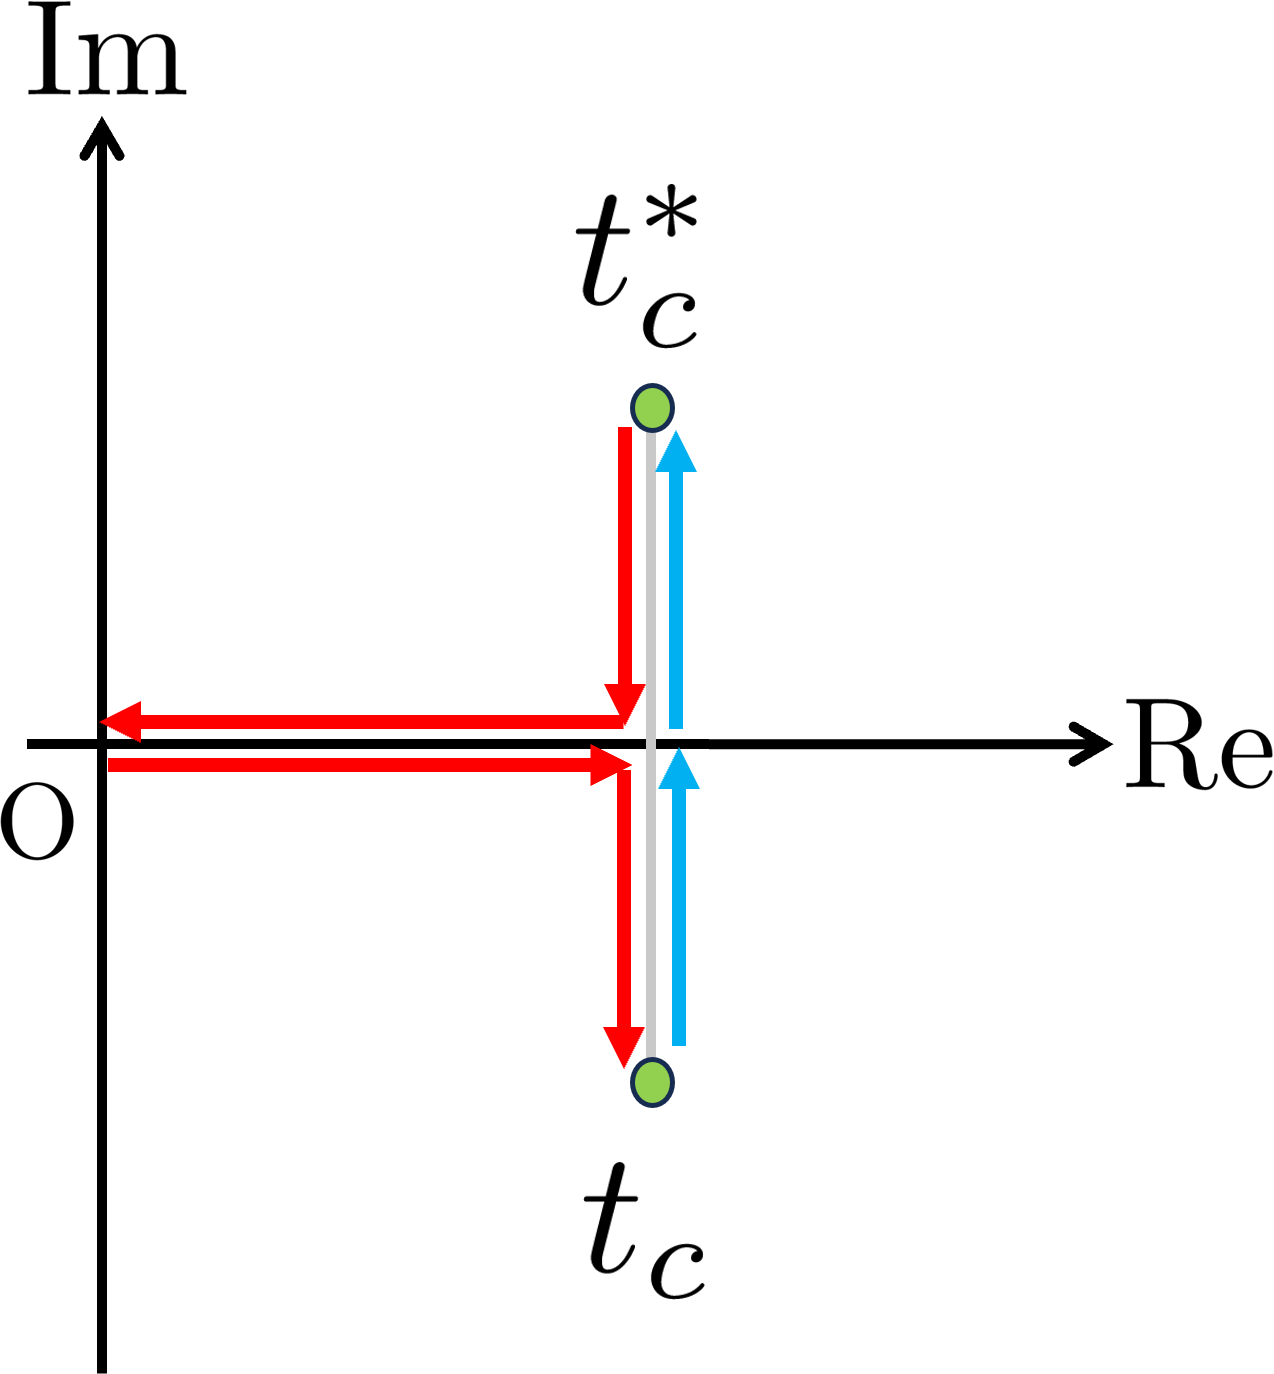
\includegraphics[scale=0.5]{figures/solidangle_GP.png}
  \caption{複素積分(\ref{gamma_g_solid})の経路.赤い線は第1 Riemann面,青い線は第2 Riemann面における経路を表す.また,$t_c$と$t_c^*$を結ぶ緑の線は切断(cut)である.}
  \label{fig:solidangle_GP}
\end{figure}



最後に,$\Gamma_g$の性質を4種類挙げる\cite{Berry1990}.
  \begin{enumerate}
    \item $H(t) = 0$となる$t$が存在するとき,$\Gamma_g = 0$
    \item 時間反転\footnote{$t \rightarrow -t$という変換のこと.}により$\Gamma_g$の符号が変わる
    \item 逆向きの遷移\footnote{今の場合は$|\phi_2(t) \rangle$から$|\phi_1(t) \rangle$への遷移のこと.}で$\Gamma_g$の符号が変わらない
    \item パラメータ空間の軸回りの$\pi$回転にHamiltonianが不変ならば$\Gamma_g = 0$
  \end{enumerate}
特に,性質4は後の議論で重要になる.

\section{Landau-Zener遷移}
Landu-Zener(LZ)遷移\footnote{Majorana,St\"{u}ckelbergの貢献を強調するために,LZMS遷移と呼ぶこともある\cite{Ivakhnenko}.}は,非断熱遷移のもっとも簡単な例である.Landau-Zener遷移が行われる系をLandau-Zener(LZ)モデルと呼ぶ\cite{Zener}.これは,原子の非弾性衝突の確率や磁場における粒子のスピン遷移などの遷移確率を与える重要なモデルである.
LZモデルのHamiltonianは,
\begin{equation}
  \Hat{H}_{\mathrm{LZ}} =
  \begin{pmatrix}
    \varepsilon_0 t & \Delta_0\\
    \Delta_0 & -\varepsilon_0 t
    \label{H_LZ}
  \end{pmatrix}
  \quad (\varepsilon_0 > 0)
\end{equation}
で定義される.ここで,$\varepsilon_0 t$はエネルギーバイアス(energy bias),$\Delta_0$は最小エネルギーギャップ(minimal energy gap)と呼ぶ.また,$\Delta_0 = 0$のときの,Hamiltonian(\ref{H_LZ})についての固有値方程式における固有値を,透熱エネルギー(diabatic energy)と呼ぶ.さらに,それぞれの固有値に属する規格直交化された固有関数を透熱状態(diabatic state)と呼び,属する固有値が小さい順に,$|1\rangle,|2\rangle$で表す\footnote{透熱状態の組を透熱基底と呼ぶ.透熱基底は,断熱基底と同様に完全系をなす.}.


このモデルにおける断熱エネルギーの時間変化を示したのが図\ref{fig:LZ}である.2つの透熱エネルギーが等しくなる部分を準位交差(level crossing)と呼ぶ.また,2つの断熱エネルギーの差がもっとも小さくなる部分では,断熱エネルギーが互いに反発しているように見える.この現象を準位反発(avoided crossing)と呼ぶ.断熱遷移の場合は.初期状態が$| \phi_2(t)\rangle$である系は,準位交差の後も$|\phi_2(t)\rangle$に留まる\footnote{詳しくは第\ref{AT}章を見よ.}.一方,LZ遷移では,準位交差時に状態$|\phi_1(t) \rangle$へ遷移する可能性がある.

\begin{figure}[htbp]
  \centering
  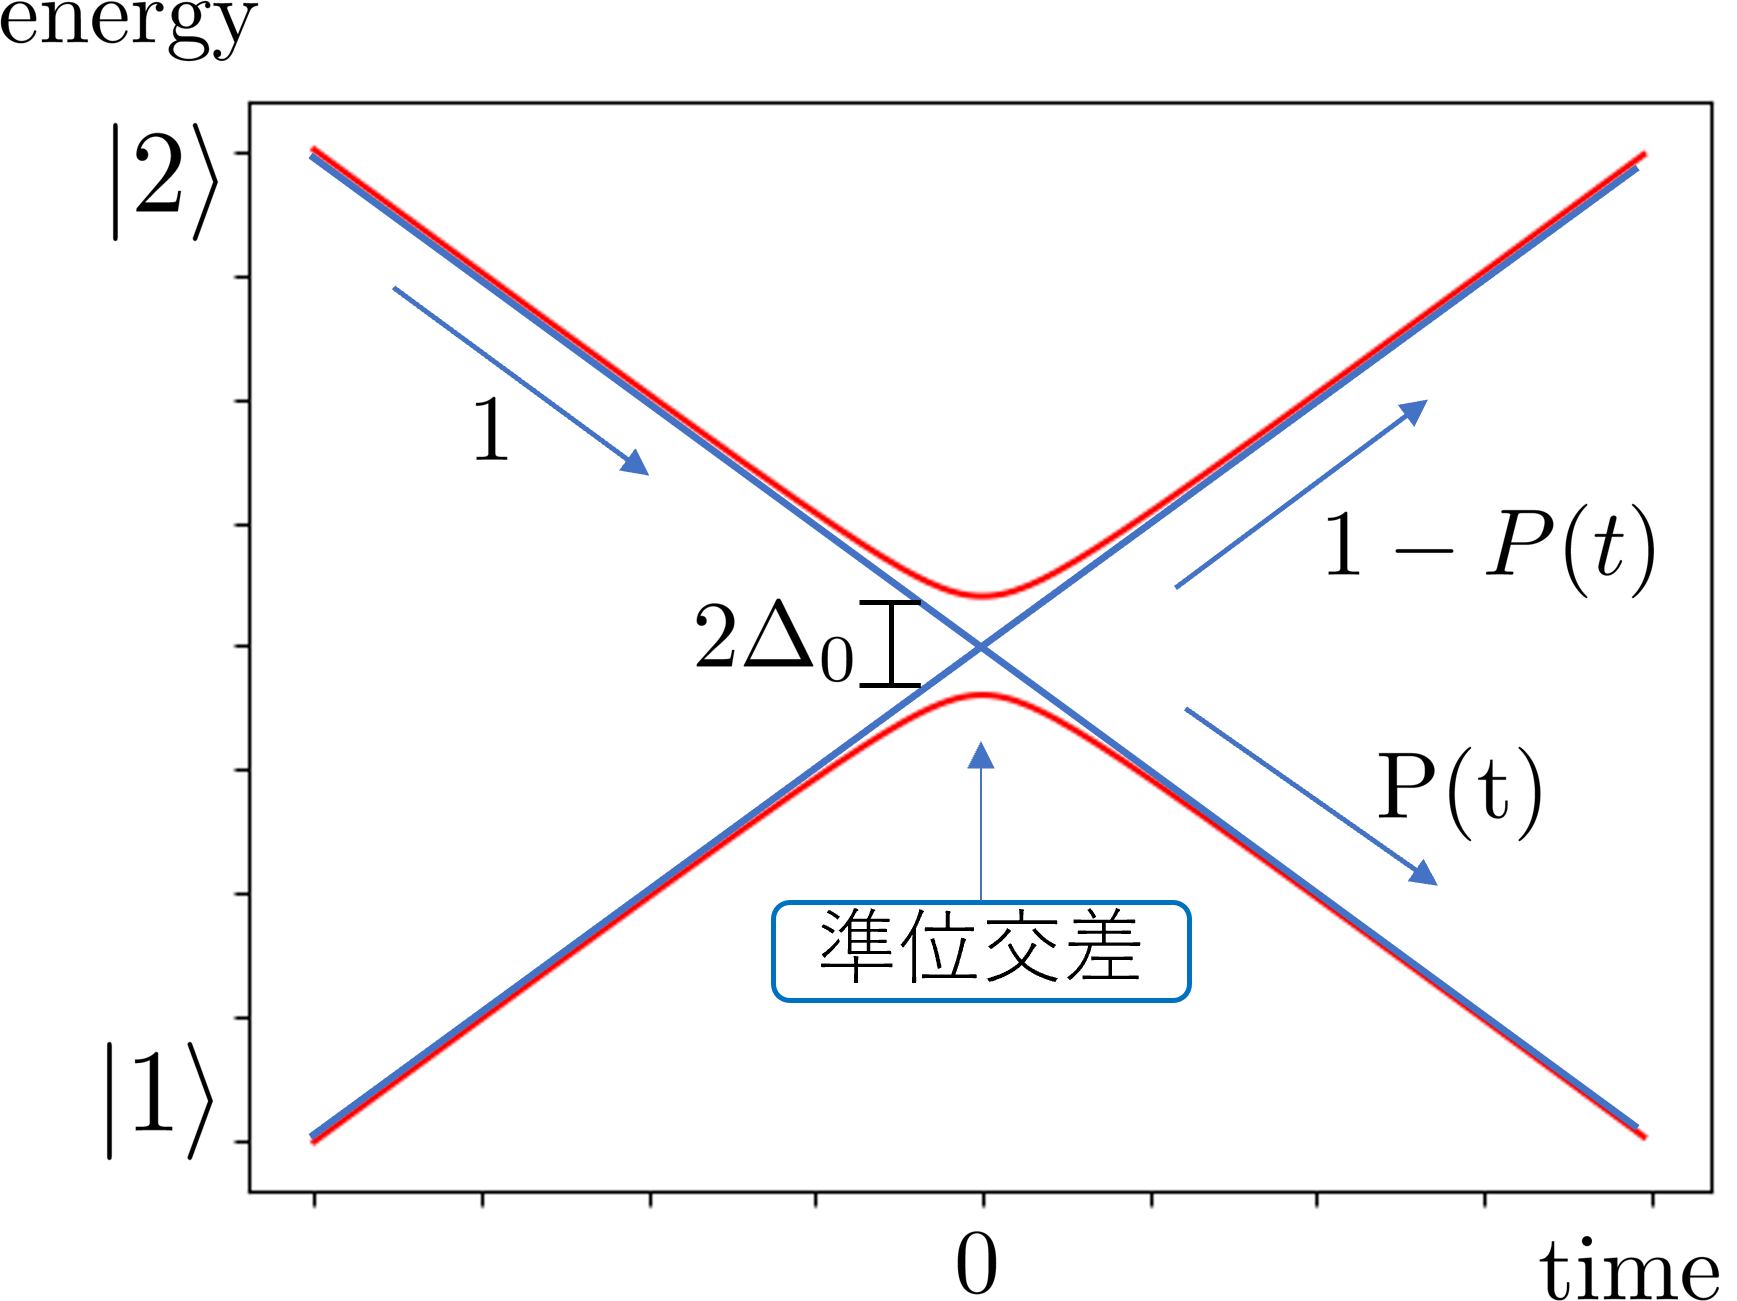
\includegraphics[scale=0.5]{figures/LZ.png}   
  \caption{Landau-Zenerモデルにおける断熱エネルギーの時間変化.赤い線は断熱エネルギー,青い線は透熱エネルギーを示している.$t=0$における断熱エネルギー差は$2\Delta_0$である.}
  \label{fig:LZ}
\end{figure}


この系における$|\phi_2(t)\rangle$から$|\phi_1(t)\rangle$へ遷移する確率$P_{\mathrm{LZ}}$は,
\begin{equation}
  P_{\mathrm{LZ}} = \exp \left(-\frac{\pi \Delta_0^2}{\hbar \varepsilon_0 } \right) 
\end{equation}
であることが知られている.これをLandau-Zener公式と呼ぶ.


また,Pauli行列を基底とするパラメータ空間に,LZモデルのHamiltonian $\Hat{H}_{\mathrm{LZ}}$を描写すると,図\ref{fig:LZ_Pauli}となる.図\ref{fig:LZ_Pauli}および$\Gamma_g$の性質4より,LZモデルでは,幾何学的位相の効果は得られない.

\begin{figure}
  \centering
  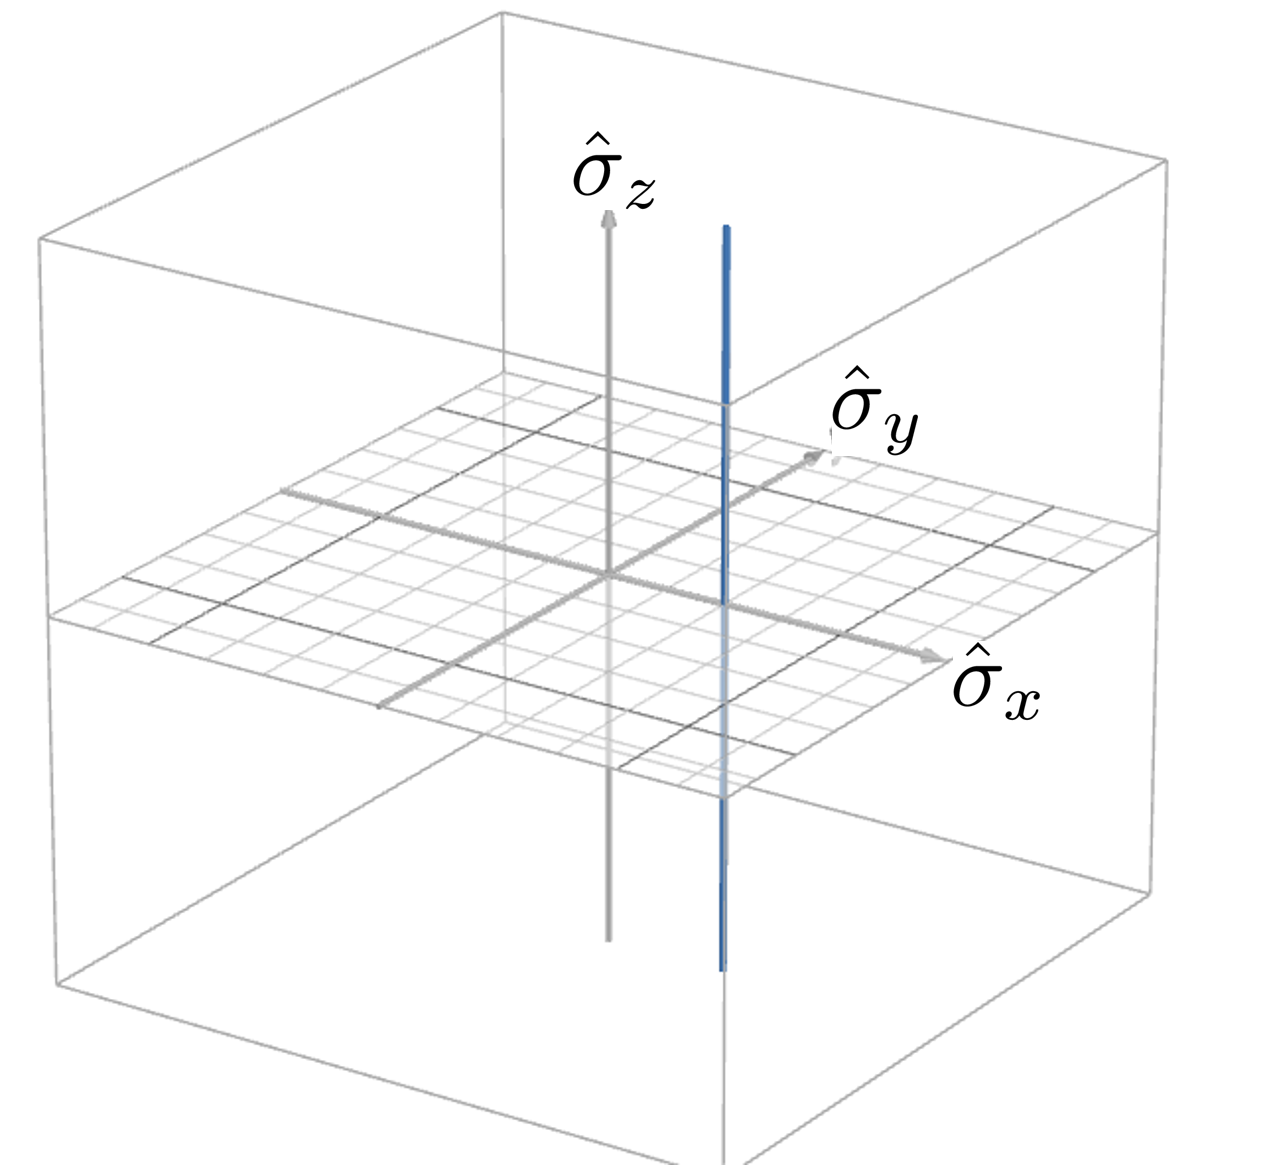
\includegraphics[scale=0.7]{figures/LZ_Pauli.png}
  \caption{Pauli行列を基底とするパラメータ空間におけるLZモデルのHamiltonian $\Hat{H}_{\mathrm{LZ}}$の経路}
  \label{fig:LZ_Pauli}
\end{figure}

\section{Twisted Landau-Zener(TLZ)遷移}
幾何学的位相の効果を具体的に調べるために,BerryはTwisted Landau-Zener(TLZ)モデルを考案した\cite{Berry1990}.TLZモデルのHamiltonianは,
\begin{equation}
 \Hat{H}_{\mathrm{TLZ}} =\Delta_0 \cos \phi(t) \Hat{\sigma}_x + \Delta_y \sin \phi(t) \Hat{\sigma}_y + \varepsilon_0 t \Hat{\sigma}_z
\end{equation}
である\footnote{Berryが提唱したTLZモデルは,厳密には$\Delta_0 = \Delta_y$の場合に限定される.ここでは,$x$成分と$y$成分のパラメータをそれぞれ自由に決められるようにしている.}.ただし,$\Delta_y$は任意の定数,$\phi(t)$は任意の$t$の関数,$t = \delta \tau$である.


LZモデルと同様に,Pauli行列を基底としたパラメータ空間に$H_{\mathrm{TLZ}}$を描写すると,図\ref{fig:uniform_helix}および図\ref{fig:winding_helix}のようになる.これらの図および$\Gamma_g$の性質4より,$\phi(t) \propto t$のように$\phi(t)$が奇関数のときは幾何学的位相の効果は得られない.一方,$\phi(t) \propto t^2$のように$\phi(t)$が偶関数のときは幾何学的位相の効果を得られる.

\begin{figure}[htbp]
  \centering
  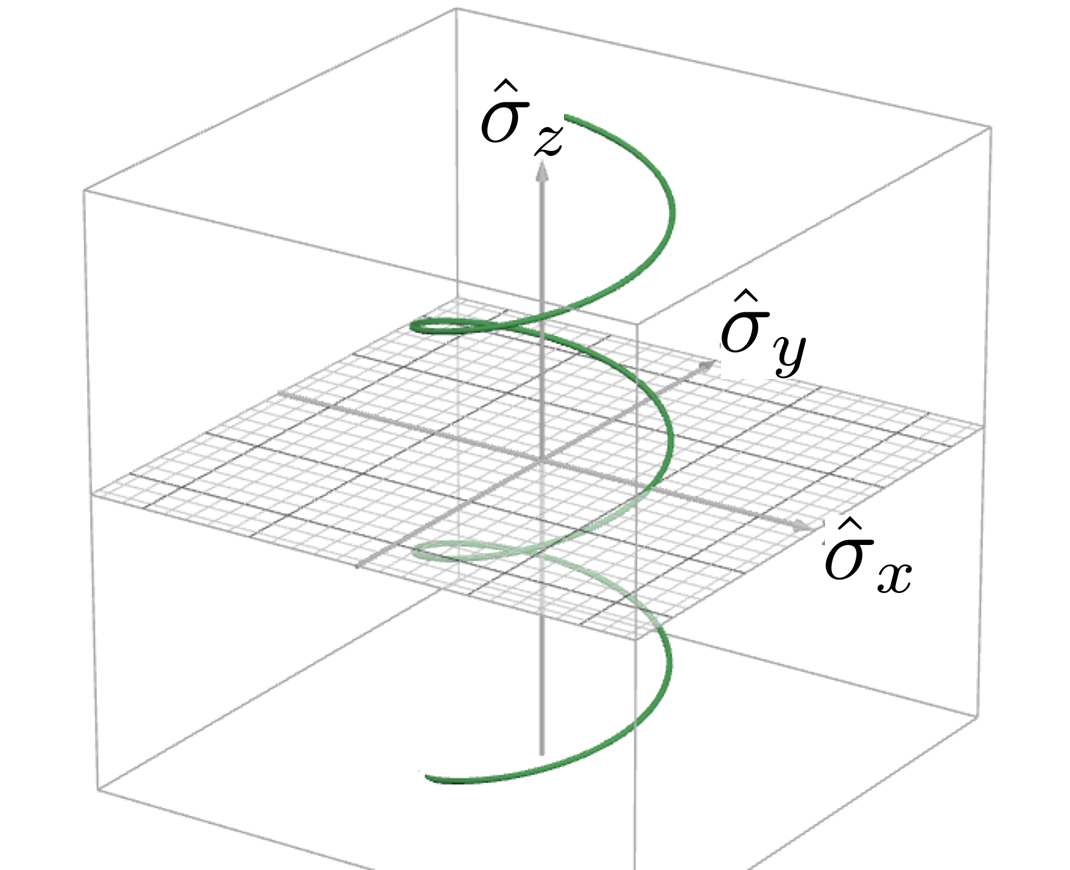
\includegraphics[scale=0.8]{figures/uniform_helix.png}
  \caption{$\phi(t) \propto t$における$H_{\mathrm{TLZ}}$の経路.この図形をuniform helixと呼ぶ.}
  \label{fig:uniform_helix}
\end{figure}

\begin{figure}[htbp]
  \centering
  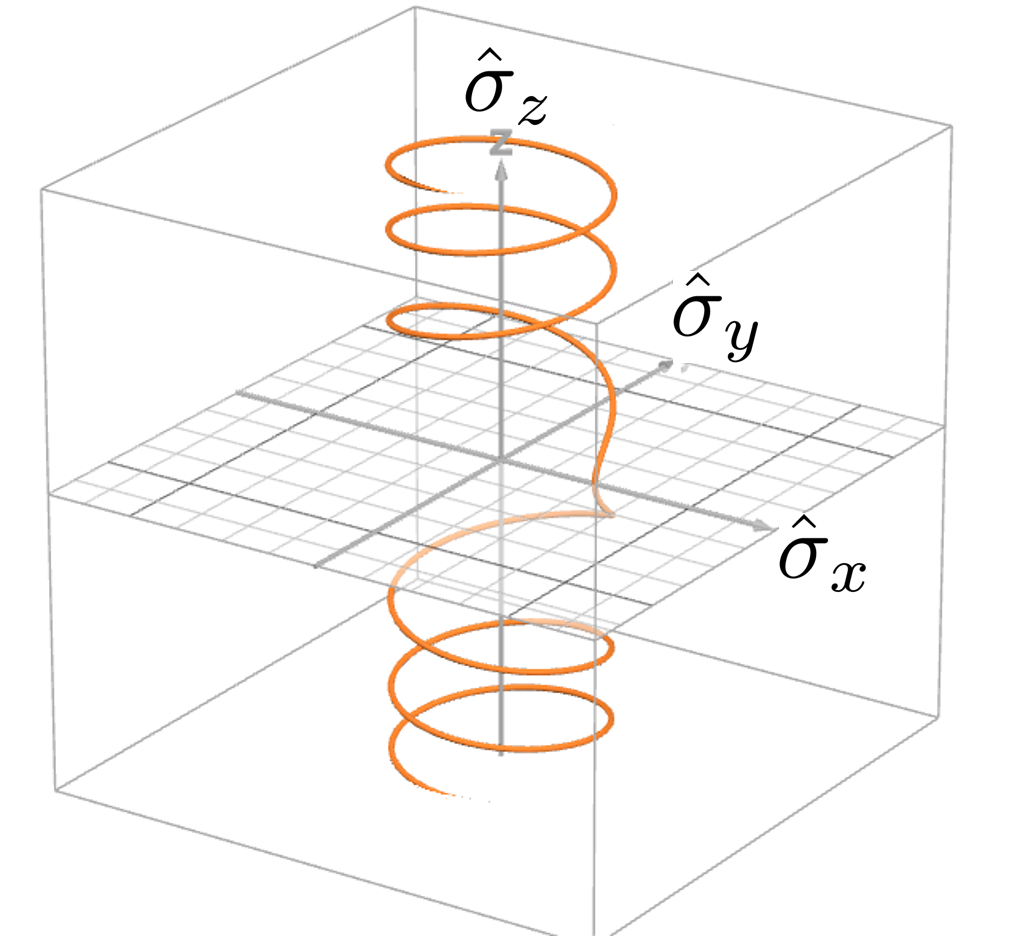
\includegraphics[scale=0.8]{figures/winding_helix.png}
  \caption{$\phi(t) \propto t^2$における$H_{\mathrm{TLZ}}$の経路.この図形をwinding-unwinding helixと呼ぶ.}
  \label{fig:winding_helix}
\end{figure}

$\phi(t) \propto t^2$の場合について,詳しく見てみよう.$\Delta_y = \frac{1}{2} \kappa_g \varepsilon_0^2$として$t^2$の項まで展開すると,
\begin{equation}
  \Hat{H}_{\mathrm{TLZ}} = \Delta_0 \, \Hat{\sigma}_x + \frac{1}{2} \kappa_g \varepsilon_0^2 (\delta \tau)^2 \, \Hat{\sigma}_y + \varepsilon_0 \delta \tau \, \Hat{\sigma}_z
\end{equation}
となる.ただし,$\kappa_g$は${\tau}=0$における測地曲率である.


ここで,測地曲率について説明しよう.ある曲面$S$を通る曲線$C(s)$があるとする.この曲線$C(s)$の1階微分および2階微分
\begin{equation}
  \frac{d C(s)}{d s}, \frac{d^2 C(s)}{d s^2}
\end{equation}
をそれぞれ曲線の接ベクトル,曲率ベクトルと呼ぶ.また,曲面$S$の法ベクトルを$\bm{n}(s)$とする.このとき,
\begin{equation}
  \kappa_g =  \left(\bm{n}(s) \times \frac{d C(s)}{d s} \right)\cdot \frac{d^2 C(s)}{d s^2}
\end{equation}
を測地曲率と呼ぶ.TLZモデルにおける測地曲率のイメージ図を図\ref{fig:geodesic_curvature}で示しておく.青い矢印で表される曲率ベクトルを灰色の接平面に射影したときの長さが測地曲率である.


\begin{figure}[hpbt]
  \centering
  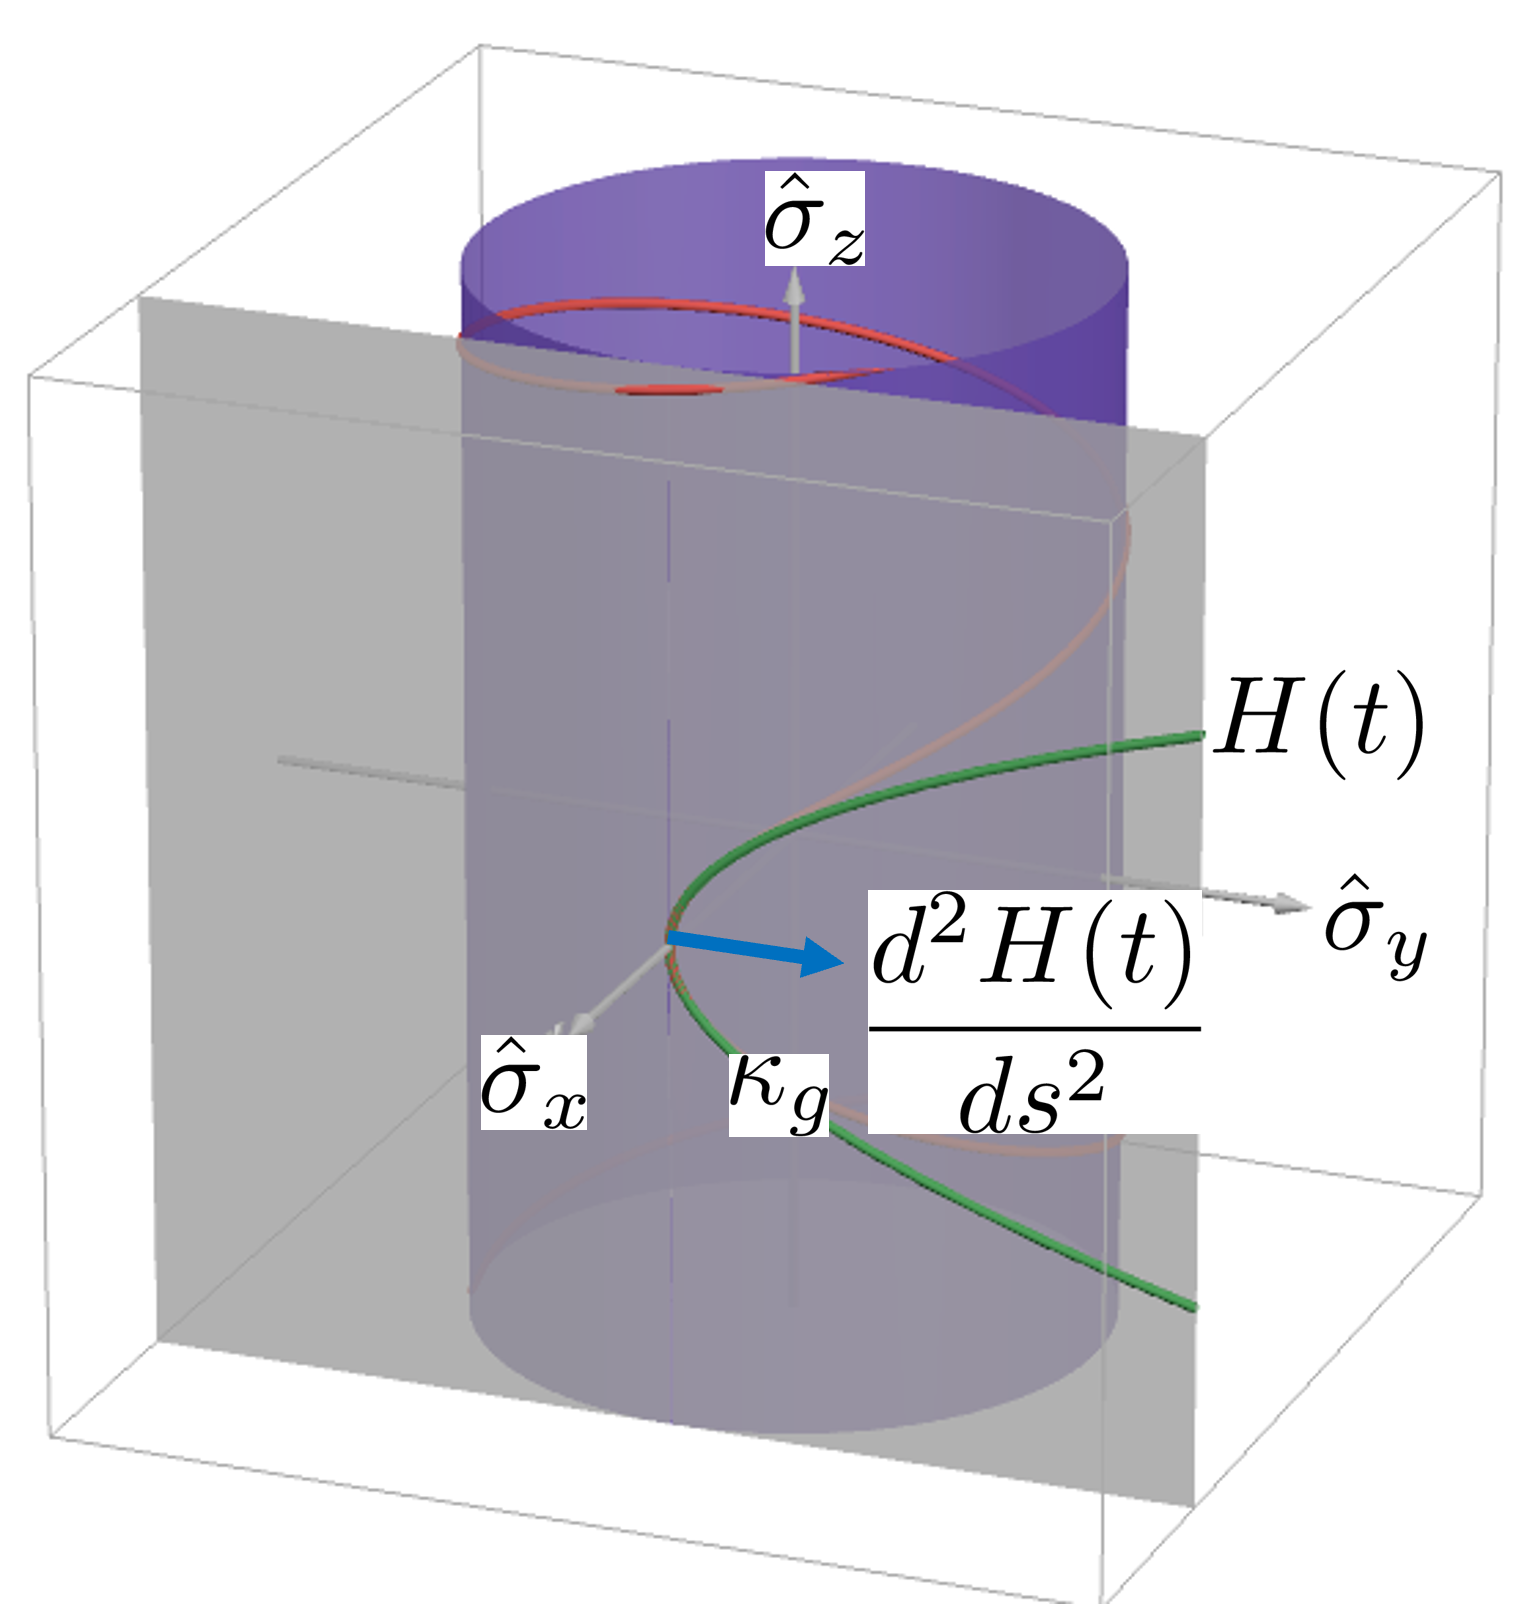
\includegraphics[scale=0.7]{figures/geodesic_curvature.png}
  \caption{TLZモデルにおける測地曲率のイメージ図.オレンジ線がTLZモデルの経路である.緑線はTLZモデルを2次展開したときの経路である.青矢印は,TLZモデルにおける曲率ベクトルである.紫色の面はTLZモデルの経路が通る曲面である.灰色の面は${\tau}=0$における紫色の面の接平面である.}
  \label{fig:geodesic_curvature}
\end{figure}


このモデルにおける遷移確率は,
\begin{equation}
  P(\delta) = \exp \left[-\pi \frac{(\Delta_0 -\frac{\kappa_g \varepsilon_0 \delta}{4})^2}{\varepsilon_0 |\delta|}\right] \label{TLZ_TP}
\end{equation}
となることが知られている\cite{Oka}.次節でこの遷移確率を導出する.また,QGPを用いて書き換えると,
\begin{equation}
  P(\delta) = \exp \left[-\frac{\pi}{4\varepsilon_0 |\delta|} \left(\Delta_0 + \frac{\delta \Delta_{21}}{2}\right)\right]
\end{equation}
となる.この式は,Landau-Zenerモデルにおいて,
\begin{equation}
  \Delta_0 \rightarrow \Delta_0 + \frac{\delta \Delta_{21}}{2}
\end{equation}
と置き換えた形になっている.そのため,幾何学的効果は,エネルギーギャップをシフトさせることを明示的に教えてくれる.$P(\delta)$のグラフは図\ref{fig:Curvature_Effect}のようになる.LZモデルの場合は,$P(\delta)$のグラフは$\delta$の符号に対称である.一方,TLZモデルの場合は,$P(\delta)$のグラフが$\delta$の符号に非対称になる.この非対称性を,整流作用(rectification)と呼ぶ.特に,$P(\delta)=1$となる$\delta$が存在することが重要である.この現象を完全トンネル(perfect tunneling)という.

\begin{figure}
  \centering
  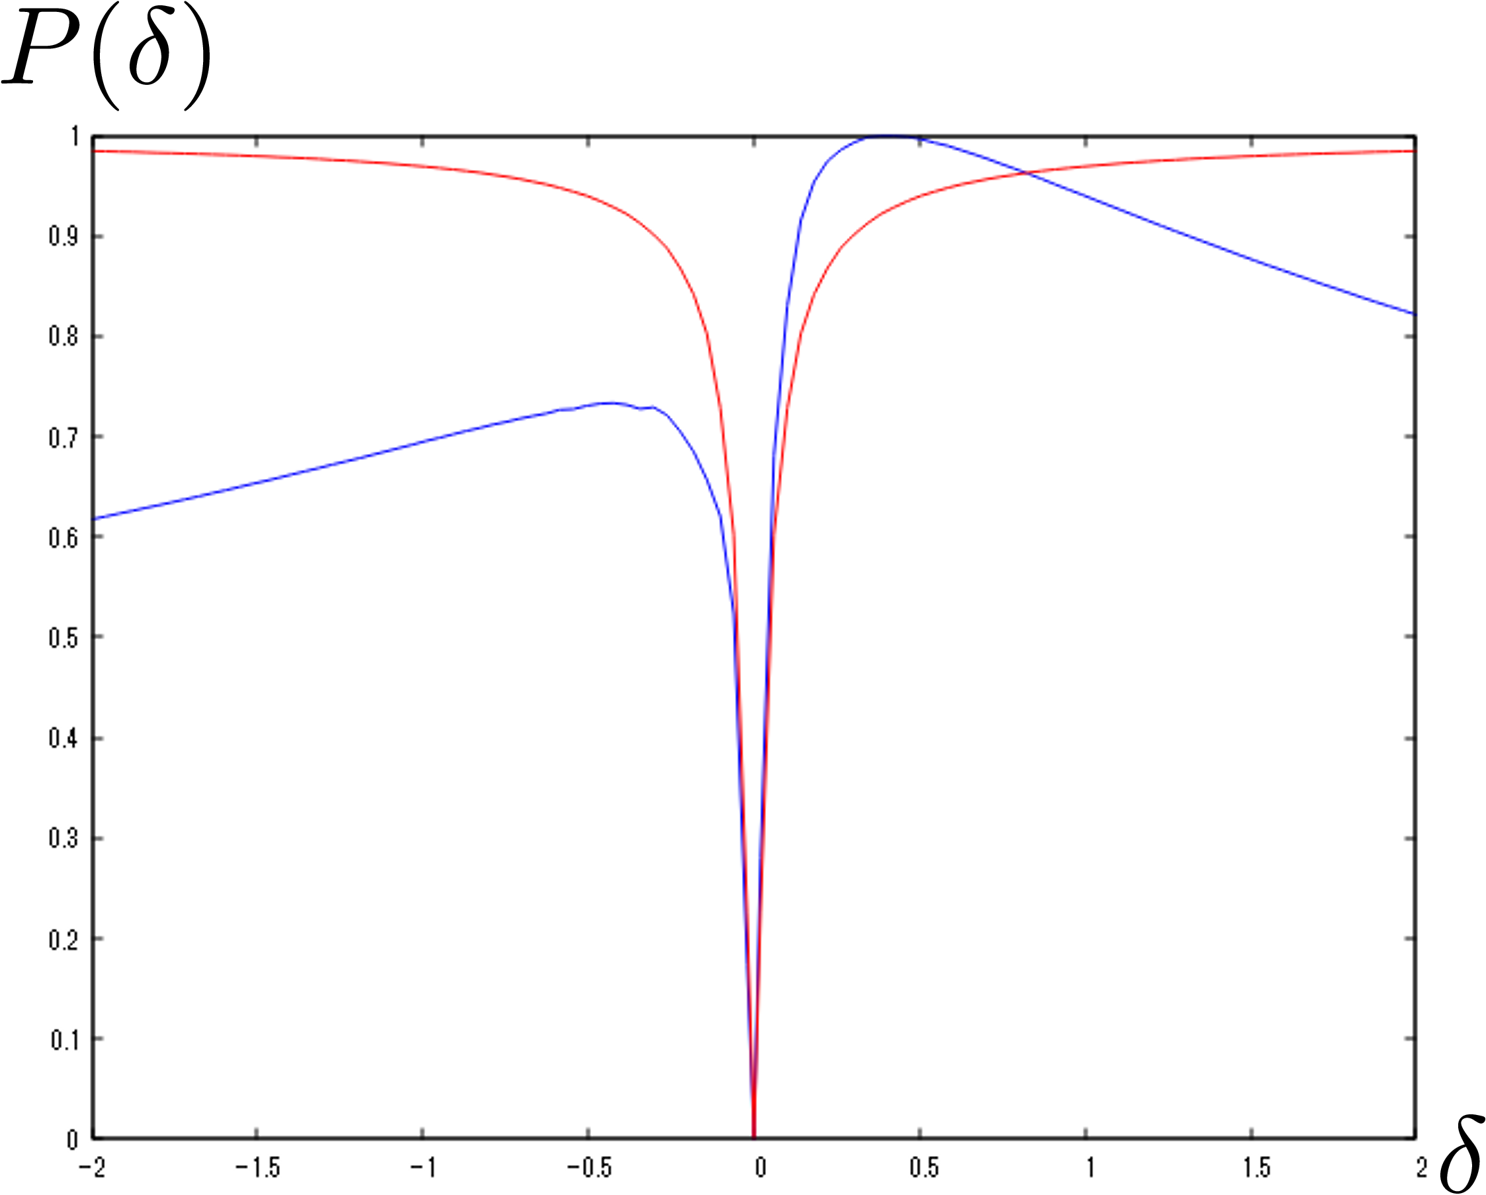
\includegraphics[scale=0.7]{figures/Curvature_Effect.png}
  \caption{$P(\delta)$の$\delta$依存性を示したグラフ.$\varepsilon_0 = 1, \Delta_0 =0.1$である.また,青い線は$\kappa_g = 1$,赤い線は$\kappa_g = 0$の場合を表す.}
  \label{fig:Curvature_Effect}
\end{figure}

\section{TLZモデルにおける遷移確率の導出}
本節では,式(\ref{TLZ_TP})を導出する.そのために,
\begin{equation}
  \bm{d}(t) := (x(t),y(t),z(t))^T \label{d}
\end{equation}
として,$t=0$における3つの量
\begin{align}
  \bm{r} &:= \frac{\bm{d}(0)}{|\bm{d}(0)|} \label{r}\\
  \bm{t} &:= \frac{\partial_{\tau} \bm{d}(0)}{|\partial_{\tau} \bm{d}(0)|} \label{t}\\
  \bm{n} &:= \bm{r}\times \bm{t} \label{n}
\end{align}
を定義する.$\bm{r}$,$\bm{t}$,$\bm{n}$はそれぞれ動径ベクトル,接ベクトル,法ベクトルである.今の系では,式(\ref{d})が,
\begin{equation}
  \bm{d} =
  \begin{pmatrix}
    \Delta_0\\
    \frac{1}{2} \kappa_g \varepsilon_0^2 t^2\\
    \varepsilon_0 t\\
  \end{pmatrix}
\end{equation}
である場合を考えればよい.このとき,動径ベクトル(\ref{r}),接ベクトル(\ref{t}),法ベクトル(\ref{n})はそれぞれ,
\begin{equation}
  \bm{r} =
  \begin{pmatrix}
    1\\
    0\\
    0\\
  \end{pmatrix}, \quad
  \bm{t} =
  \begin{pmatrix}
    0\\
    0\\
    1\\
  \end{pmatrix}, \quad
  \bm{n} =
  \begin{pmatrix}
    0\\
    1\\
    0\\
  \end{pmatrix}
\end{equation}
となる.ここで,
\begin{align}
  a(t) &:= \bm{d}(t)\cdot \bm{t} = z\\
  b(t) &:= \sqrt{|\bm{d}(t)|^2-a(t)^2} = \sqrt{x^2+y^2}
\end{align}
を定義すると,
\begin{equation}
  \Hat{U}^{\dagger} \Hat{H} \Hat{U}
  = \left( a(t)\bm{t} + b(t) \bm{r} \right) \cdot \Hat{\bm{\sigma}}
\end{equation}
と表せる.したがって,
\begin{align}
  a(t)
  &= 
  \begin{pmatrix}
    \Delta_0\\
    \frac{1}{2} \kappa_g \varepsilon_0^2 t^2\\
    \varepsilon_0 t\\
  \end{pmatrix}
  \cdot
  \begin{pmatrix}
    1\\
    0\\
    0\\
  \end{pmatrix}\\
  &=
  \Delta_0,\\
  b(t)
  &=
  \sqrt{\left|
  \begin{pmatrix}
    \Delta_0\\
    \frac{1}{2} \kappa_g \varepsilon_0^2 t^2\\
    \varepsilon_0 t\\
  \end{pmatrix}
  \right|^2 -\Delta_0^2}\\
  &= \sqrt{(\varepsilon_0 t)^2 + (\frac{1}{2} \kappa_g \varepsilon_0^2 t^2)^2}\\
  &\approx \varepsilon_0 t (1+ (\frac{1}{2} \kappa_g \varepsilon_0 \tau)^2)^{\frac{1}{2}}\\
  &= \varepsilon_0 t + O(t^3),\\
  \phi(t)
  &= \arctan \frac{\kappa_g \varepsilon_0 t}{2} \label{phi_arc}
\end{align}
である.また,式(\ref{phi_arc})の両辺を$t$で微分すると,
\begin{align}
  \partial_t \phi(t)
  &= \frac{\frac{\kappa_g \varepsilon_0 t}{2}}{1+(\frac{\kappa_g \varepsilon_0 t}{2})^2}\\
  &= \frac{\kappa_g \varepsilon_0}{2} (1-(\frac{\kappa_g \varepsilon_0 t}{2})^2)^{-1}\\
  &= \frac{\kappa_g \varepsilon_0}{2} + O(t^2)
\end{align}
となる.さらに,断熱エネルギー(\ref{E_LZ})は,
\begin{equation}
  E_{\mathrm{LZ}_2}(t) \approx  \sqrt{\left(\Delta_0 - \left(\frac{\kappa_g \varepsilon_0 \delta }{4}\right) \right)^2 + (\varepsilon_0 t)^2}
\end{equation}
である.$E_{\mathrm{LZ}_2}(t_c) = 0$となる,断熱エネルギー$E_{\mathrm{LZ}_2}(t_c)$の零点$t_c$は,
\begin{equation}
  t_c = \frac{i}{\varepsilon_0} \left( \Delta_0 - \left(\frac{\kappa_g \varepsilon_0 \delta}{4}\right) \right)
\end{equation}
と定まる.よって,TLZ遷移における遷移確率(\ref{P_nt})は,
\begin{align}
  P
  &\approx \exp \left(\frac{4}{|\delta|} \mathrm{Im} \int_0^{t_c} \sqrt{\left( \left( \Delta_0 - \left(\frac{\kappa_g \varepsilon_0 \delta }{4}\right) \right)^2 + (\varepsilon_0 t)^2 \right)} dt \right)\\
  &= \exp \left(\frac{4}{|\delta|} \int_0^{\frac{1}{\varepsilon_0} (\Delta_0 - \frac{\kappa_g \varepsilon_0 \delta}{4})} \sqrt{\left( \left( \Delta_0 - \left(\frac{\kappa_g \varepsilon_0 \delta}{4} \right)\right)^2 - (\varepsilon_0 t)^2 \right)} dt \right)
\end{align}
である.ここで,積分を実行するために,変数変換
\begin{equation}
  t = \frac{1}{\varepsilon_0} \left(\Delta_0 - \frac{\kappa_g \varepsilon_0 \delta}{4} \right) \cos \varphi
\end{equation}
を行うと,
\begin{align}
  P
  &= \exp \left(\frac{4}{|\delta|} \int_{\frac{\pi}{2}}^0 \sqrt{\left(\Delta_0 - \left(\frac{\kappa_g \varepsilon_0 \delta}{4}\right) \right)^2 (1-\cos^2\varphi)} \frac{1}{\varepsilon_0} \left( \Delta_0 - \frac{\kappa_g \varepsilon_0 \delta}{4} \right) (-\sin \varphi) d\varphi \right)\\
  &= \exp \left(-\frac{4}{\varepsilon_0 |\delta|} \left(\Delta_0 - \frac{\kappa_g \varepsilon_0 \delta}{4} \right) ^2\int_0^{\frac{\pi}{2}} \sin^2\theta d\theta \right)\\
  &= \exp \left(-\frac{4}{\varepsilon_0 |\delta|} \left(\Delta_0 - \frac{\kappa_g \varepsilon_0 \delta}{4} \right) ^2 \frac{\pi}{4} \right)\\
  &= \exp \left(-\frac{\pi}{4} \frac{(2\Delta_0-\frac{\kappa_g \varepsilon_0 \delta}{4})^2}{\varepsilon_0 |\delta|} \right)\\
  &= \exp \left[-\pi \frac{(\Delta_0 -\frac{\kappa_g \varepsilon_0 \delta}{4})^2}{\varepsilon_0 |\delta|}\right]
\end{align}
となり,式(\ref{TLZ_TP})が示された.


\chapter{cyclic evolution}\label{CE}
本章では,cyclic evolutionを説明する.特に,LZ遷移を含むcyclic evolutionは,その代表例である.


\section{序論}
本論文では,cyclic evolutionとは,時間発展の後,Hamiltonianが初期状態に戻るような系のことを指すものとする\footnote{多くの場合,cyclic evolutionは,状態ベクトルが初期状態に戻るような時間発展を指す.}.このようなHamiltonianは,Pauli行列を基底としたパラメータ空間内で閉曲線を描く.


第\ref{AT}章で,Berry位相を定義した.この位相を,断熱条件が成り立たない場合に拡張したものをAharonov-Anandan位相と呼ぶ.系の状態ベクトルが初期状態に戻るような系でAharonov-Anandan位相が定義できる\cite{Aharonov}.



\section{LZ遷移を含むcyclic evolution}
cyclic evolutionの例として,LZ遷移を周期的に繰り返す系を考えよう\cite{Kayanuma1993}.この系のHamiltonianは,
\begin{align}
  \Hat{H}_{\mathrm{CE}}
  &=
  \begin{pmatrix}
    \varepsilon_0 \cos \omega t& \Delta_0 C(t)\\
    \Delta_0 C(t) & -\varepsilon_0 \cos \omega t
  \end{pmatrix} \\
  &= \Delta_0 C(t) \, \Hat{\sigma}_x + \varepsilon_0 \cos \omega t \, \Hat{\sigma}_z \label{H_CE_LZ}
\end{align}
で表される.ただし,$\omega$は角振動数である.


この系における断熱エネルギーの時間変化は図\ref{fig:CE_LZ}のようになる.図\ref{fig:CE_LZ}から,断熱エネルギーは周期的に準位交差することがわかる.また,パウリ行列を基底とするパラメータ空間にHamiltonianを描写すると図\ref{fig:CE_LZ_Pauli}のようになる.図\ref{fig:CE_LZ_Pauli}より,Hamiltonianが閉曲線を描いているため,この系はcyclic evolutionである.

\begin{figure}[htbp]
  \centering
  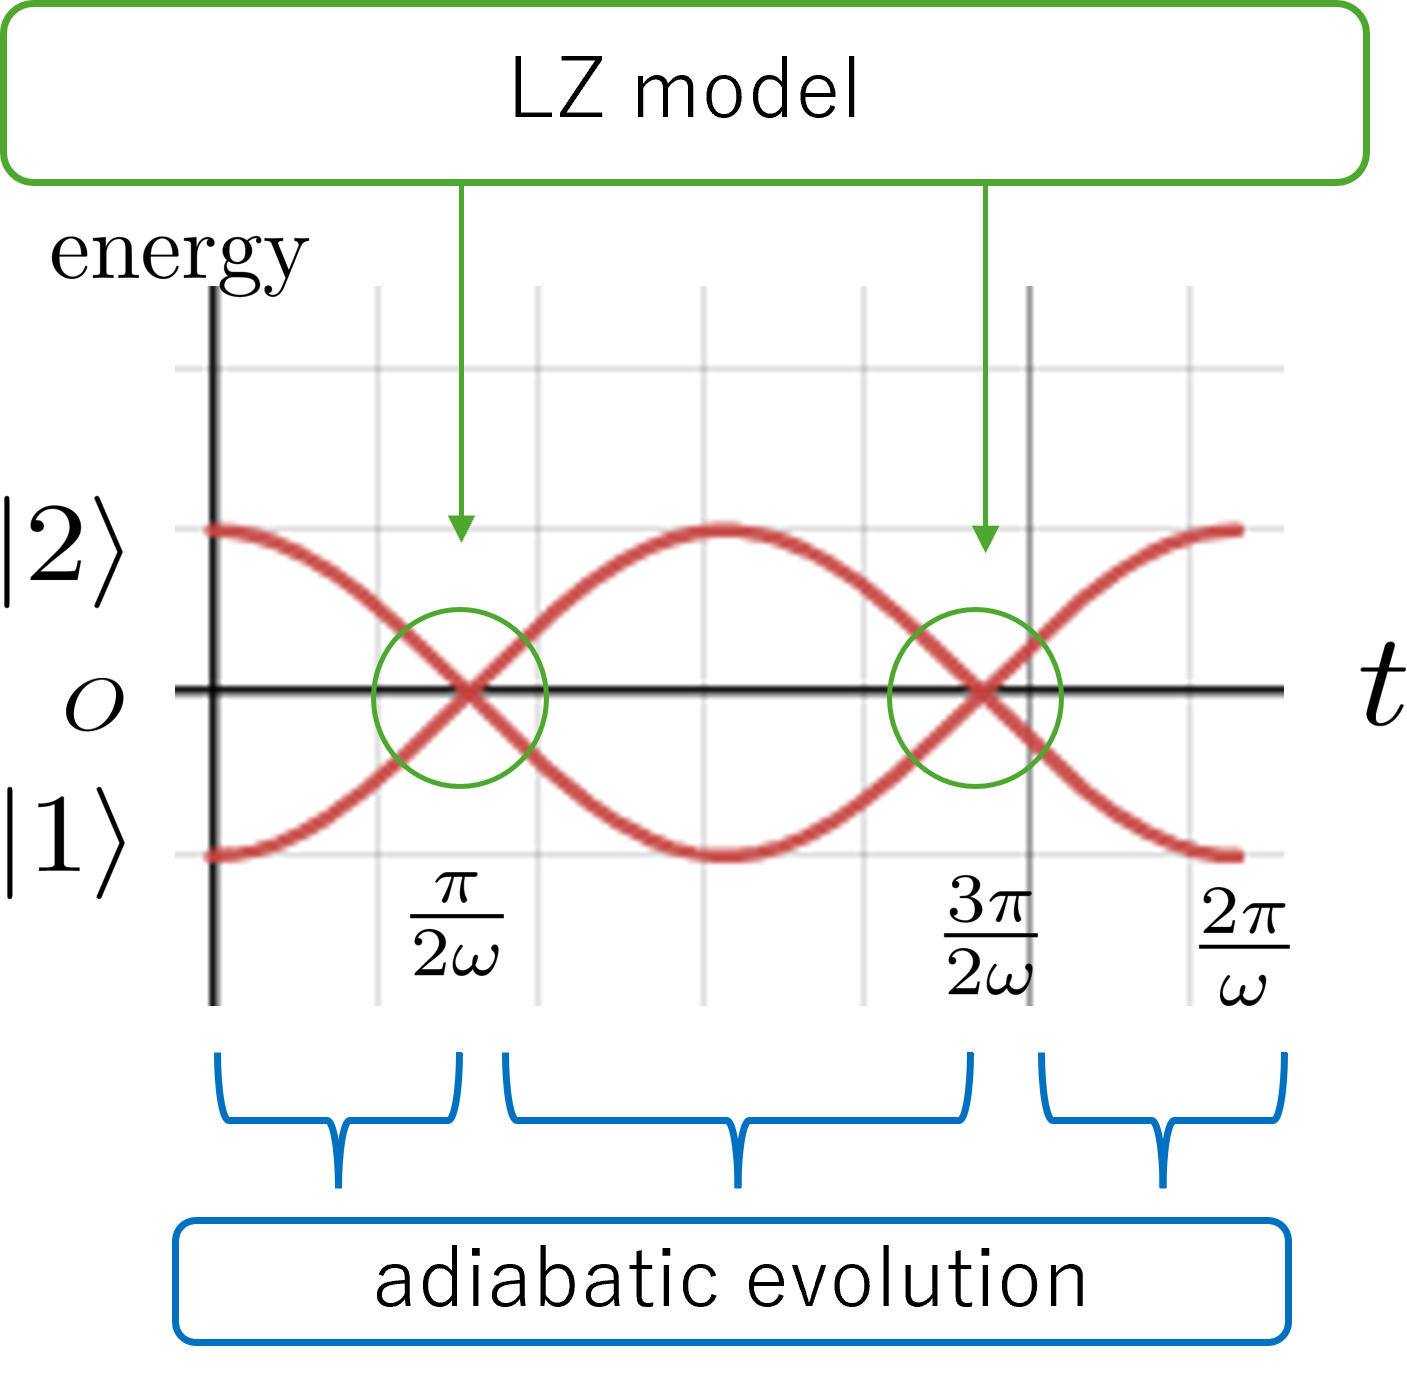
\includegraphics[scale=0.7]{figures/CE_LZ.png}
  \caption{LZ遷移を含むcyclic evolutionにおける断熱エネルギーの時間変化}
  \label{fig:CE_LZ}
\end{figure}

\begin{figure}[htbp]
  \centering
  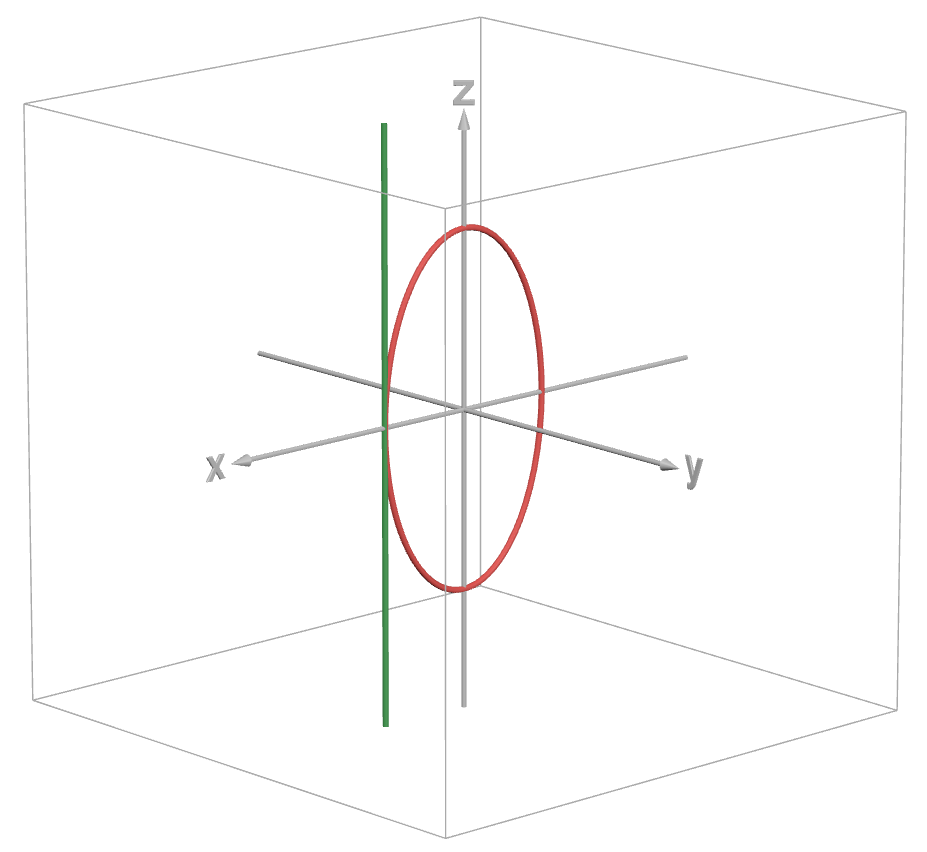
\includegraphics[scale=0.3]{figures/CE_LZ_Pauli.png}
  \caption{LZ遷移を含むcyclic evolutionにおけるHamiltonanの経路を赤い線で示している.緑の線は1回のLZ遷移である.}
  \label{fig:CE_LZ_Pauli}
\end{figure}


この系における,各準位交差後の波動関数を求めよう.ここで,$\Delta_0 \ll \varepsilon_0 $のとき,転送行列法を用いることができる.転送行列法では,この系を3つの部分
\begin{enumerate}
  \item 断熱エネルギー差がもっとも大きくなる時点から準位交差直前までの断熱的な時間発展
  \item 準位交差付近のLZ遷移
  \item 準位交差直後から,断熱エネルギー差がもっとも大きくなる時点までの断熱的な時間発展
\end{enumerate}
に分割する.また,$2 \times 2$行列
\begin{align}
  M &= 
  \begin{pmatrix}
    \sqrt{q} & -\sqrt{1-q} e^{i\phi_s}\\
    \sqrt{1-q} e^{i\phi_s} & \sqrt{q}
  \end{pmatrix},\\
  H &=
  \begin{pmatrix}
    e^{i\eta}  & 0\\
    0 & e^{-i\eta}
  \end{pmatrix},\\
  G &= 
  \begin{pmatrix}
    e^{i\theta}  & 0\\
    0 & e^{-i\theta}
  \end{pmatrix}
\end{align}
を定義する.ただし,
\begin{align}
  q &:= \exp(-2\pi \bar{\delta}),\\
  \bar{\delta} &:= \frac{\Delta_0^2}{2\varepsilon_0 \omega},\\
  \eta (t) &:= \int_0^t dt^{\prime} \sqrt{(\varepsilon_0 \cos\omega t)^2+ (\Delta_0 C(t))^2},\\
  \theta &:= 2 \int_0^{\frac{\pi}{2\omega}} dt \sqrt{(\varepsilon_0 \cos\omega t)^2+ (\Delta_0 C(t))^2} = 2 \eta(\frac{\pi}{2\omega}),\\
  \phi_s &:= \frac{\pi}{4} + \arg \Gamma(1-i\bar{\delta}) + \bar{\delta}(\ln \bar{\delta} -1)
\end{align}
である\footnote{特に,$\phi_s$は,Stokes位相と呼ばれ,Landau-Zener遷移前後における位相の変化を議論する際に重要である.}.さらに,ある行列$A$と一対一に対応する行列を$A^{\prime}$で表す\footnote{$C(t)$の具体形によって,対応する行列が変わるため,曖昧に記述している.$A^{\prime}$は,$A$の複素共役行列や転置行列である場合が多い.}.例えば,$C(t) = 1$,$C(t) = \sin \omega t$のとき,$A^{\prime}$はそれぞれ$A$の転置行列,複素共役行列になる.このとき,$t=0$における波動関数を$\psi_0 = (1,0)^T$とすると,$t = \frac{\pi}{\omega}, \frac{2\pi}{\omega}, \ldots, \frac{(2m-1)\pi}{\omega}, \frac{2m \pi}{\omega} , \ldots$における波動関数$\psi_1, \psi_2, \ldots,\psi_{2m-1} , \psi_{2m}, \ldots$は,
\begin{align}
  \psi_1 &= G^{\frac{1}{2}} M G^{\prime \frac{1}{2}} \psi_0,\\
  \psi_2 &=  G^{\prime \frac{1}{2}} M^* G M G^{\prime \frac{1}{2}} \psi(0),\\
  \vdots \notag \\
  \psi_{(2m-1)} &= (G^{\frac{1}{2}} M G^{\prime \frac{1}{2}}) (G^{\prime \frac{1}{2}} M^{\prime} G M G^{\prime \frac{1}{2}})^{m-1} \psi_0,\\
  \psi_{2m} &= (G^{\prime \frac{1}{2}} M^{\prime} G M G^{\prime \frac{1}{2}})^{m} \psi_0,\\
  \vdots \notag
\end{align}
で表される.

\section{転送行列$M$の決定}
本節では,転送行列$M$が,
\begin{equation}
  M =
  \begin{pmatrix}
    e^{-\pi\bar{\delta}} & -\sqrt{1-e^{-2\pi\bar{\delta}}} e^{i\phi_s}\\
    \sqrt{1-e^{-2\pi\bar{\delta}}} e^{-i\phi_s} & e^{-\pi\bar{\delta}} 
  \end{pmatrix}
\end{equation}
となることを示す\footnote{付録Aも参照せよ.}.


そのために,準位交差直前の状態$(c_1^-, c_2^-)$から準位交差後の状態$(c_1^-, c_2^-)$が導かれることを仮定する.すなわち,ある行列$M$を用いて,
\begin{equation}
  \begin{pmatrix}
    c_1^+\\
    c_2^+
  \end{pmatrix}
  =
  \begin{pmatrix}
    M_{11} & M_{12}\\
    M_{21} & M_{22}
  \end{pmatrix}
  \begin{pmatrix}
    c_1^-\\
    c_2^-
  \end{pmatrix}
\end{equation}
と書けるものとする.また,議論の見通しを良くするため,$\varepsilon_0 \rightarrow -v/2$とする.

まず,$M_{11}$を求める.Shr\"{o}dinger方程式(\ref{SE})に,系のHamiltonian(\ref{H_CE_LZ})を代入して,
\begin{equation}
  i\frac{d}{dt} c_1(t) = -\frac{vt}{2} c_1(t) + \Delta_0 c_2(t)
\end{equation}
となる.ここで,
\begin{align}
  z &= i\sqrt{v} e^{i\frac{\pi}{4}} t\\
  n &= i\bar{\delta}\\
  \bar{\delta} &= \frac{\Delta_0^2}{v} \label{delta_bar}\\
  c_1 &= w_1(z)\\
  c_2 &= w_2(z)
\end{align}
という変数変換を行って整理すると,
\begin{equation}
  \left( \frac{d}{dz} + \frac{z}{2} \right) w_1 = - e^{-\frac{i\pi}{4}} \frac{\Delta_0}{\sqrt{v}} w_2 \label{M11}
\end{equation}
となる.ここで,定理
\begin{equation}
  \left( \frac{d}{dz} + \frac{z}{2} \right) D_n(z) = n D_{n-1} (z)
\end{equation}
を用いると,
\begin{align}
  \text{(\ref{M11})の左辺} &= A \left( \frac{d}{dz} + \frac{z}{2}\right) D_n(z) = A n D_{n-1}(z)\\
  \text{(\ref{M11})の右辺} &= - e^{-\frac{i\pi}{4}} \frac{\Delta_0}{\sqrt{v}} B D_{n-1}(z)
\end{align}
である.したがって,
\begin{align}
  Ai\bar{\delta} &= - e^{-\frac{i\pi}{4}} \sqrt{\bar{\delta}} B\\
  \therefore B &= \sqrt{\bar{\delta}} (-i) e^{\frac{i\pi}{4}} A\\
  &= \sqrt{\bar{\delta}} e^{-\frac{i\pi}{4}} A
\end{align}
である.よって,$t \rightarrow -\infty$における$c_2(t)$は,
\begin{align}
  \lim_{t \rightarrow -\infty} c_2(t) 
  &= B \frac{\sqrt{2 \pi}}{\Gamma(1-i \bar{\delta})} \exp \left(-\frac{\pi \bar{\delta}}{4}-\frac{i v t^2}{4}-i \bar{\delta} \log \sqrt{v} t\right)\\
  &= A \frac{\sqrt{2 \pi \bar{\delta}}}{\Gamma(1-i \bar{\delta})} \exp \left(-\frac{\pi \bar{\delta}}{4} - \frac{i\pi}{4} - \frac{i v t^2}{4} - i \bar{\delta} \log \sqrt{v} t\right) \label{C2_inf}
\end{align}
である.


ここで,系(\ref{H_CE_LZ})における断熱エネルギーは
\begin{equation}
  E_{\pm}(t) = \pm \sqrt{\Delta_0^2 + \frac{v^2 t^2}{4}}
\end{equation}
で与えられる.断熱エネルギー$E_{\pm}(t)$を用いて,
\begin{align}
  F(t)
  &:= \int E_{\pm} (t) dt\\
  &= \int \sqrt{\Delta_0^2 + \frac{v^2 t^2}{4}} dt\\
  &= \frac{t}{4} \sqrt{4\Delta_0^2 + v^2 t^2} + \frac{\Delta_0^2}{v} \log |v^2 t + v \sqrt{4\Delta_0^2 + v^2 t^2}|
\end{align}
を定義する.このとき,
\begin{align}
  \chi
  &:= \int_0^t \sqrt{\Delta_0^2 + \frac{v^2 t^2}{4}} dt^{\prime}\\
  &= F(t) -F(0)\\
  &= \frac{t}{4} \sqrt{4\Delta_0^2 + v^2 t^2} + \frac{\Delta_0^2}{v} \log |v^2 t + v \sqrt{4\Delta_0^2 + v^2 t^2}| - \frac{\Delta_0^2}{v} \log(2\Delta_0 v)\\
  &= \frac{t}{4} \sqrt{4\Delta_0^2 + v^2 t^2} + \frac{\Delta_0^2}{v} \log \left(\frac{vt}{2\Delta_0} + \sqrt{\left(1 + \frac{v^2 t^2}{4\Delta_0^2}\right)}\right)\\
  &= \frac{t}{4} \sqrt{4\Delta_0^2 + v^2 t^2} + \frac{\Delta_0^2}{v} \log \left( \frac{\sqrt{v}}{\Delta_0} \left( \frac{\sqrt{v} t}{2} + \sqrt{\frac{\Delta_0^2}{v} + \frac{v t^2}{4}}\right)\right)\\
  &= \frac{t}{4} \sqrt{4\Delta_0^2 + v^2 t^2} + \frac{\Delta_0^2}{v} \left( \log  \left(\frac{\sqrt{v} t}{2} + \sqrt{\frac{\Delta_0^2}{v} + \frac{v t^2}{4}}\right) - \log \left(\frac{\Delta_0}{\sqrt{v}}\right) \right)
\end{align}
となる.ここで,
\begin{equation}
  X = \frac{\sqrt{v} t}{2}
\end{equation}
および式(\ref{delta_bar})を用いて変数変換を行うと,
\begin{equation}
  \chi = X \sqrt{X^2 + \bar{\delta}} + \bar{\delta} (\log |X + \sqrt{X^2 + \bar{\delta}}| - \log \sqrt{\bar{\delta}})
\end{equation}
となる.$X \gg \bar{\delta}$のとき,
\begin{align}
  \chi
  &\approx X^2 (1+ \frac{\bar{\delta}}{2 X^2}) + \bar{\delta} (\log \left|X + X\sqrt{1 + \frac{\bar{\delta}}{2X^2}}\right| - \bar{\delta} \log \sqrt{\bar{\delta}})\\
  &\approx X^2 + \frac{\bar{\delta}}{2} + \bar{\delta} \log |2X| - \bar{\delta} \log \sqrt{\bar{\delta}}
\end{align}
である.$t \rightarrow \infty$のとき,
\begin{equation}
  \chi =  \frac{v t^2}{4} + \frac{\bar{\delta}}{2} (1-\log \bar{\delta}) + \bar{\delta} \log(\sqrt{v}t)
\end{equation}
また,$t \rightarrow -\infty$のときの$\chi$は,符号を反転させればよい.したがって,
\begin{align}
  \lim _{t \rightarrow-\infty}\left(
  \begin{array}{l}
    c_1(t) \\
    c_2(t)
  \end{array}
  \right) &=\left(
  \begin{array}{ll}
    c_1^{-} & e^{i \chi} \\
    c_2^{-} & e^{-i \chi}
  \end{array}
  \right) \\
  \lim _{t \rightarrow \infty}\left(
  \begin{array}{l}
    c_1(t) \\
    c_2(t)
  \end{array}
  \right) &= \left(
  \begin{array}{ll}
    c_1^{+} & e^{i \chi} \\
    c_2^{+} & e^{-i \chi}
  \end{array}
  \right) \label{C1_C2}
\end{align}
を仮定すると,Landau-Zener公式より,
\begin{equation}
  \frac{\lim_{t \rightarrow \infty} c_1(t)}{\lim_{t \rightarrow -\infty} c_1(t)} = \exp (-\pi \bar{\delta})
  = \frac{c_1^+ e^{i\chi}}{c_1^- e^{i\chi}}
\end{equation}
であるから,
\begin{align}
  c_1^+ = e^{-\pi \bar{\delta}} c_1^-
\end{align}
より,
\begin{equation}
  M_{11} = e^{-i\bar{\delta}}
\end{equation}
と決定された.


次に,$M_{12}$を求めよう.
式(\ref{C2_inf})および式(\ref{C1_C2})より,
\begin{align}
  c_2^+
  &= e^{i\chi} \lim_{t \rightarrow \infty} c_2\\
  &= A \frac{\sqrt{2 \pi \bar{\delta}}}{\Gamma(1-i \bar{\delta})} \exp \left(-\frac{\pi \bar{\delta}}{4} - \frac{i\pi}{4} - \frac{i v t^2}{4} - i \bar{\delta} \log \sqrt{v} t + \frac{ivt^2}{4} + \frac{i\bar{\delta}}{2} (1 - \log \bar{\delta})  + i\bar{\delta} \log (\sqrt{v}t) \right)\\
  &= A \frac{\sqrt{2 \pi \bar{\delta}}}{\Gamma(1-i \bar{\delta})} \exp \left(-\frac{\pi \bar{\delta}}{4} - \frac{i\pi}{4} +\frac{i\bar{\delta}}{2} (1 - \log \bar{\delta}) \right)
\end{align}
である.また,式(\ref{C1_inf})および式(\ref{C1_C2})より,
\begin{align}
  c_1^-
  &= e^{-i\chi} \lim_{t \rightarrow \infty} c_1\\
  &= A \exp \left(\frac{i v t^2}{4} + \frac{\pi \bar{\delta}}{4} + i \bar{\delta} \log \sqrt{v} t - \left( \frac{i v t^2}{4} + \frac{i\bar{\delta}}{2} (1 - \log \bar{\delta})  + i\bar{\delta} \log (\sqrt{v}t) \right) \right)\\
  &= A \exp \left( \frac{\pi \bar{\delta}}{4} - \frac{i\bar{\delta}}{2} (1 - \log \bar{\delta}) \right)
\end{align}
である.したがって,$A$を消去すると,
\begin{align} 
  c_2^{+}
  &= \frac{\sqrt{2 \pi \bar{\delta}}}{\Gamma(1-i \bar{\delta})} e^{-\frac{\pi \bar{\delta}}{2}} \exp \left(-i(\bar{\delta} (\log \bar{\delta}-1))+\frac{\pi}{4}\right) c_1^{-} \\
  &= \frac{\sqrt{2 \pi \bar{\delta}}}{|\Gamma(1-i \bar{\delta})|} \frac{e^{-\frac{\pi \bar{\delta}}{2}}}{e^{i \phi_s}} c_1^{-} \\ & =\frac{\sqrt{2 \pi \bar{\delta}} e^{-\frac{\pi \bar{\delta}}{2}} e^{-i \phi_s}}{|-i \bar{\delta} \Gamma(-i \bar{\delta})|} c_1^{-} \\
  &= \frac{\sqrt{2 \pi \bar{\delta}} e^{-\frac{\pi \bar{\delta}}{2}} e^{-i \phi_s}}{\bar{\delta}} \frac{1}{|\Gamma(-i \bar{\delta}|)} c_1^{-} \\
  &= \frac{\sqrt{2 \pi \bar{\delta}} e^{-\frac{\pi \bar{\delta}}{2}} e^{-i \phi_s}}{\bar{\delta}} \sqrt{\frac{\bar{\delta} \sinh (\bar{\delta} \pi)}{\pi}} c_1^{-} \\
  &= \sqrt{2} e^{-\frac{\pi \bar{\delta}}{2}}\left(\frac{1}{2}\left(e^{\pi \bar{\delta}}-e^{-\pi \bar{\delta}}\right)\right)^{\frac{1}{2}} e^{-i \phi_s} c_1^{-} \\
  &= (e^{-\pi \bar{\delta}}\left(e^{\pi \bar{\delta}}-e^{-\pi \bar{\delta}}\right))^{\frac{1}{2}} e^{-i \phi_s} c_1^{-} \\ 
  &= \sqrt{1-e^{-2 \pi \bar{\delta}}} e^{-i \phi_s} c_1^{-}
\end{align}
より,
\begin{equation}
  c_2^+ = \sqrt{1 - e^{-2\pi \bar{\delta}}} e^{-i\phi_s} c_1^-
\end{equation}
であるから,
\begin{equation}
  M_{21} = \sqrt{1 - e^{-2\pi \bar{\delta}}} e^{-i\phi_s}
\end{equation}
と決定される.ただし,ガンマ関数の性質を用いている.


また,時間反転対称性より,$M_{22} = M_{11}$,転送行列$M$のユニタリー性から$M_{21} = -M_{12}$がそれぞれいえる.


したがって,転送行列$M$が決定された.

\subsection{$C(t) =1$の場合}
LZ遷移を含むcyclic evolutionのもっとも簡単な例は,$C(t) =1$である\cite{Kayanuma1994}.このとき,Hamiltonianは,
\begin{equation}
  \Hat{H} =
  \begin{pmatrix}
    \varepsilon_0 \cos \omega t & \Delta_0\\
    \Delta_0 & -\varepsilon_0 \cos \omega t
  \end{pmatrix} 
\end{equation}
である.また,$M$および$G$に対応する行列は,それぞれの転置行列である.そのため,初期状態を$\psi_0 = (1,0)$とすると,
\begin{align}
  \psi_1 &= G^{\frac{1}{2}} M G^{T \frac{1}{2}} \psi_0,\\
  \psi_2 &=  G^{T \frac{1}{2}} M^T G M G^{T \frac{1}{2}} \psi(0),\\
  \vdots\\
  \psi_{2m-1} &= (G^{\frac{1}{2}} M G^{T \frac{1}{2}}) (G^{T \frac{1}{2}} M^T G M G^{T \frac{1}{2}})^{m-1} \psi_0,\\
  \psi_{2m} &= (G^{T \frac{1}{2}} M^T G M G^{T \frac{1}{2}})^{m} \psi_0,\\
  \vdots
\end{align}
で表される.


この系が,$t = \frac{(2m-1)\pi}{\omega}, \frac{2m \pi}{\omega}$においてそれぞれ状態$|1\rangle$にある確率$P_{2m-1}, P_{2m}$は,
\begin{align}
  P_{2m-1} &= 1 - q \left( \frac{\cos(2m-1) \theta}{\cos\theta} \right)^2\\
  P_{2m} &= q \left( \frac{\sin 2m \theta}{\cos\theta} \right)^2
\end{align}
であることが知られている\cite{Kayanuma1994}.

\subsection{$C(t) = \sin \omega t$の場合} \label{C_sin}
$C(t) =\sin \omega t$のとき,Hamiltonianは,
\begin{equation}
  \Hat{H} =
  \begin{pmatrix}
    \varepsilon_0 \cos \omega t & \Delta_0 \sin \omega t\\
    \Delta_0 \sin \omega t & -\varepsilon_0 \cos \omega t
  \end{pmatrix}
  \label{H_1997}
\end{equation}
である\cite{Kayanuma1997}.また,$M$および$G$に対応する行列は,それぞれの複素共役行列である.そのため,初期状態を$\psi_0 = (1,0)$とすると,
\begin{align}
  \psi_1 = G^{\frac{1}{2}} M_1 G^{*\frac{1}{2}} \psi_0\\
  \psi_2 = G^{*\frac{1}{2}} M_2 G^{\frac{1}{2}} \psi_0
\end{align}
である.ここで,表式を簡単にするため,
\begin{align}
  T &= G^{\frac{1}{2}} M G^{*\frac{1}{2}}\\
  T^* &= G^{*\frac{1}{2}} M^* G^{\frac{1}{2}}
\end{align}
としよう.このとき,
\begin{align}
  \psi_{2m-1} &= T (T^* T)^{m-1} \psi_0 \label{psi_2m-1}\\
  \psi_{2m} &= (T^* T)^{m} \psi_0 \label{psi_2m}
\end{align}
と書ける.また,
\begin{align}
  S = 
  \begin{pmatrix}
    \sqrt{1-q} e^{-i(\phi_s + \theta)} & \sqrt{q}\\
    -\sqrt{q} & \sqrt{1-q} e^{i(\phi_s + \theta)}
  \end{pmatrix}
\end{align}
を定義すると,
\begin{equation}
  T^* T = - S^2
\end{equation}
という関係式が成り立つことが確かめられる.さらに,
\begin{align}
  S^2 &=
  \begin{pmatrix}
    \sqrt{1-q} e^{-i(\phi_s + \theta)} & \sqrt{q}\\
    -\sqrt{q} & \sqrt{1-q} e^{-i(\phi_s + \theta)}
  \end{pmatrix}
  \begin{pmatrix}
    \sqrt{1-q} e^{-i(\phi_s + \theta)} & \sqrt{q}\\
    -\sqrt{q} & \sqrt{1-q} e^{-i(\phi_s + \theta)}
  \end{pmatrix}\\
  &=
  \begin{pmatrix}
    \sqrt{1-q} e^{-i(\phi_s + \theta)} \cos \xi -1 & 2 \sqrt{q} \cos \xi\\
    -2 \sqrt{q} \cos \xi & \sqrt{1-q} e^{i(\phi_s + \theta)} \cos \xi -1
  \end{pmatrix}\\
  &=
  2 \cos \xi S - 1
\end{align}
が成り立つ.ただし,
\begin{equation}
  \cos \xi = \sqrt{1-q} \cos (\phi_s + \theta) \label{cos_xi}
\end{equation}
である.特に,$\cos \xi = 0$のとき,$\psi_{2m} = \psi_0$となるから,完全に初期状態に戻る.このときの条件は,
\begin{equation}
  \phi_s + \theta = \left(k + \frac{1}{2}\right) \pi \quad (k = 0,1,2,\ldots)
\end{equation}
で与えられる.ここで,
\begin{equation}
  S^n = \alpha_n + \beta_n S \label{relation_S}
\end{equation}
を仮定すると,
\begin{align}
  &S^2 - 2 \cos\xi S+ 1 = 0\\
  \Leftrightarrow \quad &S^{n+1} - 2 \cos \xi S^n + S^{n-1} = 0\\
  \Leftrightarrow \quad &(\alpha_{n+1} + \beta_{n+1} S) - 2\cos \xi (\alpha_n + \beta_n S) + (\alpha_{n-1} + \beta_{n-1} S) = 0
\end{align}
より,$\alpha_{n+1} = - \beta_n$とすると,
\begin{align}
  \beta_{n+1} - 2 \cos\xi \beta_n + \beta_{n-1} = 0 \label{DE}
\end{align}
という2階差分方程式\footnote{あるいは隣接3項間漸化式と呼ぶこともできる.}を得る.式(\ref{DE})を解くためには,$\beta_n = \rho^n$と置けばよい.すると,式(\ref{DE})は,
\begin{equation}
  \rho^{n+1} - 2 \cos \xi \rho^n + \rho^{n-1} = 0
\end{equation}
となるから,
\begin{equation}
  \rho = \cos \xi \pm i \sin \xi = e^{\pm i \xi}
\end{equation}
と決まる.したがって,$B_n$の一般解は,任意定数$C_1$,$C_2$を用いて,
\begin{equation}
  \beta_n = C_1 e^{in\xi} + C_2 e^{-in\xi}
\end{equation}
と書ける.式(\ref{relation_S})から明らかな条件$\beta_0 = 0$,$\beta_1=0$を用いると,
\begin{equation}
  \left\{ \,
  \begin{aligned}
    & C_1 + C_2 &= 0 \\
    & C_1 e^{i\xi} + C_2 e^{-i\xi} &= 1 
  \end{aligned}
  \right.
\end{equation}
という2元連立方程式が得られる.よって,
\begin{equation}
  \left\{ \,
    \begin{aligned}
    &  C_1 &= \frac{1}{2i\sin \xi}\\
    &  C_2 &= -\frac{1}{2i\sin \xi}
    \end{aligned}
  \right.
\end{equation}
と決定される.これらを,式(\ref{DE})に代入すると,
\begin{align}
  \beta_n
  &= \frac{1}{2i\sin \xi} (e^{in\xi} - e^{-in\xi})\\
  &= \frac{\sin n \xi}{\sin \xi}
\end{align}
となる.したがって,式(\ref{psi_2m-1})は,
\begin{align}
  \psi_{2m-1}
  &= T (T^* T)^{m-1} \psi_0\\
  &= T (-1)^{m-1} S^{2m-2} \psi_0\\
  &= 
  \begin{pmatrix}
    \sqrt{q} \beta_{2m-1}\\
    \sqrt{1-q} e^{-i(\phi_s+\theta)} \beta_{2m-1} - \beta_{2m-2}
  \end{pmatrix}
\end{align}
となる.また,同様の計算から,式(\ref{psi_2m})は,
\begin{align}
  \psi_{2m} = 
  \begin{pmatrix}
    \sqrt{1-q} e^{-i(\phi_s+\theta)} \beta_{2m} - \beta_{2m-1}\\
    -\sqrt{q} \beta_{2m}
  \end{pmatrix}
\end{align}
となる.したがって,この系が,$t = \frac{(2m-1)\pi}{\omega}, \frac{2m \pi}{\omega}$においてそれぞれ状態$|1\rangle$にある確率$P_{2m-1}, P_{2m}$は,
\begin{align}
  P_{2m-1}
  &= 1-q |\beta_{2m-1}|^2\\
  &= 1-q \left( \frac{\sin (2m-1) \xi}{\sin \xi} \right)^2,\\
  P_{2m} 
  &= q |\beta_{2m}|^2\\
  &= q \left( \frac{\sin (2m) \xi}{\sin \xi} \right)^2
\end{align}
である.

ここで,系が1周するときのAharonov-Anandan位相を計算しよう.$\psi_2 = (1,0) = \psi_0$のとき,初期状態と終状態における波動関数は,位相を含めて完全に一致する.換言すると,系が1周するときの,動力学的位相$\chi_d$とAharonov-Anandan位相$\chi_g$は完全に打ち消しあう.すなわち,
\begin{equation}
  \chi_d + \chi_g = 0
\end{equation}
である.したがって,動力学的位相$\chi_d$を計算すればAharonov-Ahandan位相$\chi_g$もただちに求められる\footnote{つまり,$\chi_d$の符号反転が$\chi_g$である.}.第\ref{AT}章で,断熱遷移における動力学的位相を定義したが,一般には
\begin{align}
  \chi_d
  &= -\int_0^{\frac{2\pi}{\omega}} \langle \psi(t) | H(t) | \psi(t) \rangle dt\\
  &= -i \int_0^{\frac{2\pi}{\omega}} \langle \psi(t) | \frac{d}{dt} | \psi(t) \rangle dt
\end{align}
で定義される.ただし,2つ目の等号では,Shr\"{o}dinger方程式(\ref{SE})を用いた.


では,動力学的位相を計算しよう.そのために,図\ref{fig:CE_LZ}で表される系を,3つの領域
\begin{enumerate}
\renewcommand{\labelenumi}{(\roman{enumi})}
  \item $t = 0$から$t = \frac{\pi}{2\omega}$までの区間
  \item $t = \frac{\pi}{2\omega}$から$t = \frac{3\pi}{2\omega}$までの区間
  \item $\frac{3\pi}{2\omega}$から$t = \frac{2\pi}{\omega}$までの区間
\end{enumerate}
に分割する.また,各領域における波動関数および動力学的位相をそれぞれ$\chi_d^{(\mathrm{x})}, \psi^{(\mathrm{x})} (\mathrm{x} = \mathrm{i}, \mathrm{ii}, \mathrm{iii})$とする.
\begin{enumerate}
\renewcommand{\labelenumi}{(\roman{enumi})}
  \item 
  \begin{equation}
    \psi^{(\mathrm{i})} = A^* \psi_0 =
    \begin{pmatrix}
      e^{-i\eta}\\
      0
    \end{pmatrix}
  \end{equation}
  より,
  \begin{align}
    \chi_d^{(\mathrm{i})}
    &= -i \int_0^{\frac{\pi}{2\omega}} \langle \psi(t) | \frac{\partial}{\partial t} | \psi(t) \rangle dt\\
    &= -i \int_0^{\frac{\pi}{2\omega}} (e^{i\eta}, 0) \frac{\partial}{\partial t} dt
    \begin{pmatrix}
      e^{-i\eta}\\
      0
    \end{pmatrix}\\
    &= - i \int_0^{\frac{\pi}{2\omega}} \partial_t \eta dt\\
    &= -\frac{\theta}{2}
  \end{align}
である.

\item
  \begin{equation}
    \psi^{(\mathrm{ii})} = A M G^{*\frac{1}{2}} \psi_0 =
    \begin{pmatrix}
      \sqrt{q} e^{i(\eta - \frac{\theta}{2})} \\
      \sqrt{1-q} e^{i(-\phi_s - \eta - \frac{\theta}{2})}
    \end{pmatrix}
  \end{equation}
  より,
  \begin{align}
    \chi_d^{(\mathrm{ii})}
    &= -i \int_{\frac{\pi}{2\omega}}^{\frac{3\pi}{2\omega}} \langle \psi(t) | \frac{\partial}{\partial t} | \psi(t) \rangle dt\\
    &= -i \int_{\frac{\pi}{2\omega}}^{\frac{3\pi}{2\omega}} \partial_t \eta (2q-1) dt\\
    &= \theta(2q-1)
  \end{align}
である.

\item
  \begin{equation}
    \psi^{(\mathrm{iii})} = A^* G^{\frac{1}{2}} \psi_2 = A^* G^{\frac{1}{2}} \psi_0 = 
    \begin{pmatrix}
      e^{i(\frac{\theta}{2}-\eta)}\\
      0
    \end{pmatrix}
  \end{equation}
  より,
  \begin{align}
    \chi_d^{(\mathrm{iii})}
    &= -i \int_{\frac{3\pi}{2\omega}}^{\frac{2\pi}{\omega}} \langle \psi(t) | \frac{\partial}{\partial t} | \psi(t) \rangle dt\\
    &= - i \int_{\frac{3\pi}{2\omega}}^{\frac{2\pi}{\omega}} \partial_t \eta dt\\
    &= -\frac{\theta}{2}
  \end{align}
である.
\end{enumerate}
したがって,系を1周したときの動力学的位相$\chi_d$は,
\begin{equation}
  \chi_d = \chi_d^{(\mathrm{i})} + \chi_d^{(\mathrm{ii})} + \chi_d^{(\mathrm{iii})}=  -\frac{\theta}{2} + \theta(2q-1) -\frac{\theta}{2} = -2\theta(1-q)
\end{equation}
である.したがって,系を1周したときのAharonov-Anandan位相は,
\begin{equation}
  \chi_g = 2\theta(1-q) \label{chi_g_AA}
\end{equation}
である.断熱極限をとると,$q \rightarrow 0, \phi \rightarrow 0$より,$\chi_g \rightarrow 2(k+\frac{1}{2})\pi \equiv \pi \pmod{2\pi}$である.これはBerry位相に対応する.


次に,このBerry位相が立体角として解釈できることを示そう.そのために,密度演算子$\Hat{\rho}$を,
\begin{align}
  \Hat{\rho} := \psi^{\dagger} \psi = 1 + \bm{p} \cdot \bm{\Hat{\sigma}}
  = \frac{1}{2}
  \begin{pmatrix}
    1+ \cos \Theta & \sin \Theta e^{-i\Phi}\\
    \sin \Theta e^{i\Phi} & 1 -  \cos \Theta
  \end{pmatrix}
\end{align}
で定義する.ただし,2つ目の等号が成り立つように
\begin{equation}
  \bm{p} = 
  \begin{pmatrix}
    \sin \Theta \cos \Phi\\
    \sin \Theta \sin \Phi\\
    \cos \Theta
  \end{pmatrix}
\end{equation}
を定義する.$\bm{p}$は,分極ベクトルと呼ぶ.また,各領域における密度演算子を$ \Hat{\rho}^{(\mathrm{x})}(\mathrm{x} = \mathrm{i}, \mathrm{ii}, \mathrm{iii})$とする.このとき,
\begin{enumerate}
\renewcommand{\labelenumi}{(\roman{enumi})}
  \item 
    \begin{align}
      \Hat{\rho}^{(\mathrm{i})}
      &= \psi^{(\mathrm{i})\dagger} \psi^{(\mathrm{i})} \\
      &=
      \begin{pmatrix}
        1 & 0\\
        0 & 0
      \end{pmatrix}
      \implies
      \Theta = 0, \Phi:\text{任意}
    \end{align}
  である.\\
  \item
    \begin{align}
      \Hat{\rho}^{(\mathrm{ii})}
      &= \psi^{(\mathrm{ii})\dagger} \psi^{(\mathrm{ii})} \\
      &=
      \begin{pmatrix}
        q & \sqrt{q(1-q)} e^{-i(\phi_s + 2 \eta)}\\
        \sqrt{q(1-q)} e^{i(\phi_s + 2 \eta)} & 1-q
      \end{pmatrix}
      \implies
      \Theta = 2 \cos^{-1} \sqrt{q}, \Phi= \phi_s + 2\eta
    \end{align}
である.\\
\item
  \begin{align}
    \Hat{\rho}^{(\mathrm{iii})}
    &= \psi^{(\mathrm{iii})\dagger} \psi^{(\mathrm{iii})} \\
    &=
    \begin{pmatrix}
      1 & 0\\
      0 & 0
    \end{pmatrix}
    \implies
    \Theta = 0, \Phi:\text{任意}
  \end{align}
である.
\end{enumerate}
したがって,パラメータ空間上の$p$の経路は,図\ref{fig:AAP_1}のようになる.すなわち,(i)の間は北極に留まり続ける.その後,最初の準位交差点を超える瞬間に,$(\Theta_1, \Phi_1)$に移動する.その後は,$\Theta$の値を保ちながら,$\Phi$は$\Phi_1 = \phi_s$から$\Phi_2 = \phi_s + 2\theta$まで動く.すなわち,$xy$平面に平行に$\Phi_1$から$\Phi_2$まで移動する.さらに2回目の準位交差点を超える瞬間に,再び北極に戻る.


断熱極限をとると,$\Phi_1 \rightarrow 0, \Phi_2 \rightarrow\pi, \Theta_1 \rightarrow \pi$
より図\ref{fig:AAP_2}のようになる.このとき,分極ベクトルが描く閉曲線が,パラメータ空間における単位球に張る立体角$\Omega$は,
\begin{equation}
  \Omega = 2\pi
\end{equation}
である.ただし,立体角と緯度・経度の関係式
\begin{quote}
  緯度$\phi_1, \phi_2$,経度$\theta_1, \theta_2$に囲まれる球面上の四角形の張る立体角は,
  \begin{equation}
    \Omega = (\sin \phi_2 - \sin \phi_1) (\theta_2 - \theta_1)
  \end{equation}
  で与えられる.
\end{quote}
を用いた.したがって,
\begin{equation}
  \chi_g = \frac{1}{2} \Omega \label{solidangle_g}
\end{equation}
という関係式が成立する.すなわち,Berry位相は,パラメータ空間に張る立体角として解釈できる.

\begin{figure}[htbp]
  \centering
  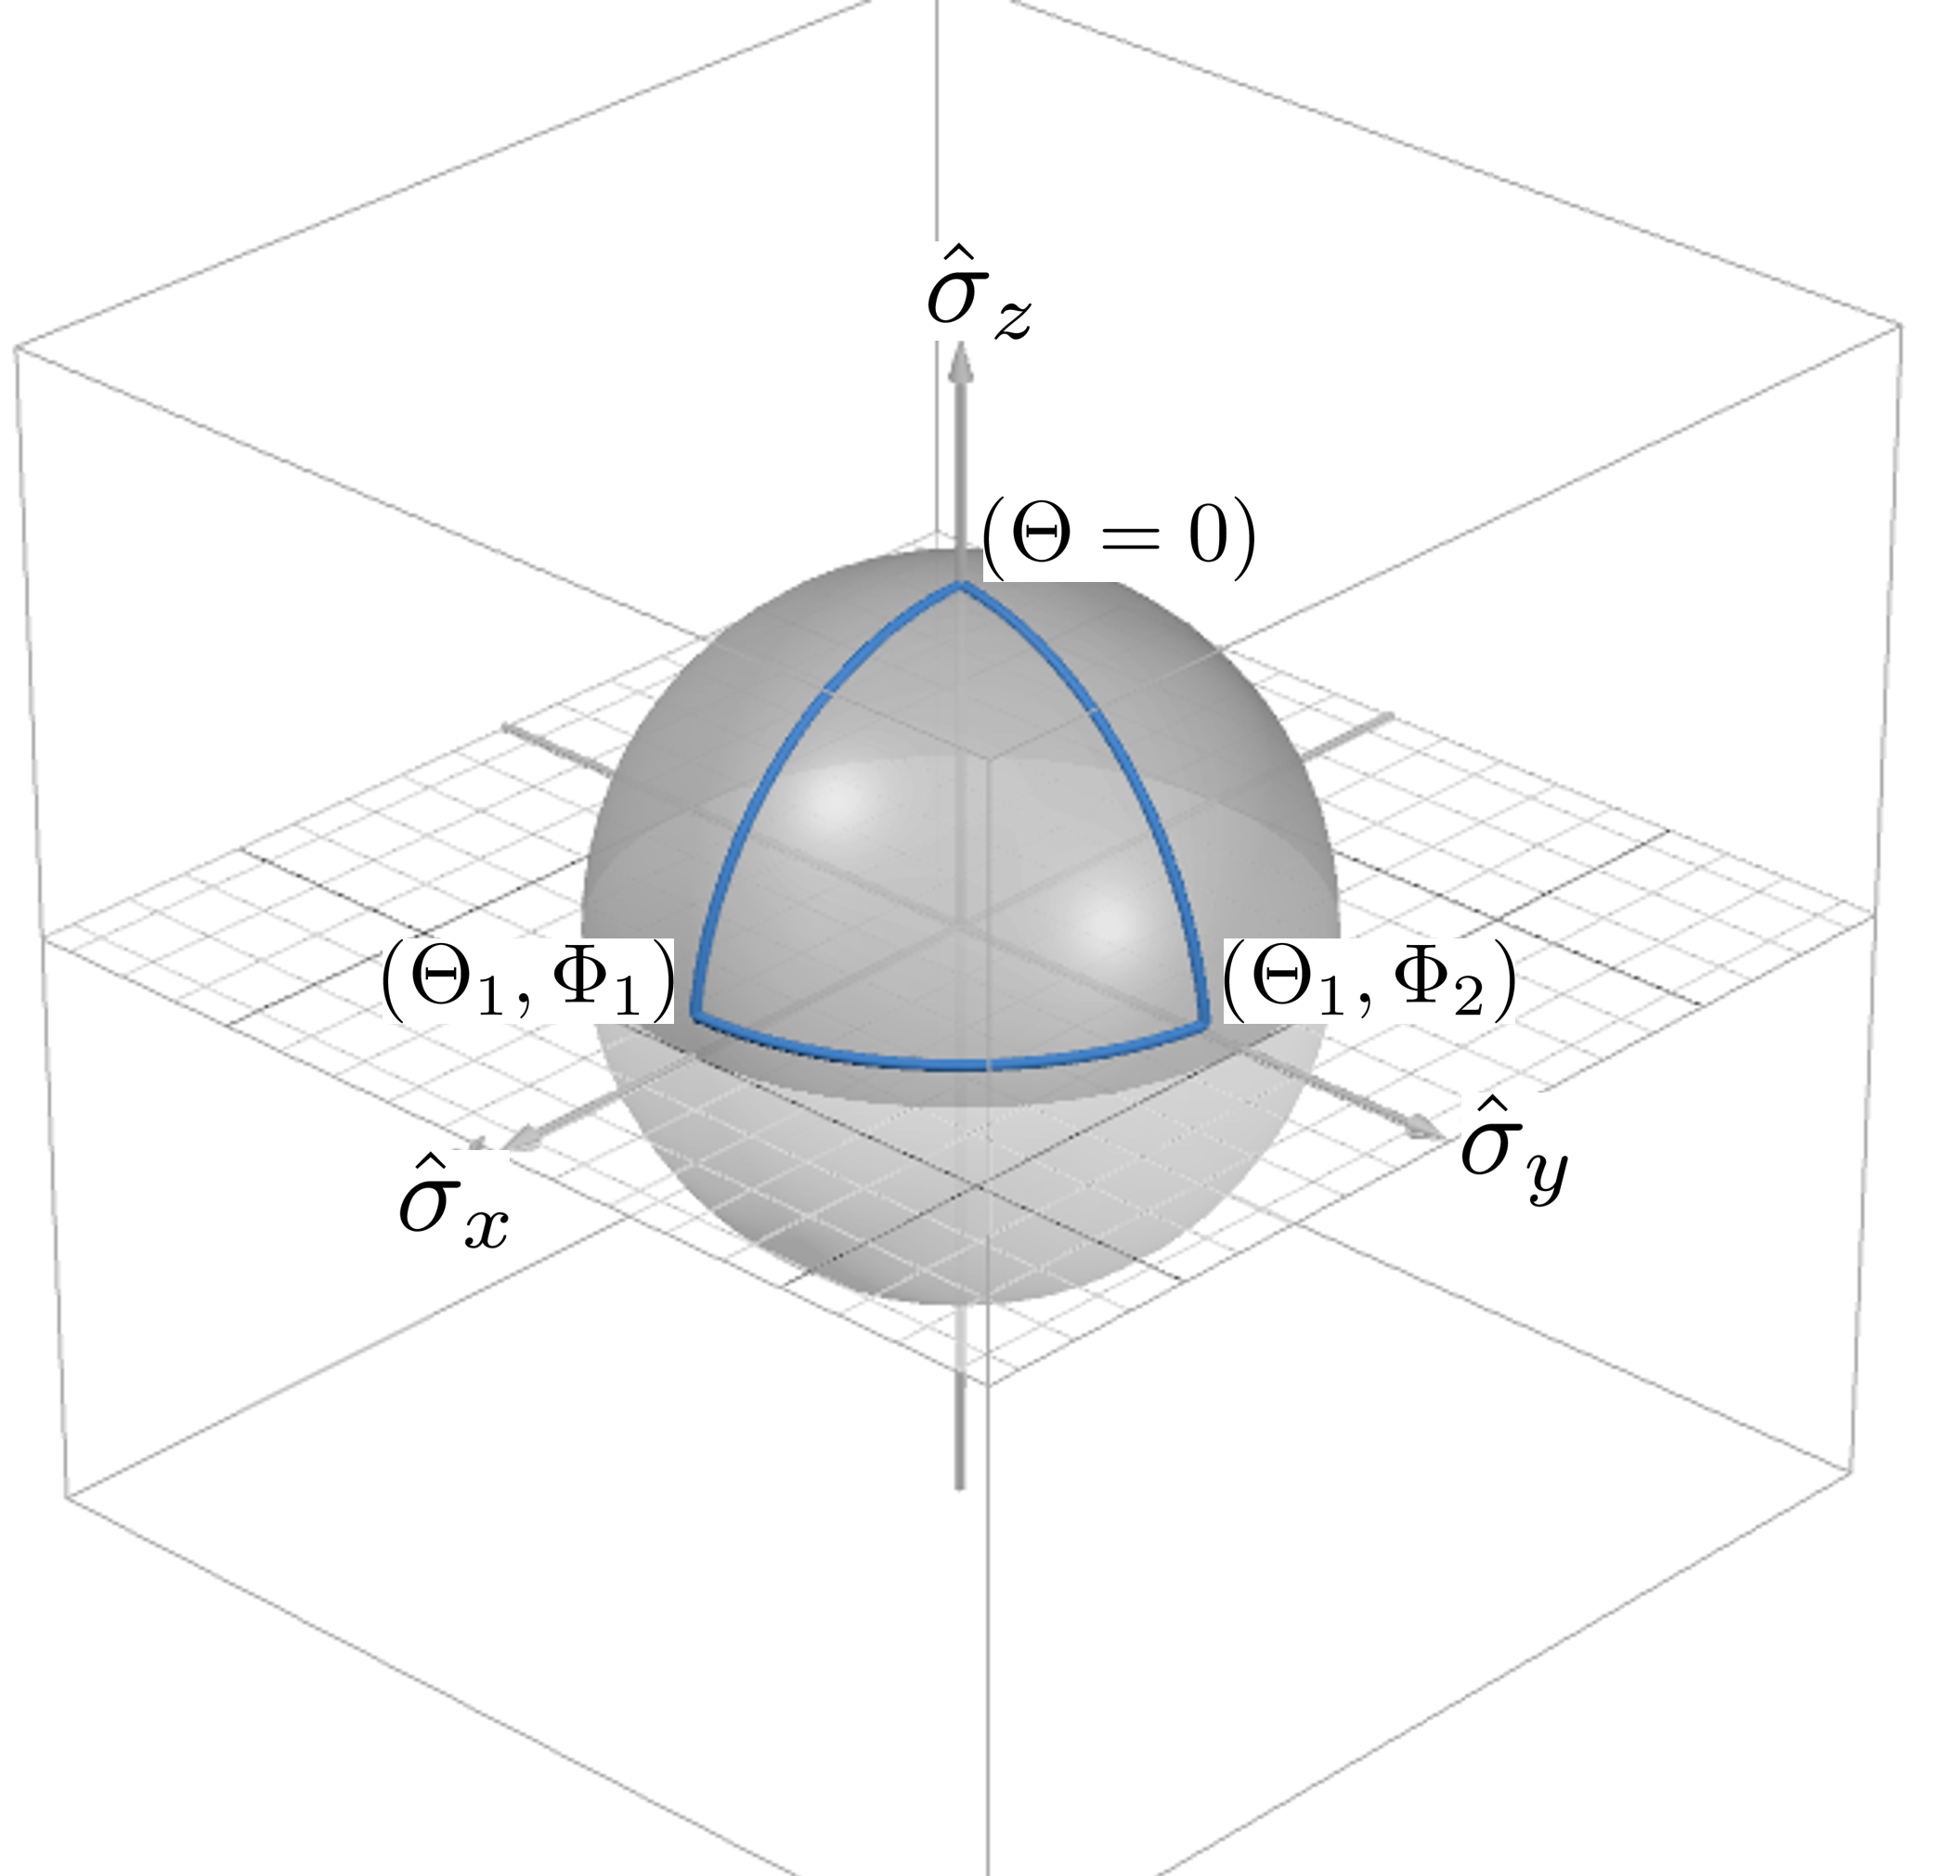
\includegraphics[scale=0.5]{figures/AAP_1.png}
  \caption{分極ベクトル$\bm{p}$の経路}
  \label{fig:AAP_1}
\end{figure}

\begin{figure}[htbp]
  \centering
  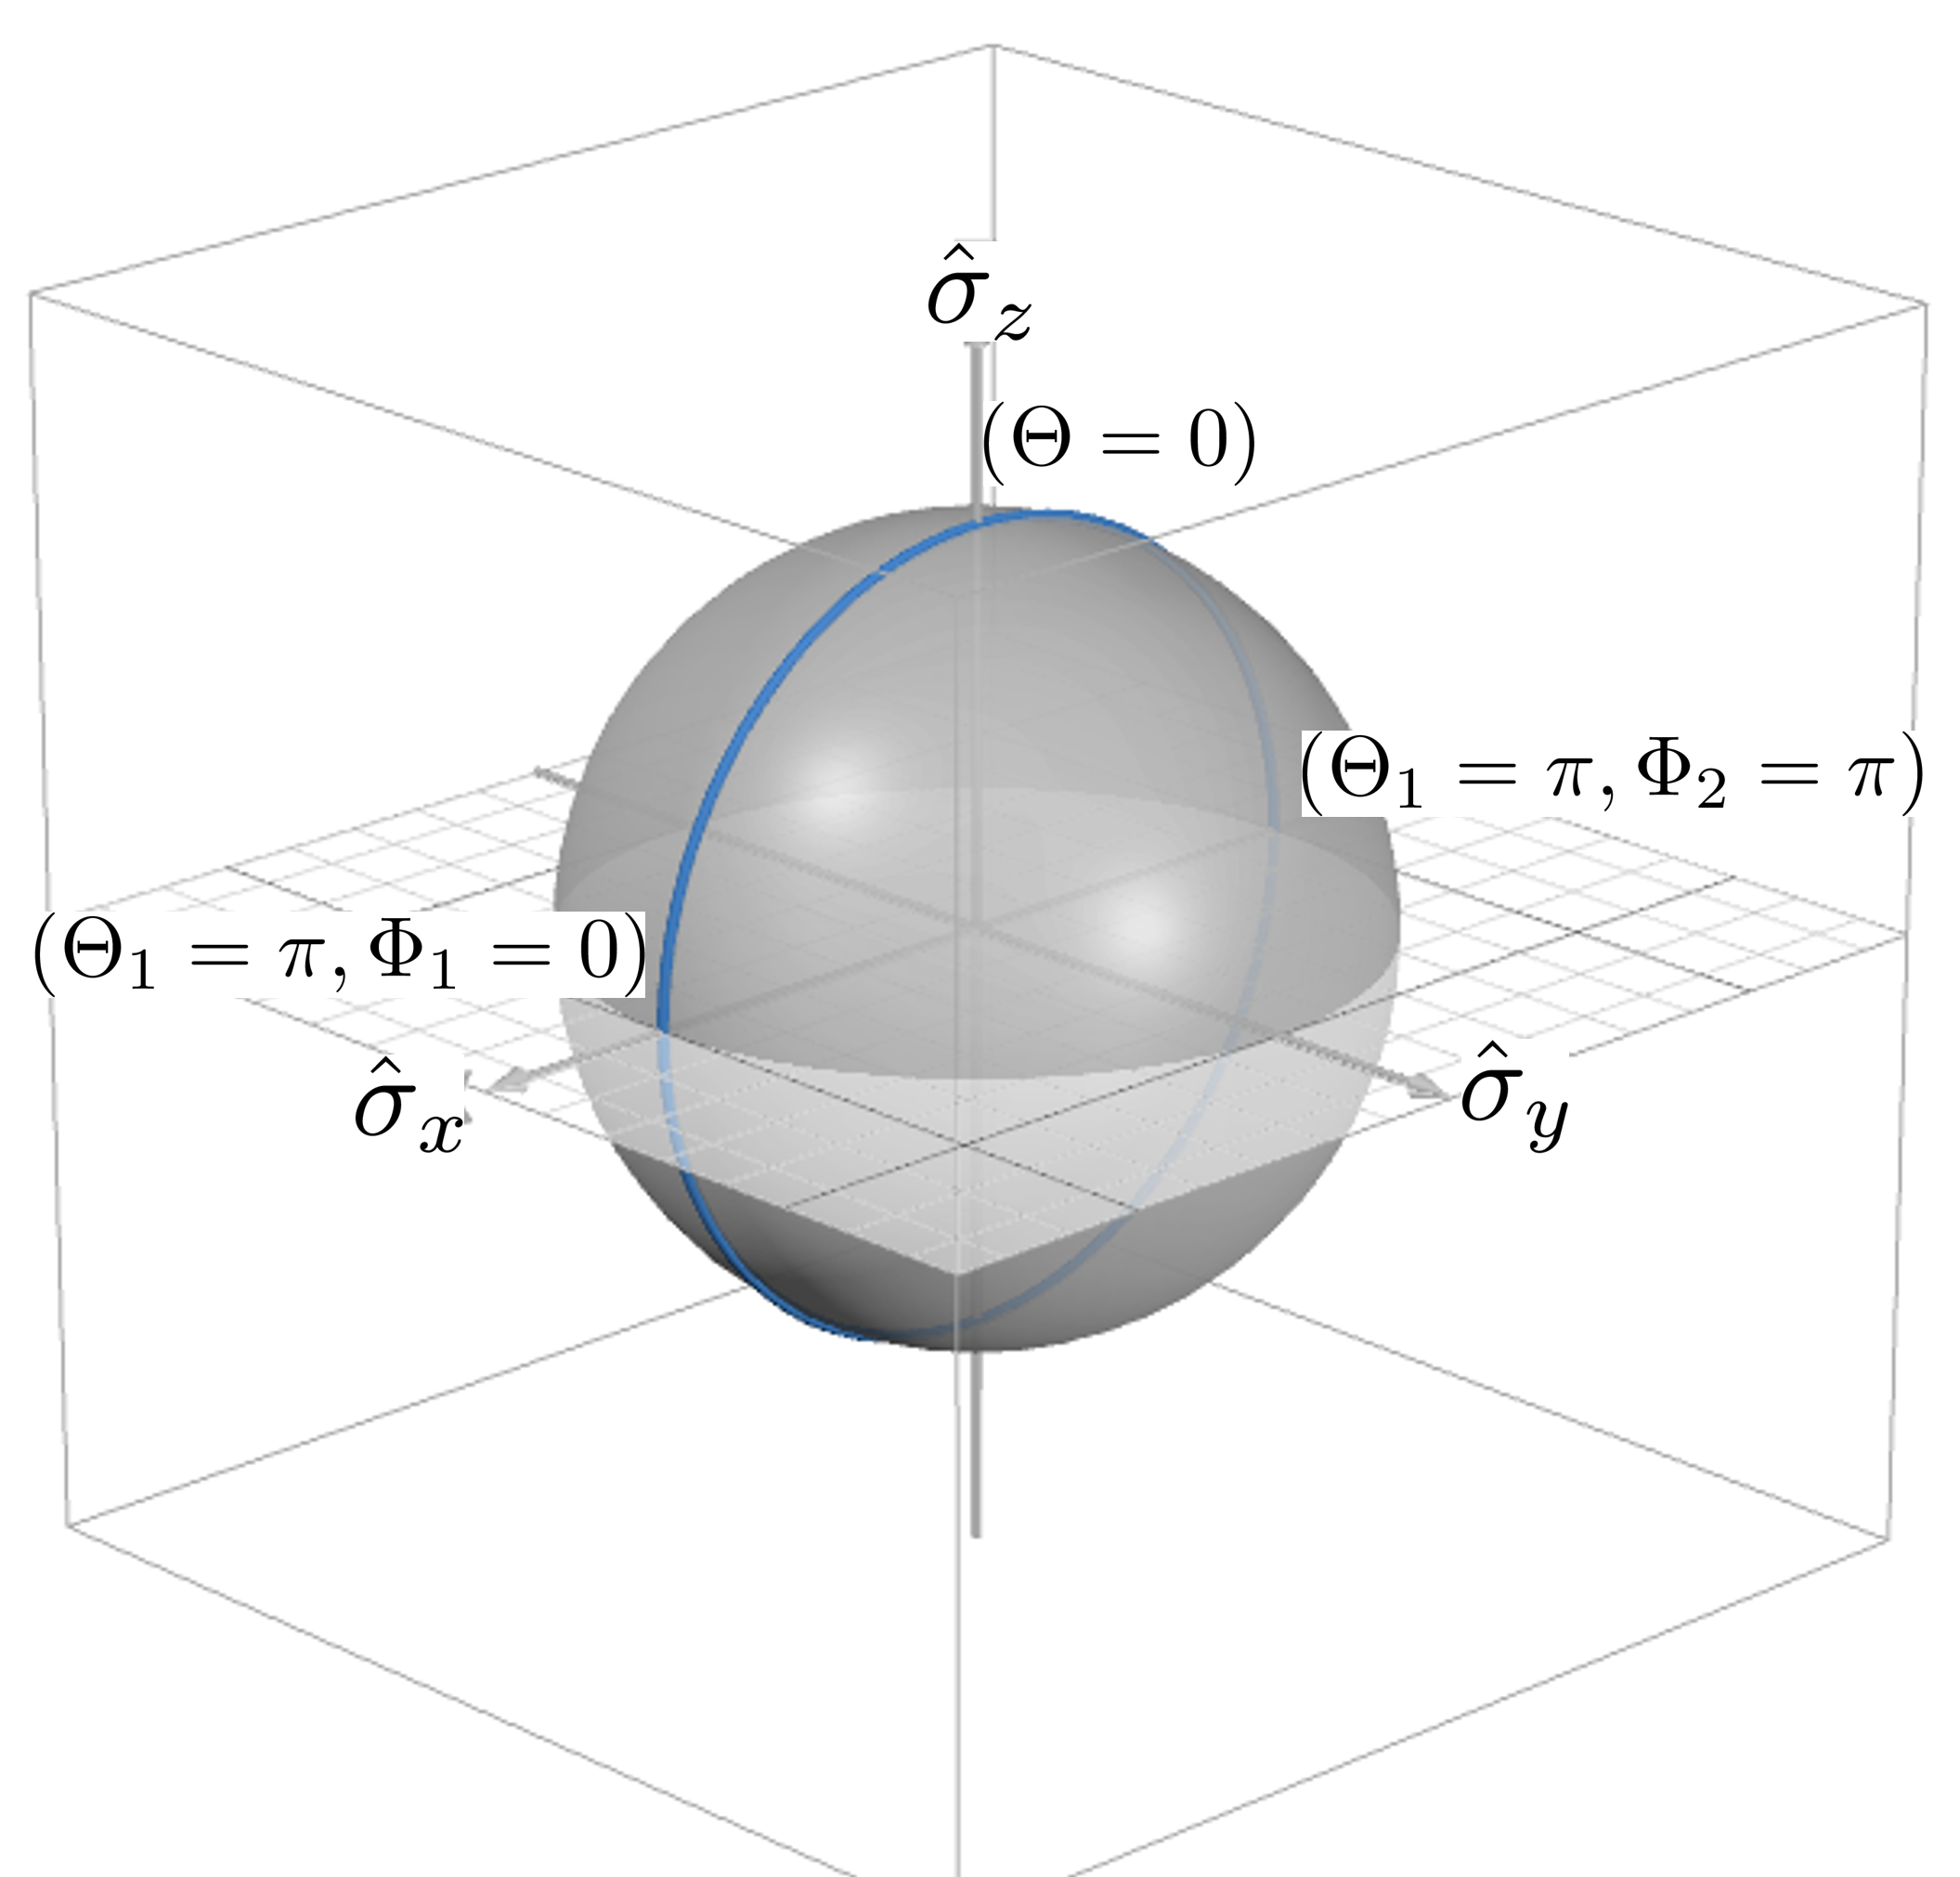
\includegraphics[scale=0.5]{figures/AAP_2.png}
  \caption{断熱極限における,分極ベクトル$\bm{p}$の経路}
  \label{fig:AAP_2}
\end{figure}


最後に,$2n$回目の準位交差で初期状態に戻る一般的な場合について,Aharonov-Anandan位相を求めておこう.式(\ref{cos_xi})で定義される$\xi$が,
\begin{equation}
  \xi = \frac{l}{2n} \pi \quad (l,n \text{は互いに素で,}0 < l < 2n) \label{xi_condition}
\end{equation}
のとき,$2n$回目の準位交差で,波動関数は符号を除いて初期状態に戻る.このことを確かめたければ,条件(\ref{xi_condition})を仮定して,式(\ref{psi_2m})を具体的に計算すればよい.


では,$2$回目の準位交差でAharonov-Ahandan位相を求めたときに用いた方法のように,まず動力学的位相から求めよう.系を4つの領域
\begin{enumerate}
\setcounter{enumi}{3}
\renewcommand{\labelenumi}{(\roman{enumi})}
  \item $t=0$から$t = \frac{\pi}{2\omega}$までの区間
  \item $t= \frac{\pi + 4k\pi}{2\omega}$から$t = \frac{3\pi + 4k\pi}{2\omega}$までの区間
  \item $t = \frac{3\pi + 4k\pi}{2\omega}$から$t = \frac{4\pi + 5k\pi}{2\omega}$までの区間 
  \item 最後のTLZ遷移から$t = \frac{2m\pi}{\omega}$までの区間
\end{enumerate}
に分割する.また,各領域における波動関数および動力学的位相をそれぞれ$\chi_d^{(\mathrm{x})}, \psi^{(\mathrm{x})} (\mathrm{x} = \mathrm{iv}, \mathrm{v}, \mathrm{vi}, \mathrm{vii})$とする.このとき,(iv)および(vii)の領域における動力学的位相は,$2$回目の準位交差でAharonov-Ahandan位相を求めたときと同様に,それぞれ$-\theta/2$である.また,(v)$t= \frac{\pi + 4k\pi}{2\omega}$から$t = \frac{3\pi + 4k\pi}{2\omega}$のときの動力学的位相$\chi_d^{(\mathrm{v})}$は,
\begin{align}
  -\left( 1 - 2q \left( \frac{\sin (2m-1) \xi}{\sin \xi} \right)^2 \right) \theta,
\end{align}
(vi)$t = \frac{3\pi + 4k\pi}{2\omega}$から$t = \frac{4\pi + 5k\pi}{2\omega}$のときの動力学的位相$\chi_d^{(\mathrm{vi})}$は,
\begin{align}
  -\left( 1 - 2q \left( \frac{\sin (2m) \xi}{\sin \xi}\right)^2\right) \theta,
\end{align}
であることが,$2$回目の準位交差でAharonov-Ahandan位相を求めたときと同様に計算できる.


したがって,
\begin{align}
  \chi_d
  &= - \theta - \sum_{m=1}^{2n-1} \left( 1 - 2q \left(\frac{\sin (2m) \xi}{\sin \xi}\right)^2\right) \theta\\
  &= -\theta - (2n-1) \theta + 2nq\frac{1}{\sin^2 \xi}\\
  &= -2n\theta (1-\frac{q}{\sin^2 \xi})
\end{align}
より,$2n$回目の準位交差で初期状態に戻る一般的な場合におけるAharonov-Anandan位相は,
\begin{equation}
  \chi_g = (n+l)\pi + 2n\theta \left( 1-\frac{q}{\sin^2 \xi} \right)
\end{equation}
である.$n=1$を代入すると,明らかに式(\ref{chi_g_AA})に一致する.

\chapter{TLZ遷移を含むcyclic evolution}
第\ref{NT}章で,測地曲率がTwisted Landau-Zener遷移の確率に影響を及ぼすことを確認した.また,第\ref{CE}章で,Landau-Zener遷移を含むcyclic evolutionモデルにおいて,波動関数の干渉がさまざまな現象を引き起こすことを確認した.本章では,これら2つのモデルを組み合わせることによって,波動関数の干渉と測地曲率が織りなす現象が見られることを示す.

\section{整流作用を取り入れた系}

\subsection{モデルの解説}
TLZ遷移を含むcyclic evolutionに整流作用を取り入れた系におけるHamiltonianは
\begin{equation}
  \Hat{H} = \Delta_0 \sin \omega t \, \Hat{\sigma}_x +\frac{1}{4} \kappa_g \varepsilon_0^2 \cos \omega t \sin 2 \omega t \, \Hat{\sigma}_y + \varepsilon_0 \cos \omega t \, \Hat{\sigma}_z \label{TLZ_CE}
\end{equation}
である.この系における断熱エネルギーの時間変化は図\ref{fig:CEwithTLZ}のようになる.初期状態が$|2\rangle$であるとき,1番目のTLZ遷移で2つの経路に分かれる.その後,2番目以降のTLZ遷移で2つの経路の干渉が生じる.


また,Pauli行列を基底とした空間に,このHamiltonianを描写すると図\ref{fig:TLZ_CE_Pauli_1}から図\ref{fig:TLZ_CE_Pauli_3}のようになる.図\ref{fig:TLZ_CE_Pauli_1}から図\ref{fig:TLZ_CE_Pauli_3}より,この系のHamiltonianの経路は楕円を$y$軸方向にねじったような形をしている.そのため,この系はcyclic evolutionである.



\begin{figure}[htbp]
  \centering
  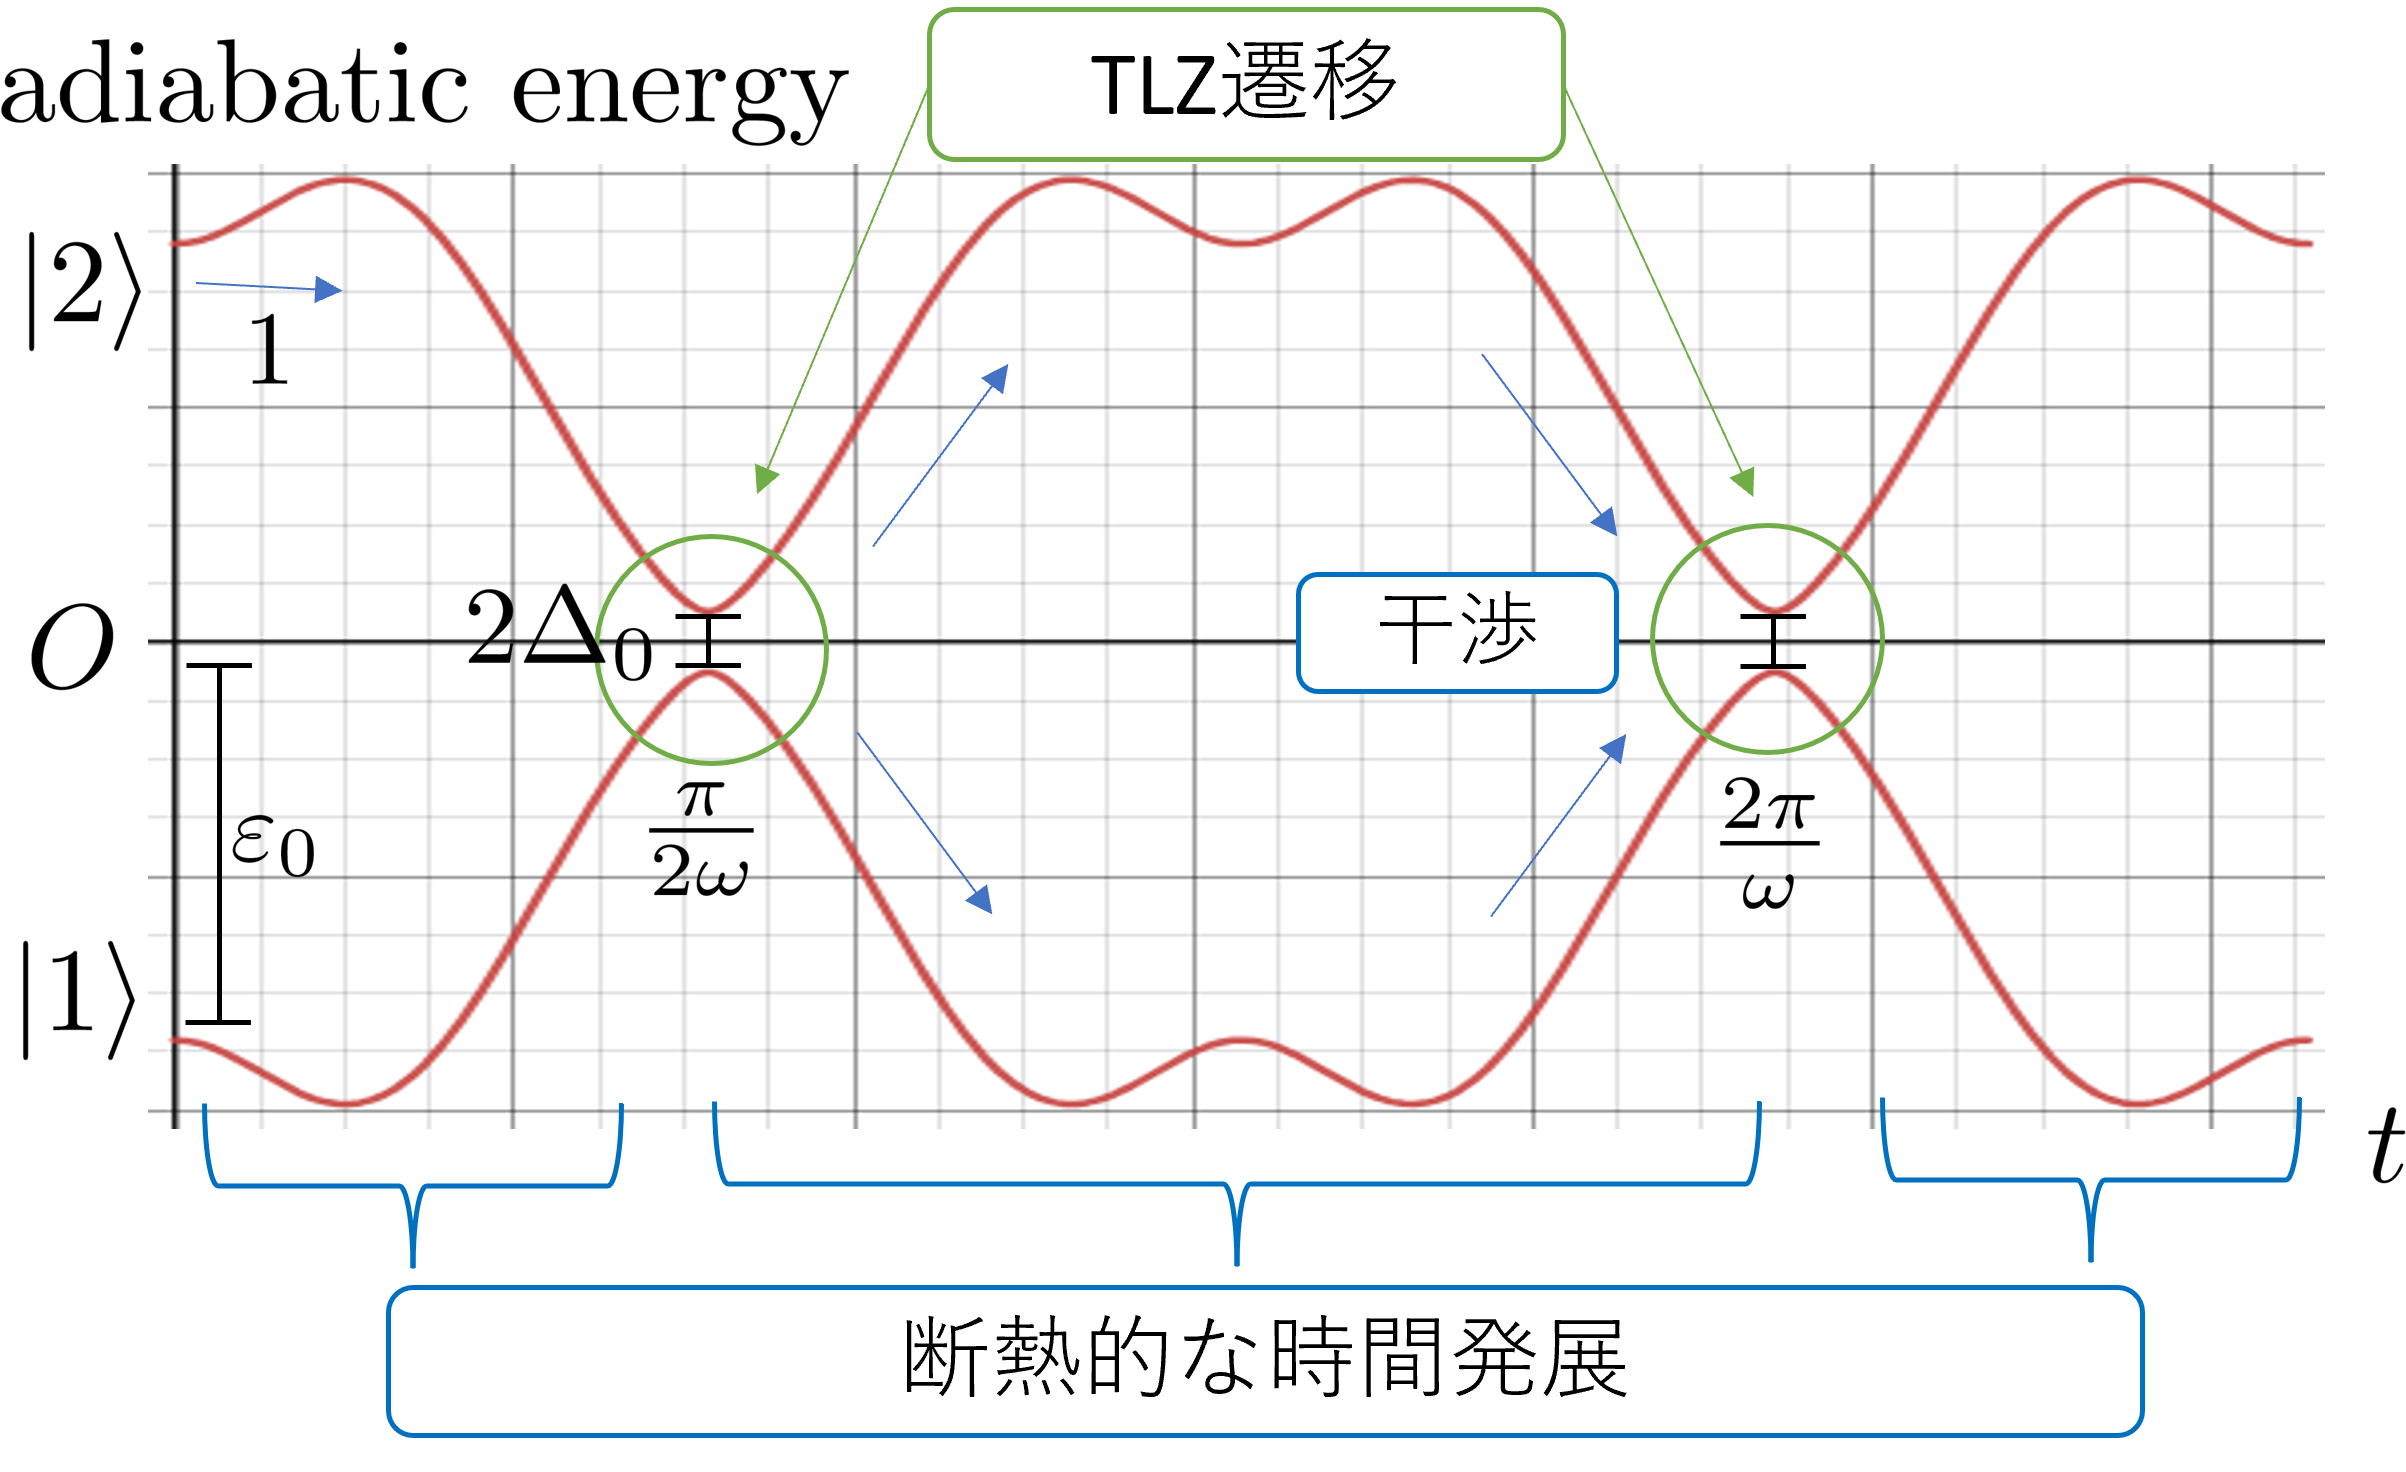
\includegraphics[scale=0.5]{figures/TLZ_CE.png}
  \caption{TLZ遷移を含むcyclic evolution(\ref{TLZ_CE})における断熱エネルギーの時間変化}
  \label{fig:CEwithTLZ}
\end{figure}

\begin{figure}[htbp]
  \centering
  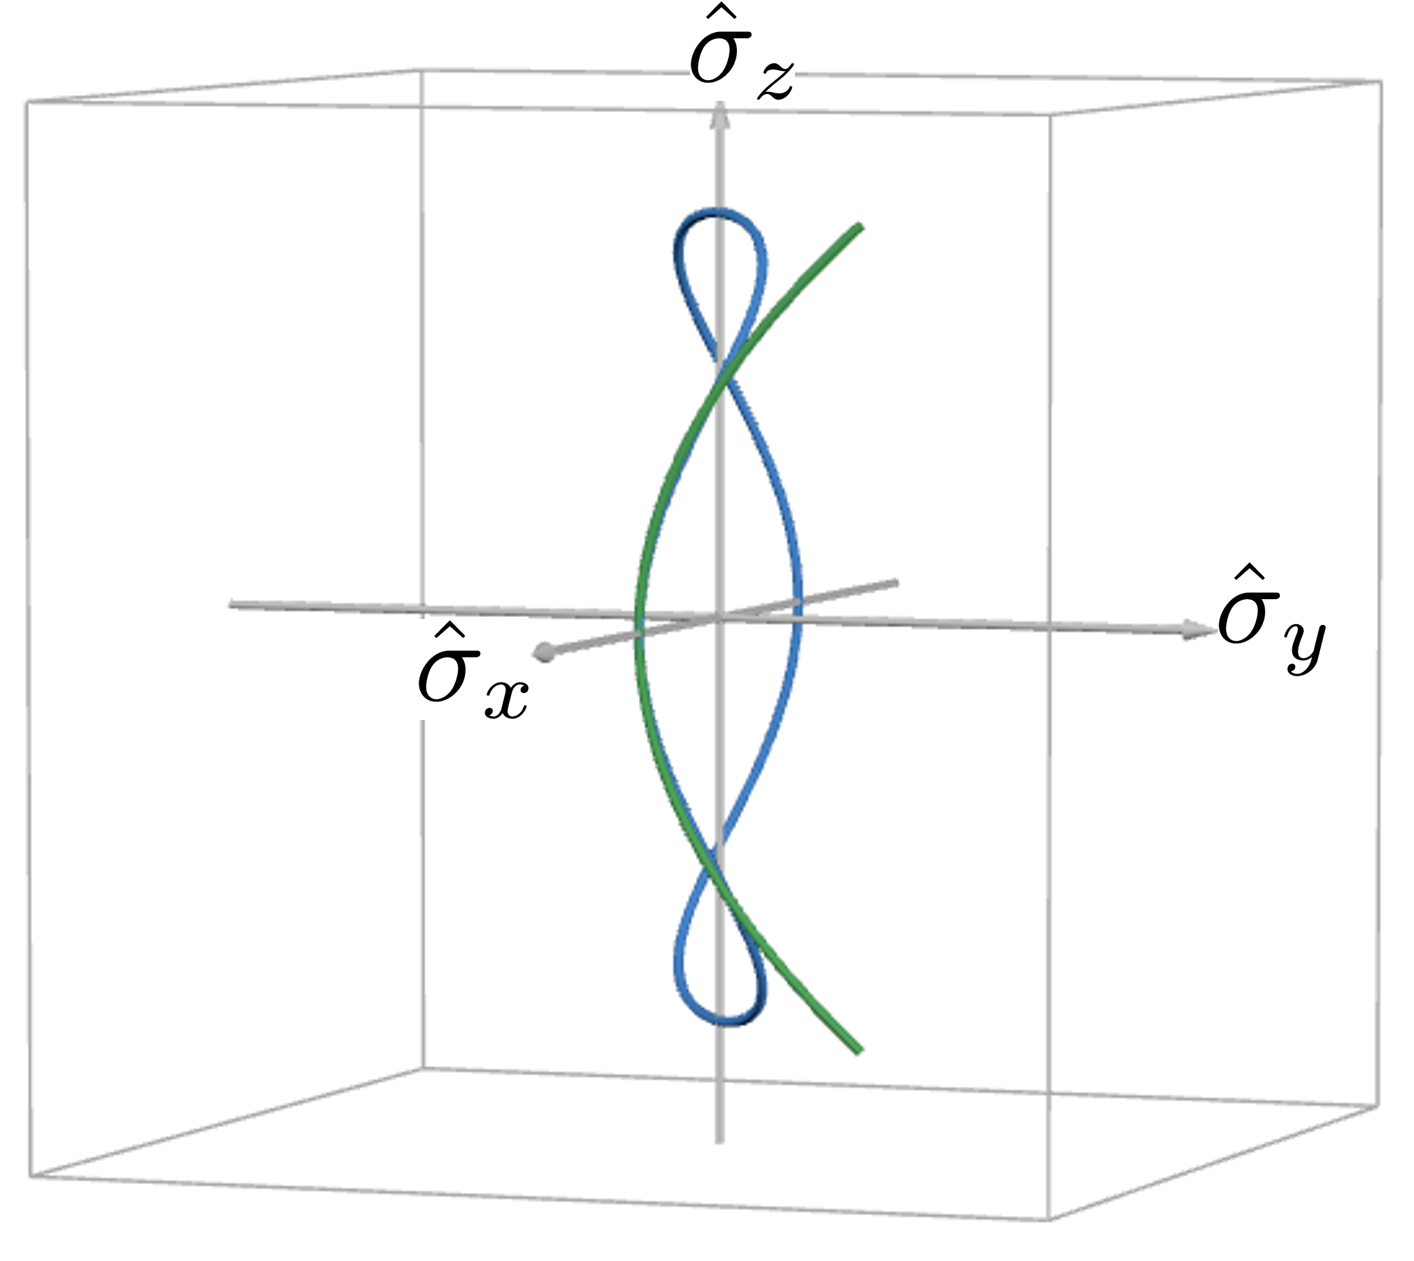
\includegraphics[scale=0.5]{figures/TLZ_CE_Pauli_1.png}
  \caption{TLZモデルを含むcyclic evolution(\ref{TLZ_CE})におけるHamiltonianの経路}
  \label{fig:TLZ_CE_Pauli_1}
\end{figure}

\begin{figure}[htbp]
  \centering
  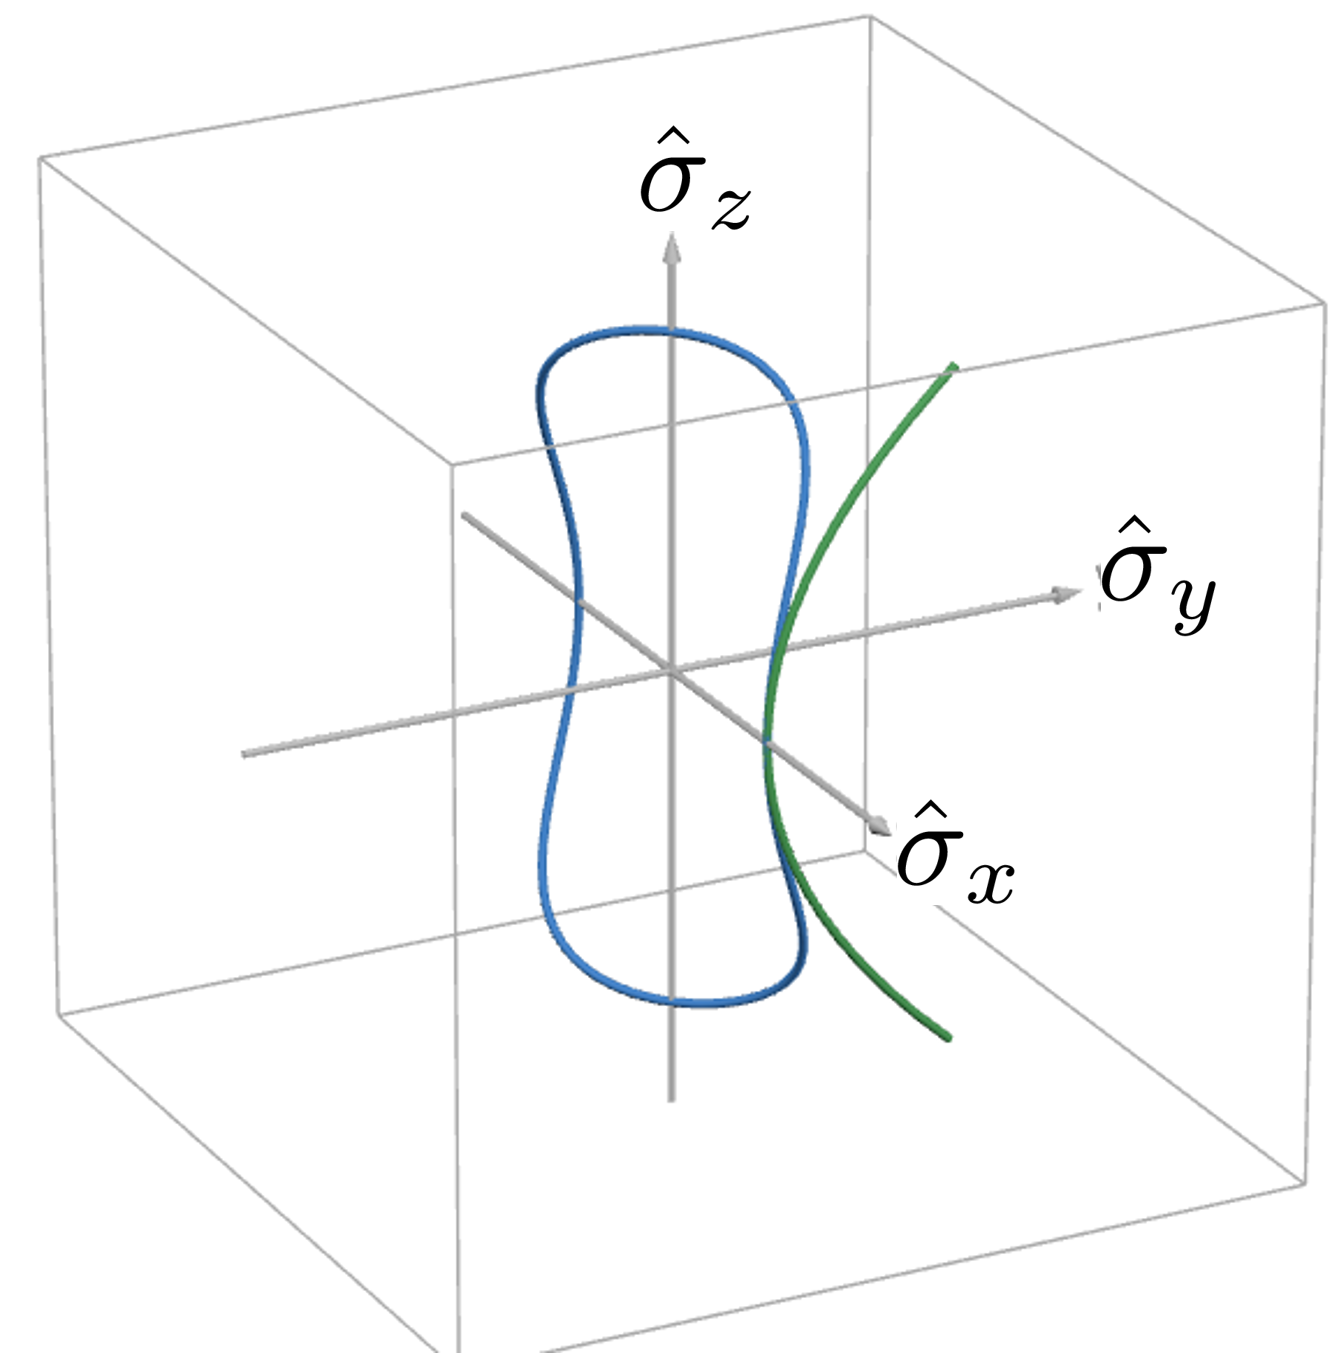
\includegraphics[scale=0.5]{figures/TLZ_CE_Pauli_2.png}
  \caption{TLZモデルを含むcyclic evolution(\ref{TLZ_CE})におけるHamiltonianの経路(別の角度からの視点)}
  \label{fig:TLZ_CE_Pauli_2}
\end{figure}

\begin{figure}[htbp]
  \centering
  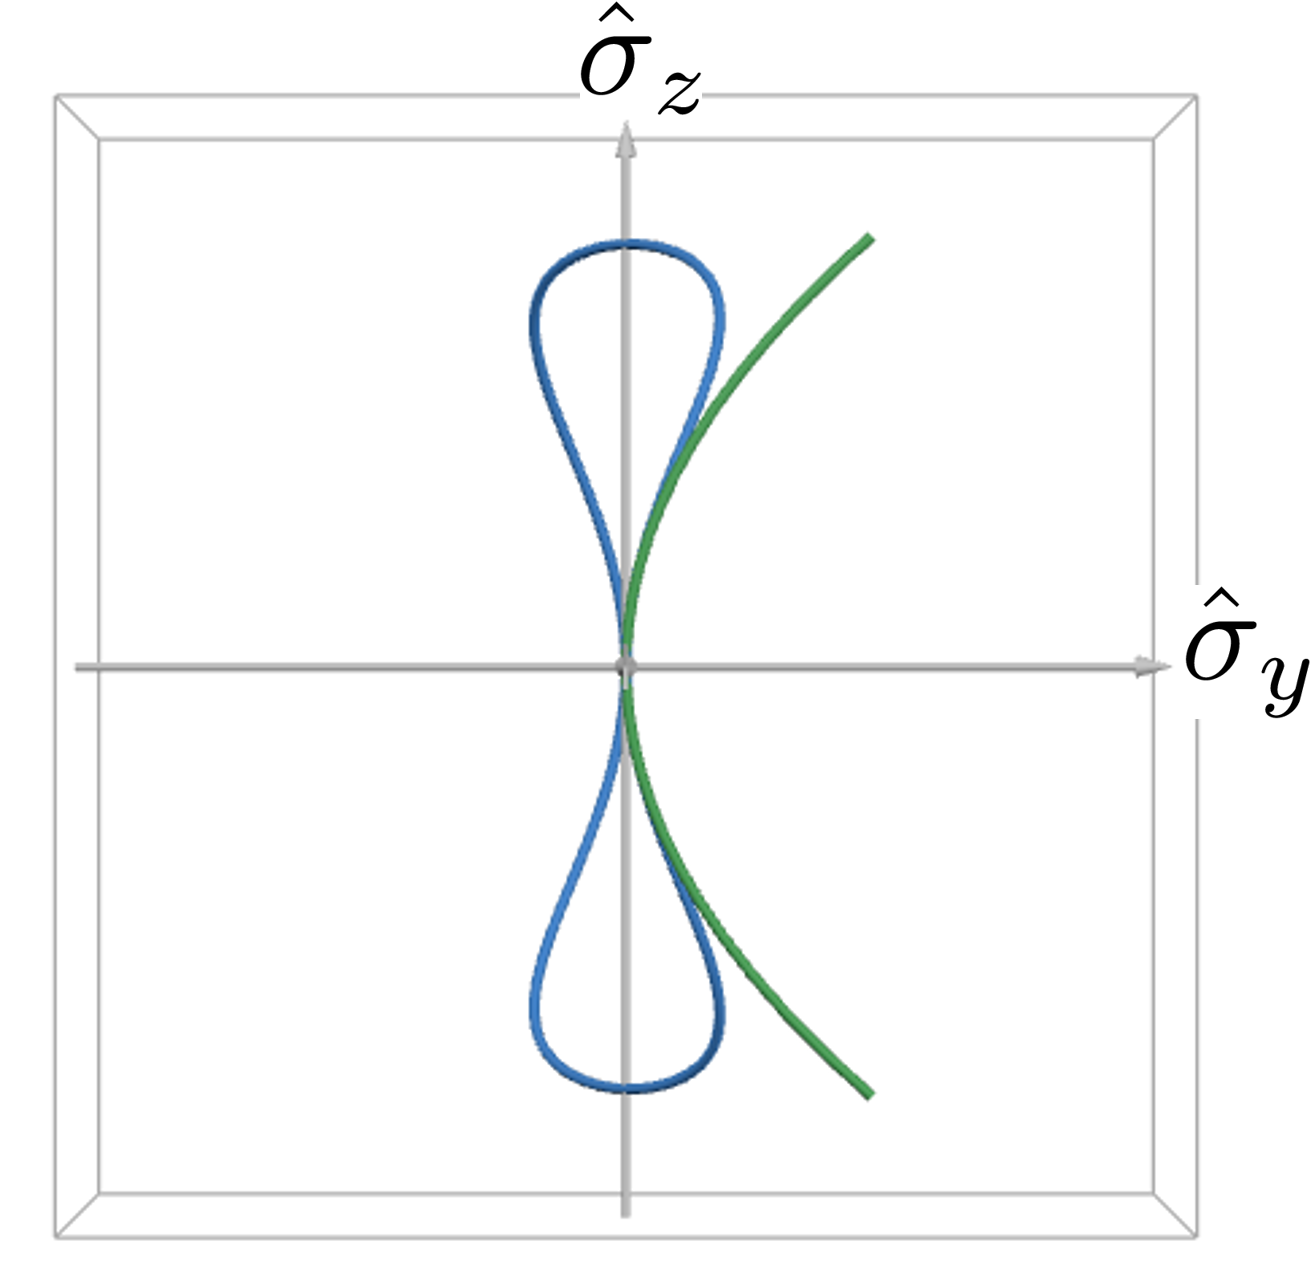
\includegraphics[scale=0.5]{figures/TLZ_CE_Pauli_5.png}
  \caption{TLZモデルを含むcyclic evolution(\ref{TLZ_CE})におけるHamiltonianの経路($x$軸視点)}
  \label{fig:TLZ_CE_Pauli_5}
\end{figure}

\begin{figure}[htbp]
  \centering
  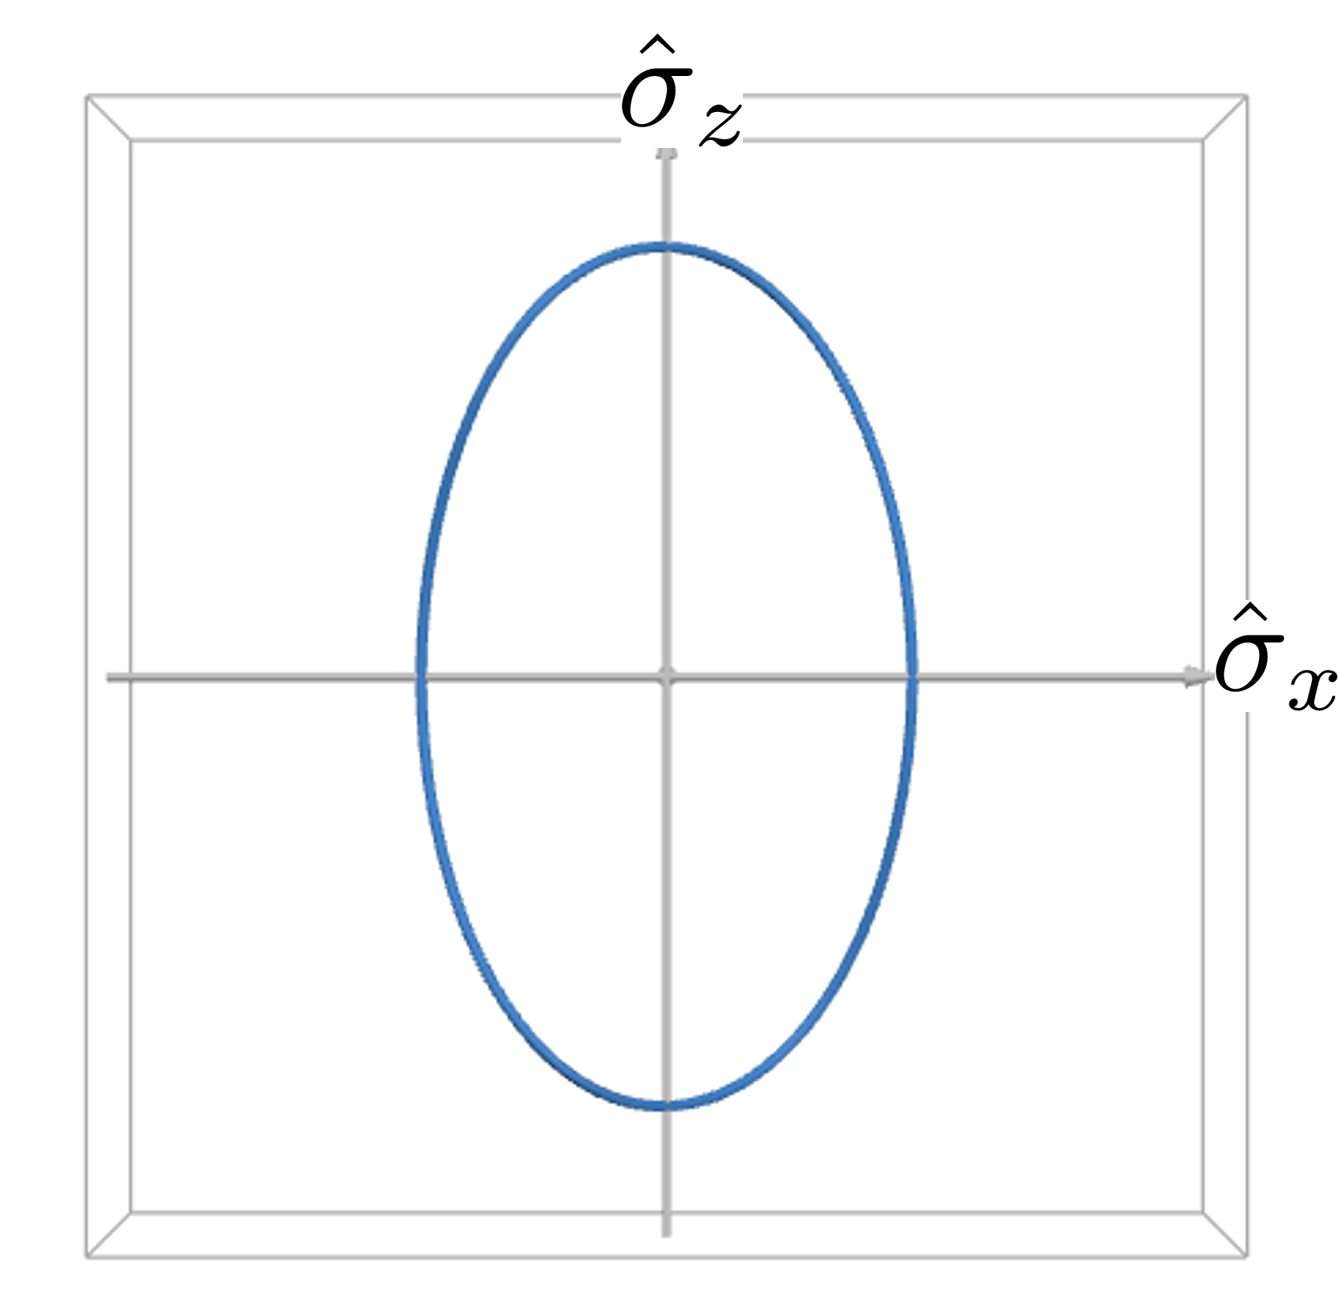
\includegraphics[scale=0.5]{figures/TLZ_CE_Pauli_4.png}
  \caption{TLZモデルを含むcyclic evolution(\ref{TLZ_CE})におけるHamiltonianの経路($y$軸視点)}
  \label{fig:TLZ_CE_Pauli_4}
\end{figure}

\begin{figure}[htbp]
  \centering
  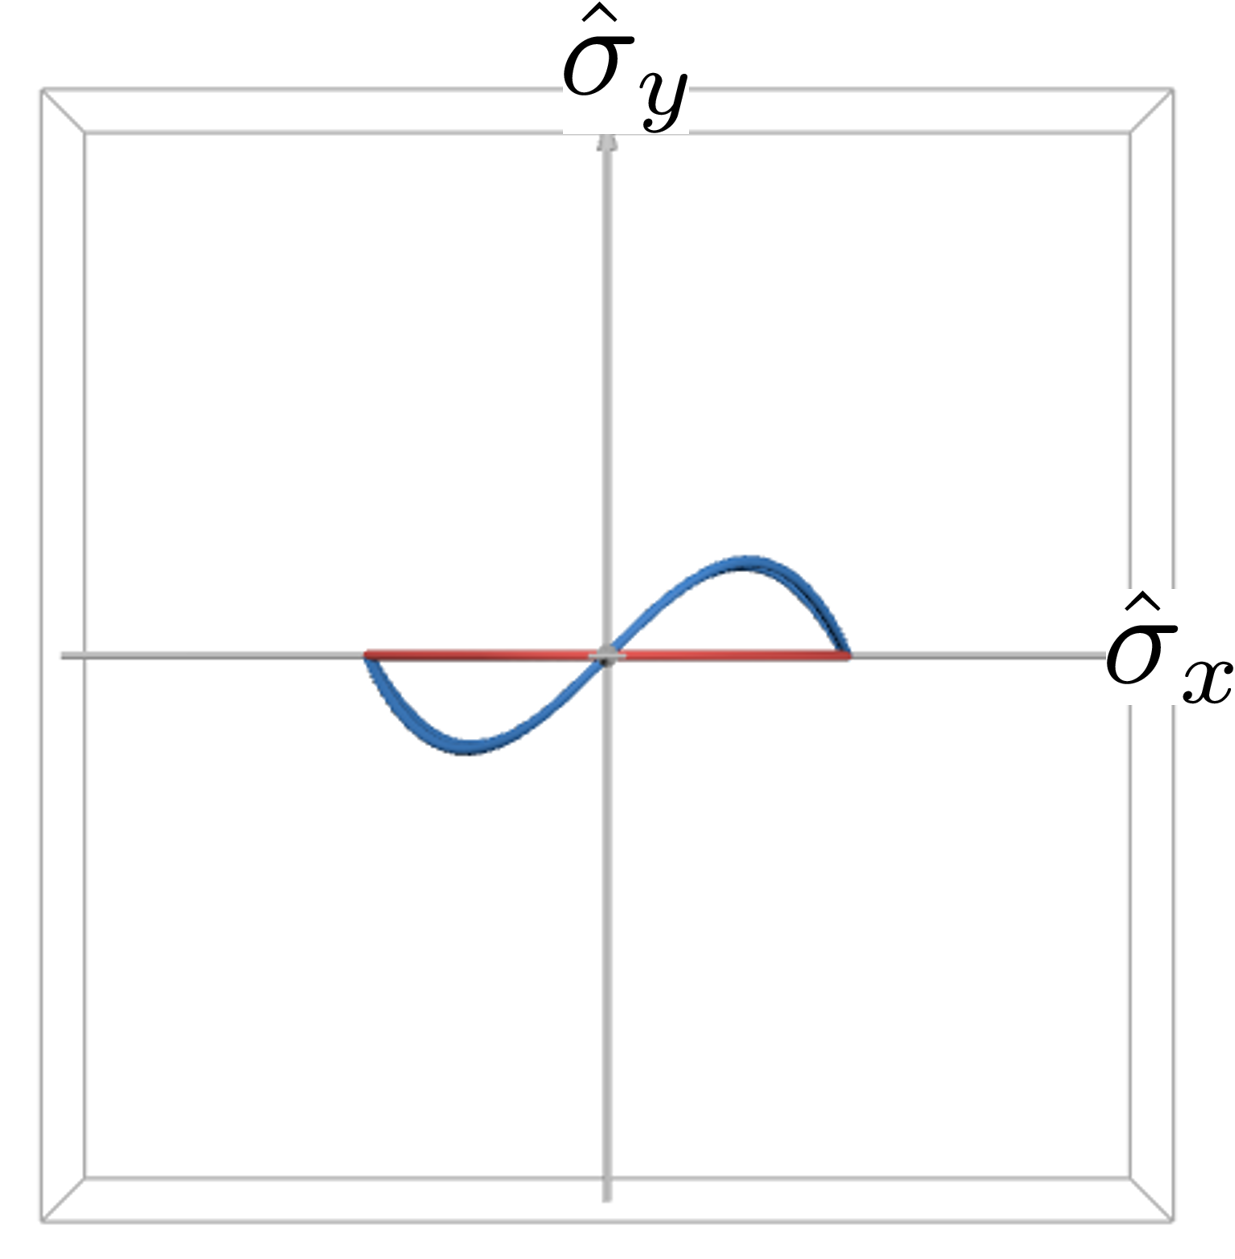
\includegraphics[scale=0.5]{figures/TLZ_CE_Pauli_3.png}
  \caption{TLZモデルを含むcyclic evolution(\ref{TLZ_CE})におけるHamiltonianの経路($z$軸視点)}
  \label{fig:TLZ_CE_Pauli_3}
\end{figure}





\subsection{数値計算の結果}
系が状態$|1\rangle$である確率($|1\rangle$ occupation probability)$P(t)$の時間変化を$\kappa_g=0.27$および$\kappa_g=0$としてそれぞれプロットすると図\ref{fig:NR_k}および図\ref{fig:NR_k=0}のようになる.


図\ref{fig:NR_k=0}では,各遷移ごとに状態の占有確率が変化する.一方,図\ref{fig:NR_k}では,2回の遷移ごとに占有確率が変化している.この現象は,完全トンネルおよび整流作用によって引き起こされると考えられる.4回目の遷移では,波動関数の干渉と測地曲率の2つの要因によって状態の占有確率が決定されていると考えられるが,詳しくはわかっていない.

\begin{figure}[htbp]
  \centering
  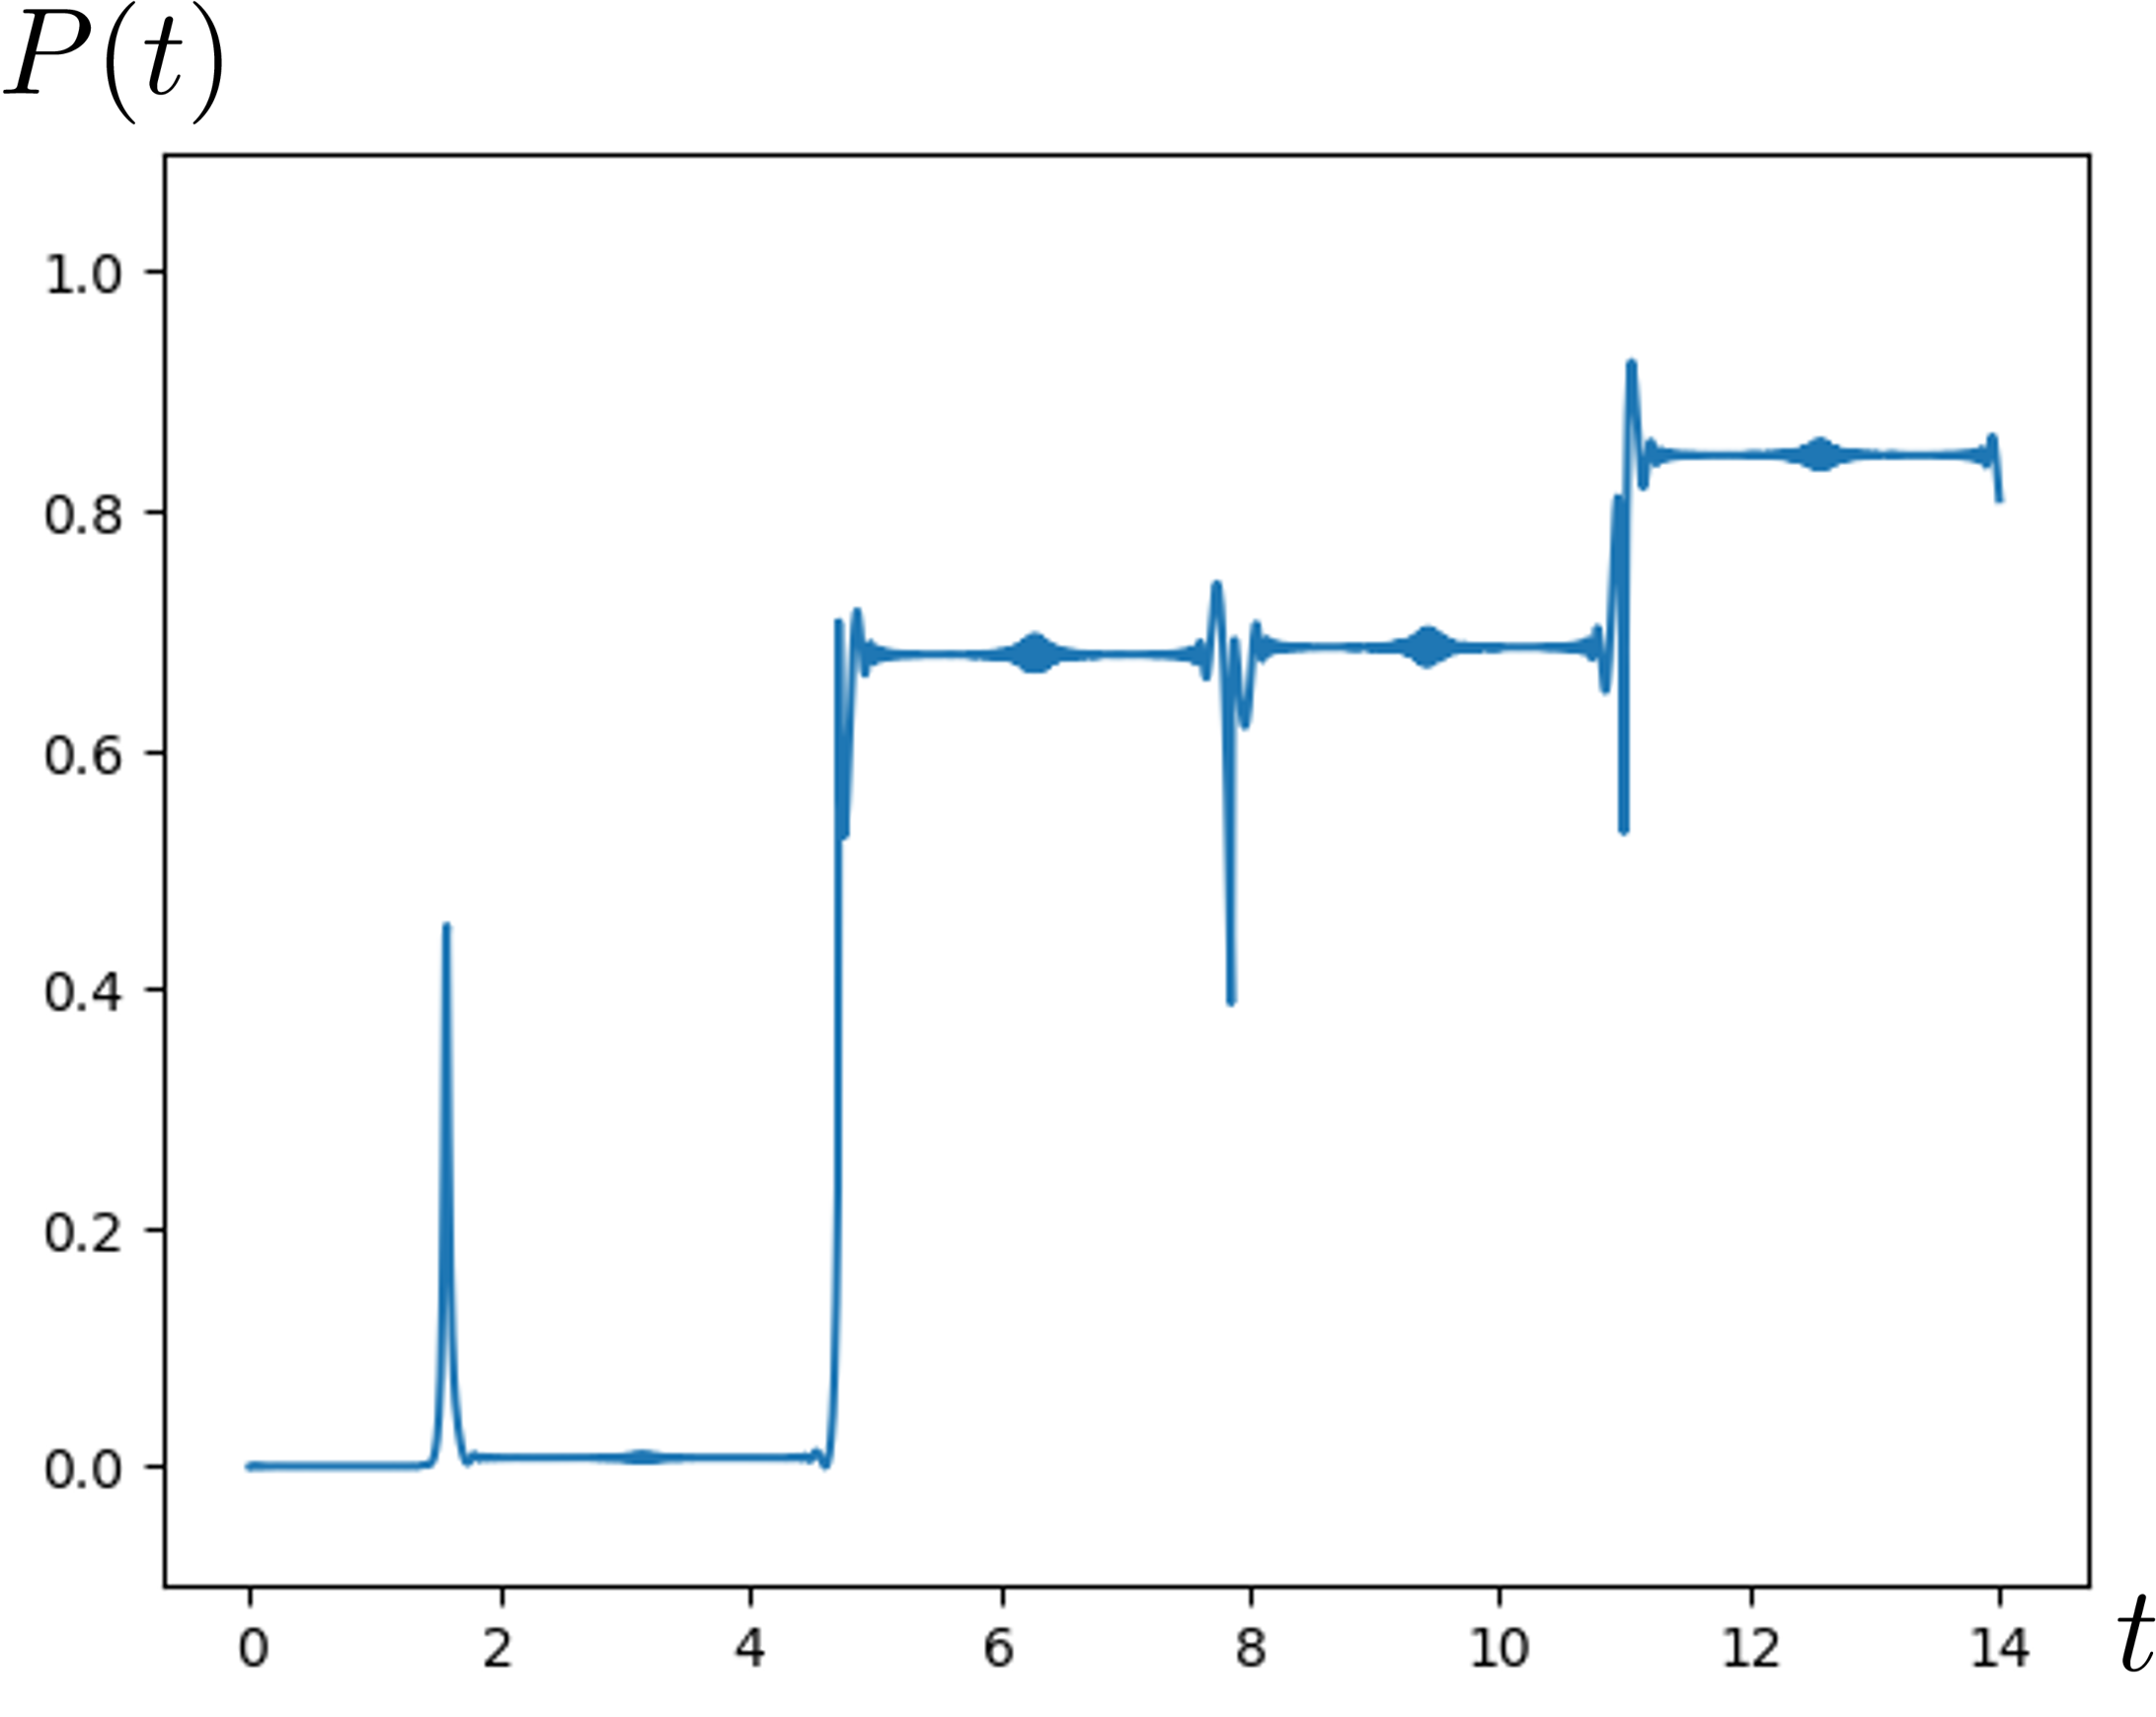
\includegraphics[scale=0.5]{figures/k_0.27.png}
  \caption{$\kappa_g=0.27$における$P(t)$の時間変化.$\varepsilon_0=90, \Delta_0 = 3, \omega=1$とした.}
  \label{fig:NR_k}
\end{figure}

\begin{figure}[htbp]
  \centering
  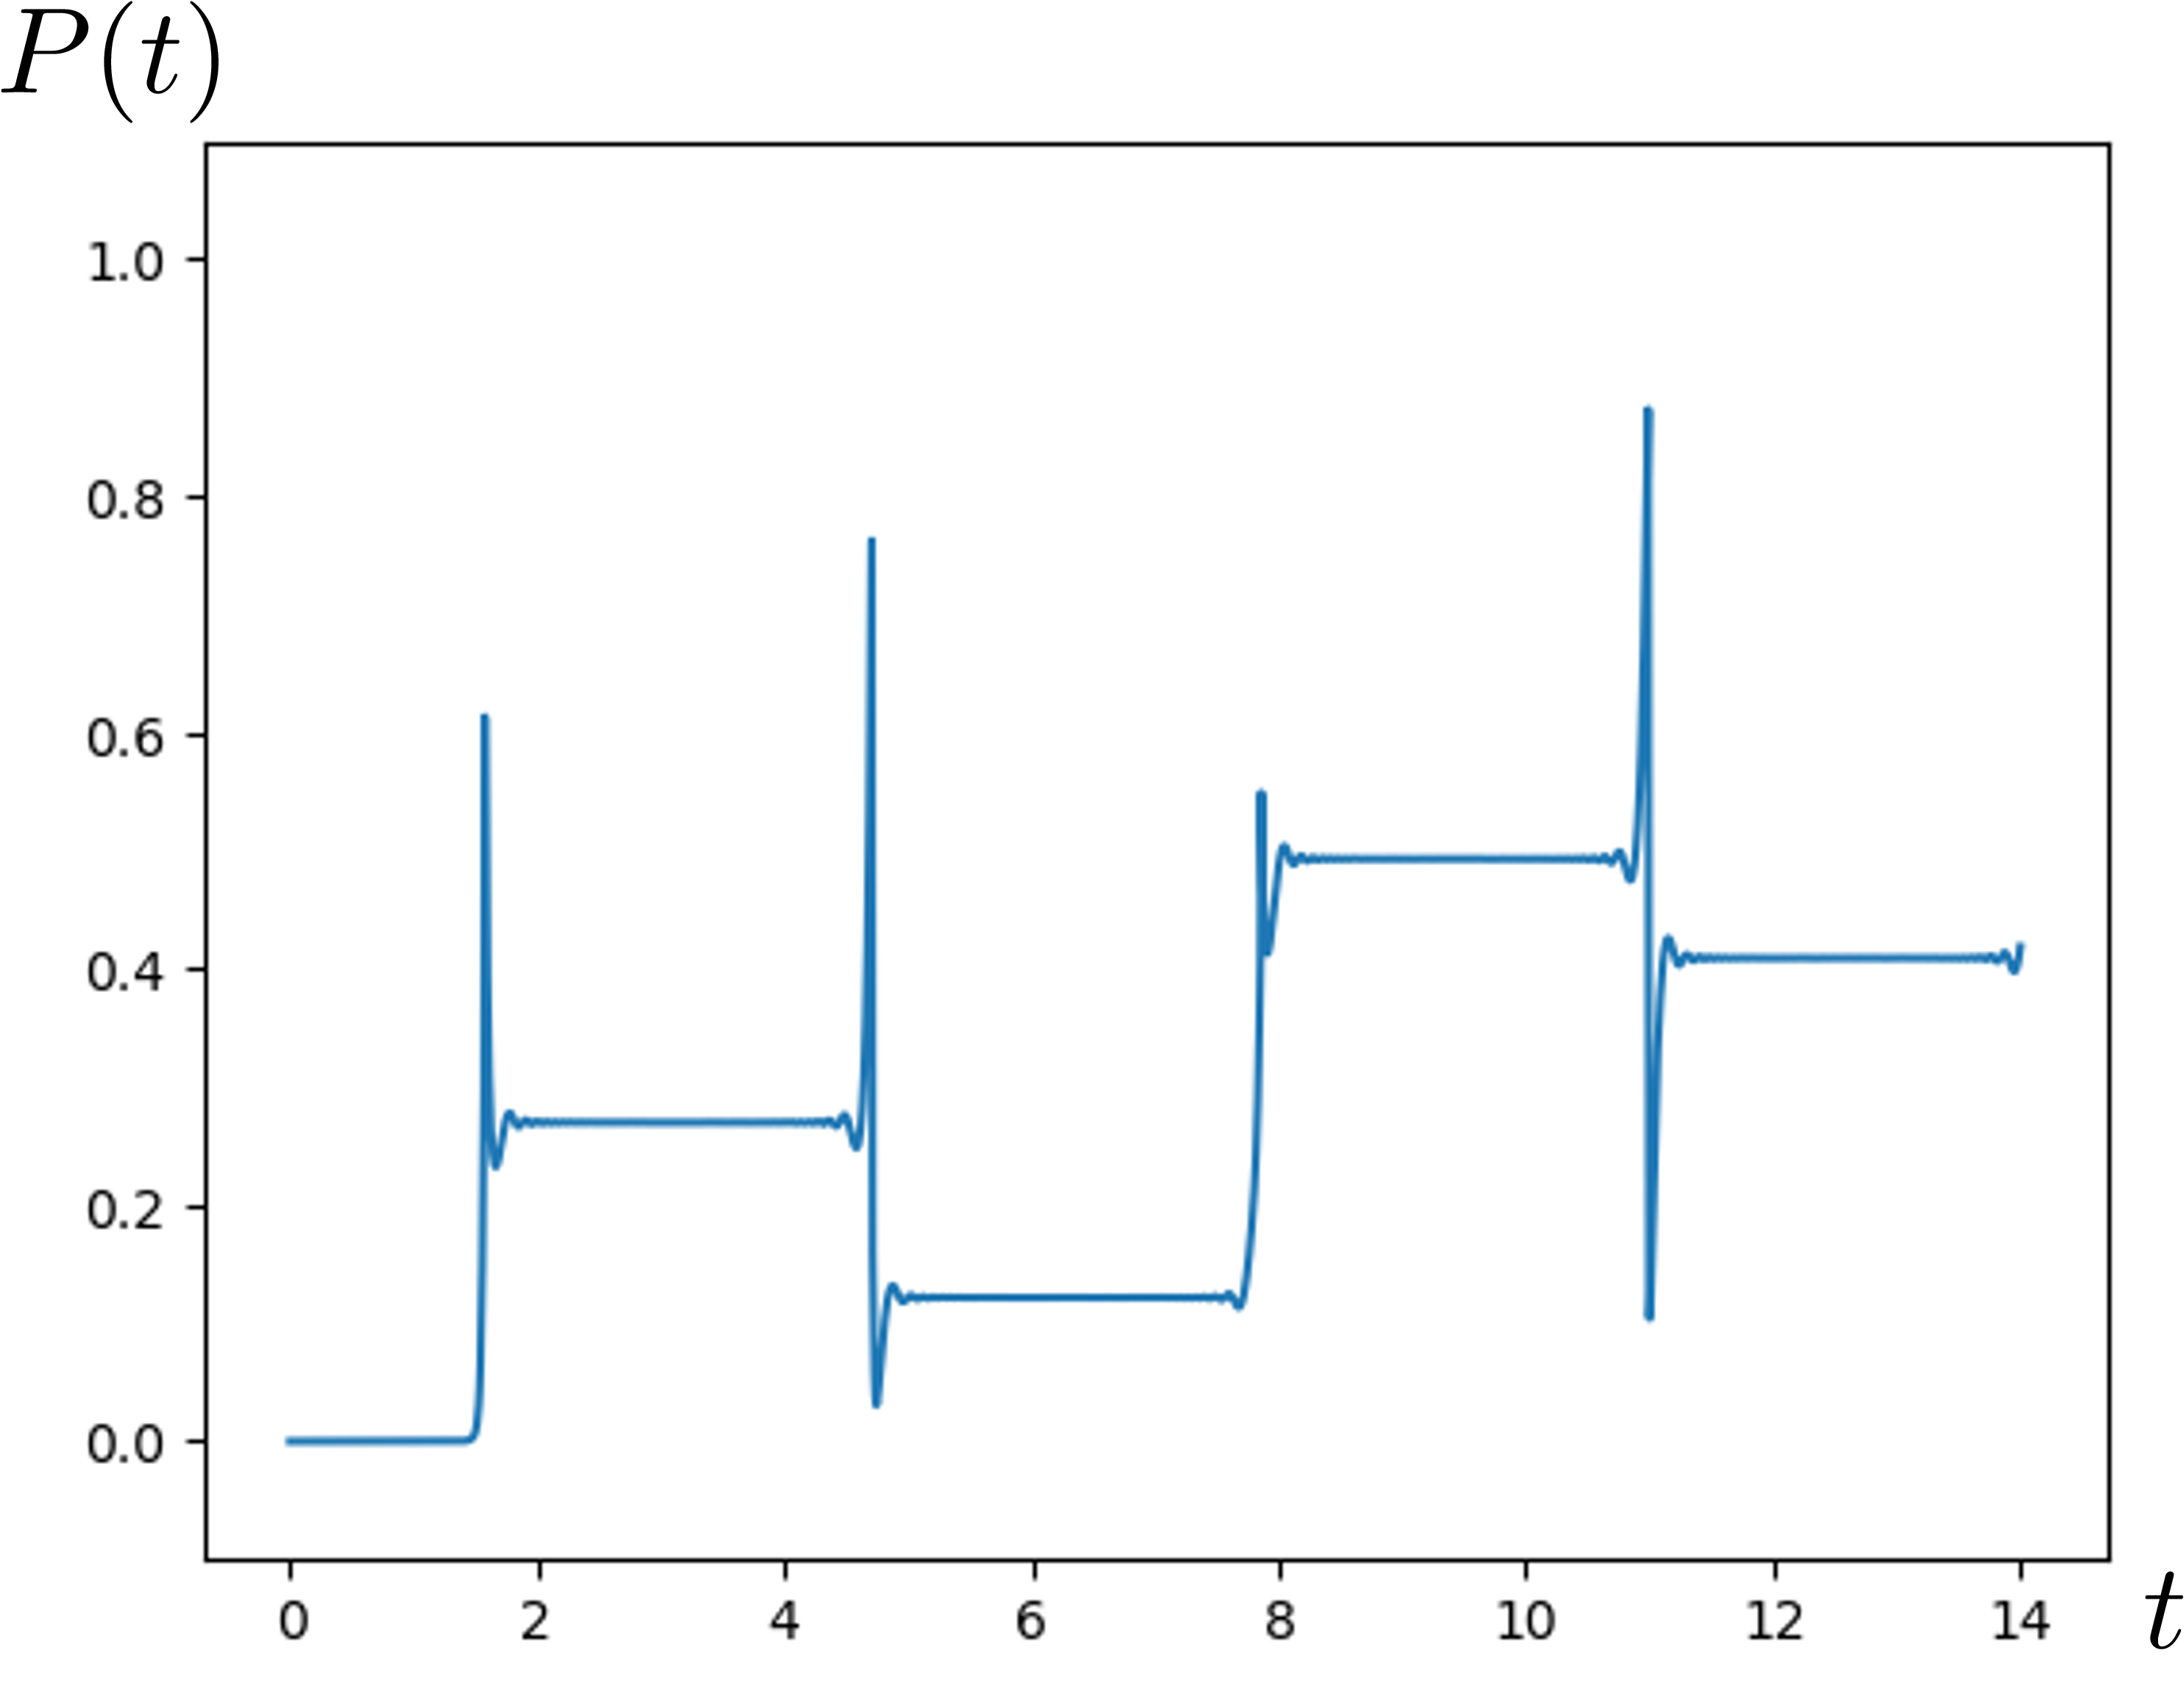
\includegraphics[scale=0.5]{figures/k_0.png}
  \caption{$\kappa_g=0$における$P(t)$の時間変化.$\varepsilon_0=90, \Delta_0 = 3, \omega=1$とした.}
  \label{fig:NR_k=0}
\end{figure}


\section{整流作用を取り入れない系}

TLZ遷移を含むcyclic evolutionで整流作用を取り入れない系のHamiltonianは
\begin{align}
  \Hat{H} = \Delta_0 \sin \omega t \, \Hat{\sigma}_x +\frac{1}{4} \kappa_g \varepsilon_0^2 \left| \cos \omega t \sin 2 \omega t \right| \, \Hat{\sigma}_y + \varepsilon_0 \cos \omega t \, \Hat{\sigma}_z \label{TLZ_CE_2}
\end{align}
である.Pauli行列を基底とした空間に,このHamiltonianを描写すると図\ref{fig:TLZ_CE2_1}から図\ref{fig:TLZ_CE2_5}のようになる.図\ref{fig:TLZ_CE_Pauli_1}から図\ref{fig:TLZ_CE_Pauli_3}とは違い,$x$軸正の向きおよび負の向きともに$y$軸正の向きに曲率が付いている.また,$\kappa_g=0.27$として,系が状態$|1\rangle$である確率($|1\rangle$ occupation probability)の時間変化をプロットすると,図\ref{fig:TLZ_CE_perfect}のようになる.完全トンネルの条件を満たすようにパラメータを設定しているため,それぞれのTLZ遷移で,常に異なる断熱状態に遷移する.したがって,有限の断熱パラメータであるにもかかわらず,この系はあたかも透熱遷移のように振る舞う.



\begin{figure}[htbp]
  \centering
  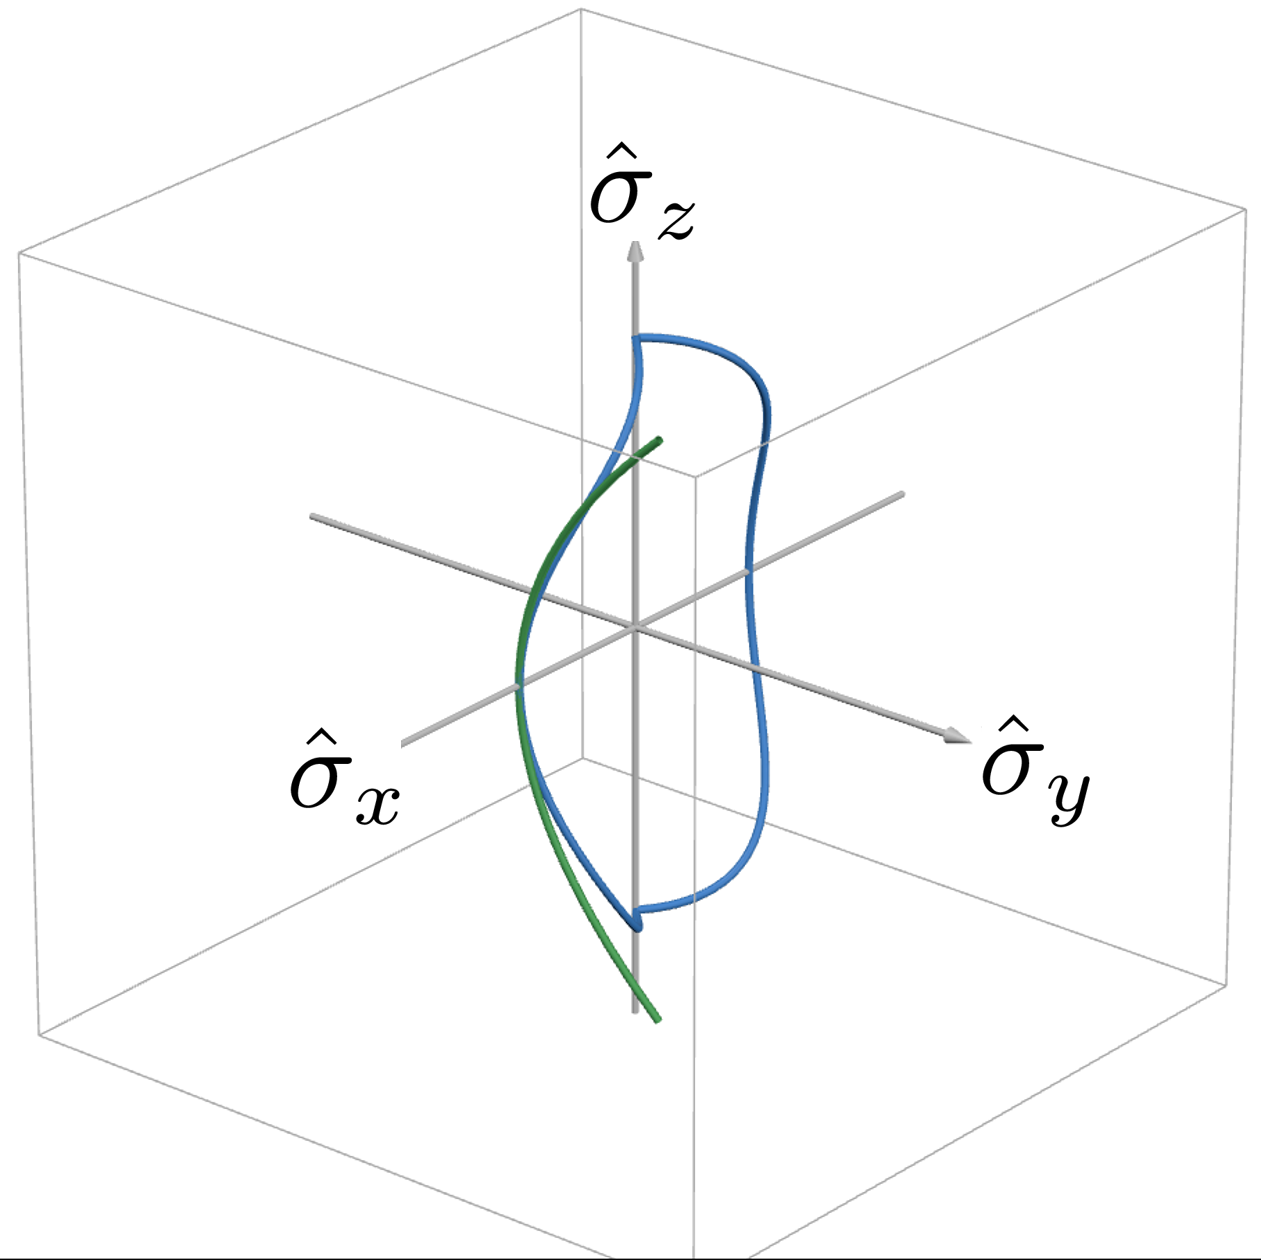
\includegraphics[scale=0.5]{figures/TLZ_CE2_1.png}
  \caption{TLZモデルを含むcyclic evolutionで整流作用を取り入れない系(\ref{TLZ_CE_2})におけるHamiltonianの経路}
  \label{fig:TLZ_CE2_1}
\end{figure}

\begin{figure}[htbp]
  \centering
  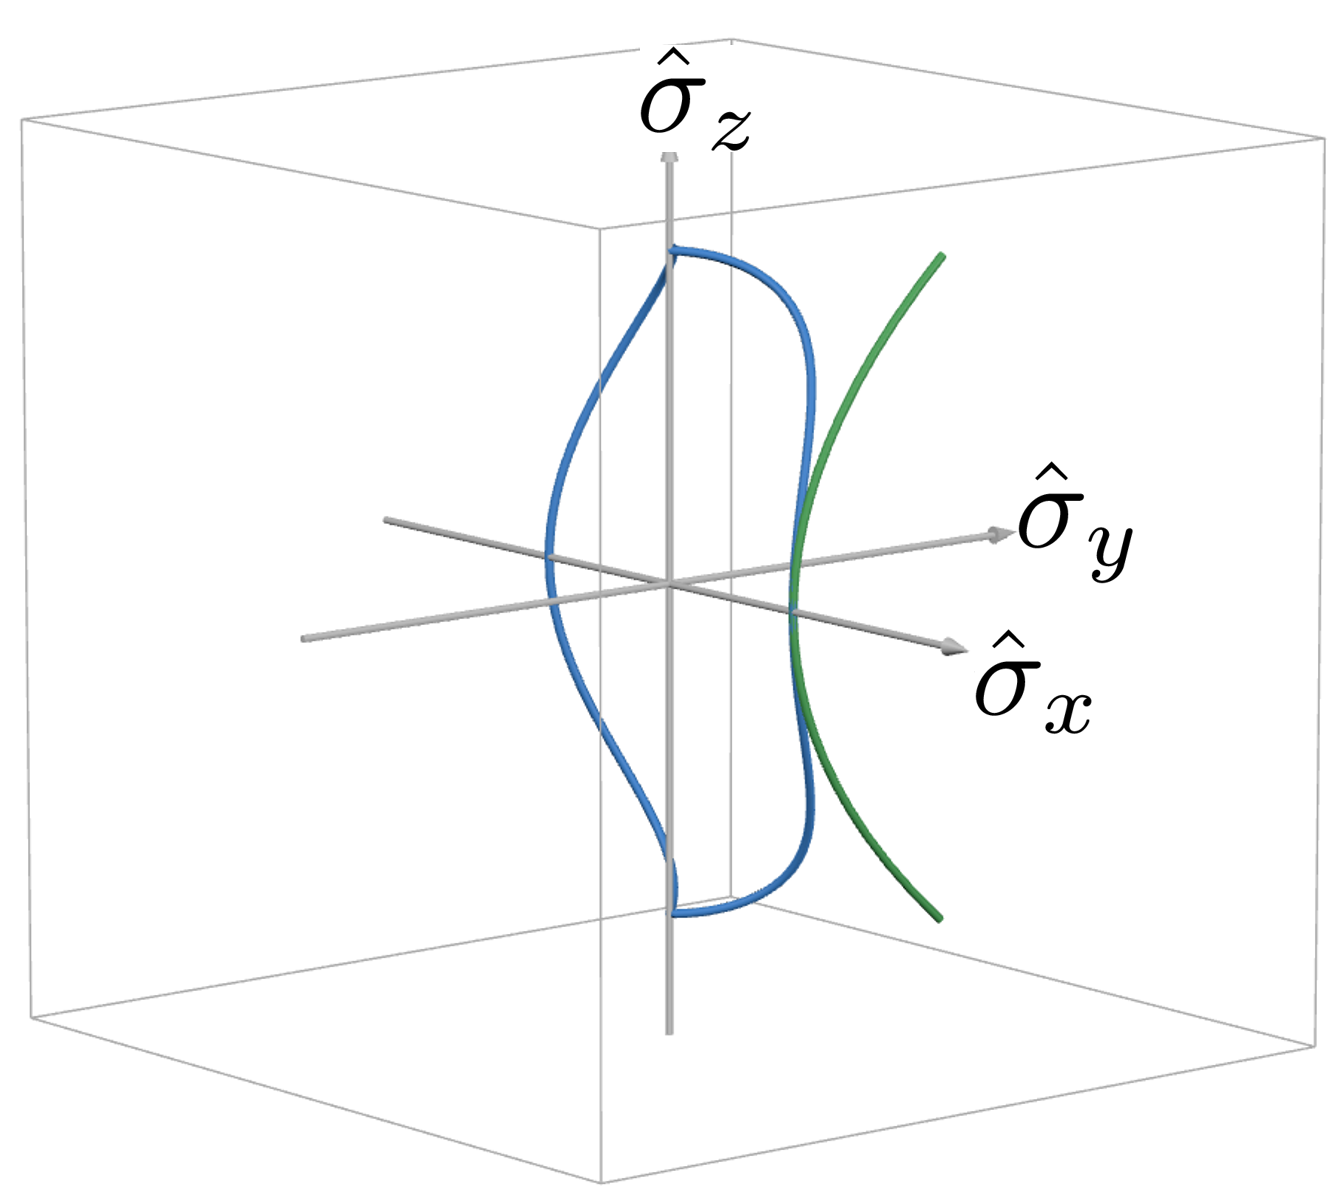
\includegraphics[scale=0.5]{figures/TLZ_CE2_2.png}
  \caption{TLZモデルを含むcyclic evolutionで整流作用を取り入れない系(\ref{TLZ_CE_2})におけるHamiltonianの経路(別の角度からの視点)}
  \label{fig:TLZ_CE2_2}
\end{figure}

\begin{figure}[htbp]
  \centering
  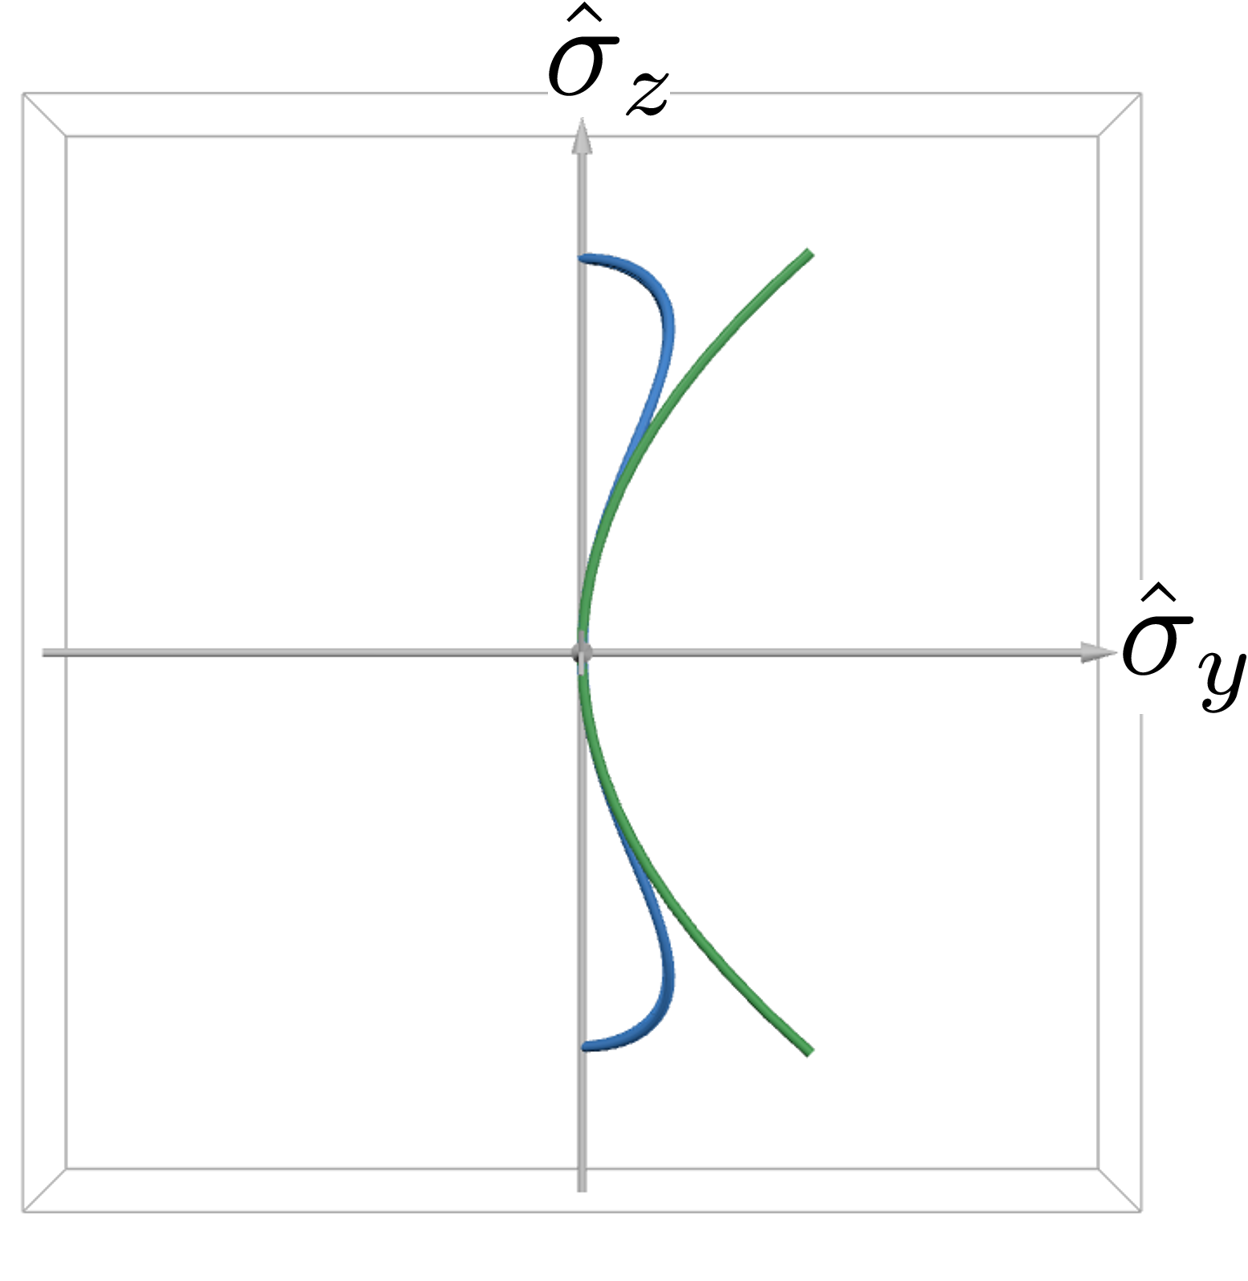
\includegraphics[scale=0.5]{figures/TLZ_CE2_3.png}
  \caption{TLZモデルを含むcyclic evolutionで整流作用を取り入れない系(\ref{TLZ_CE_2})におけるHamiltonianの経路($x$軸視点)}
  \label{fig:TLZ_CE2_3}
\end{figure}

\begin{figure}[htbp]
  \centering
  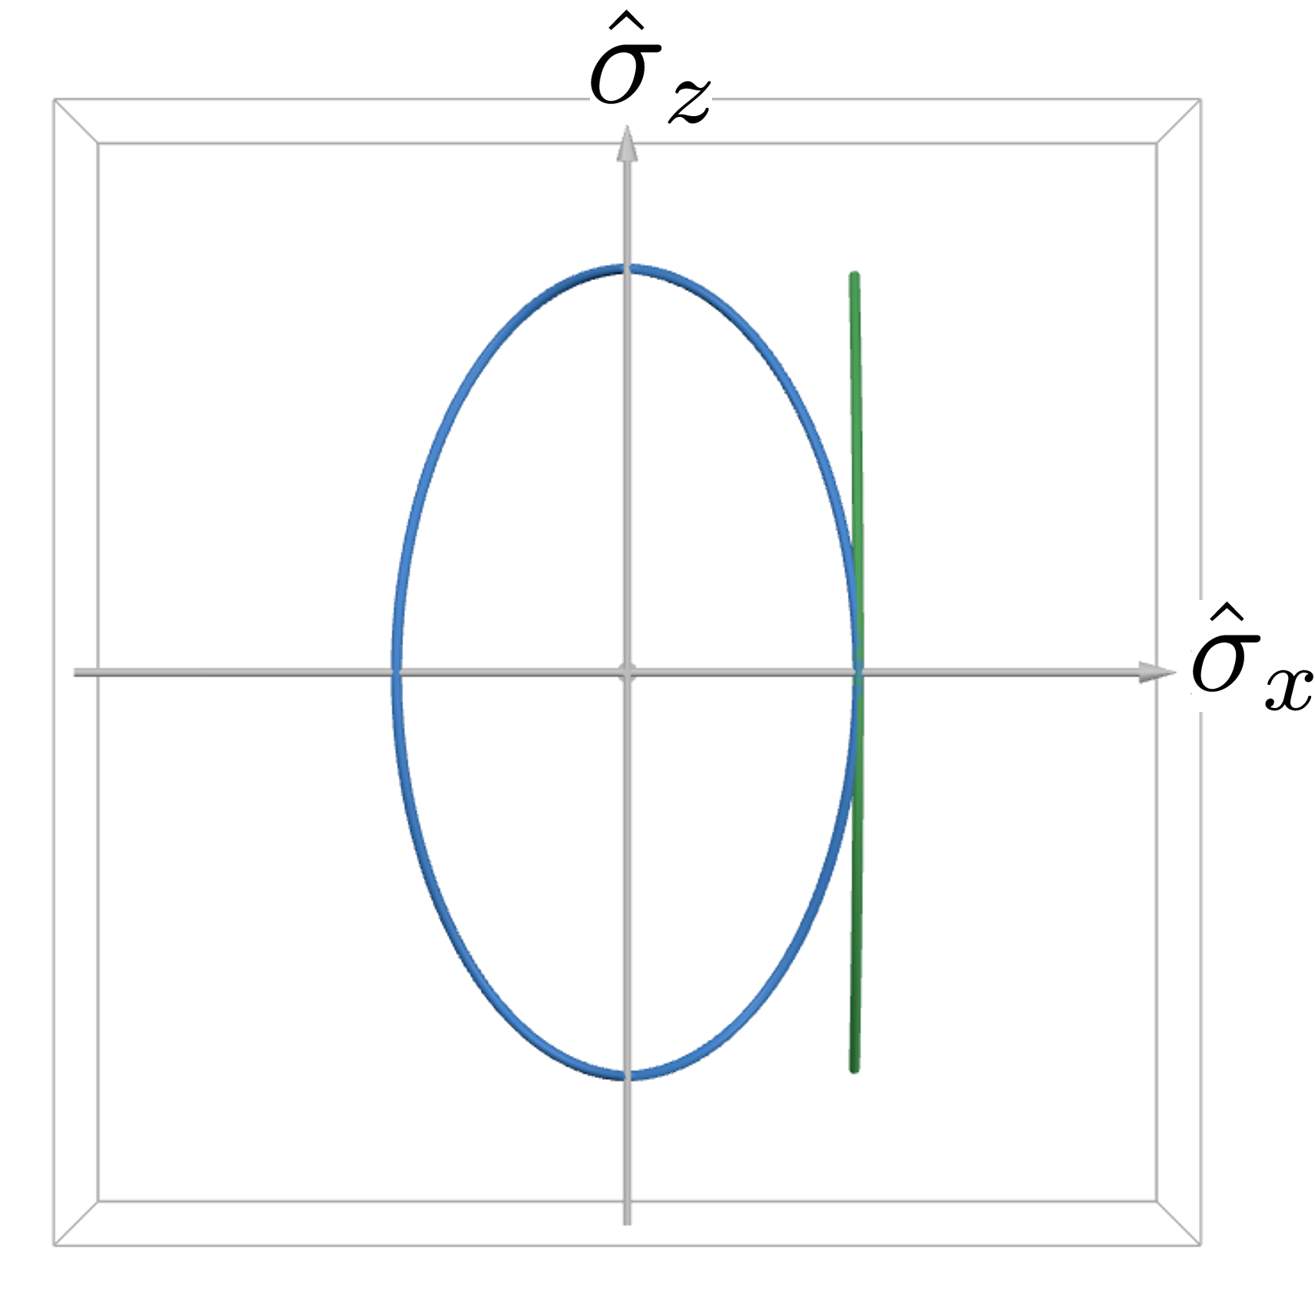
\includegraphics[scale=0.5]{figures/TLZ_CE2_4.png}
  \caption{TLZモデルを含むcyclic evolutionで整流作用を取り入れない系(\ref{TLZ_CE_2})におけるHamiltonianの経路($y$軸視点)}
  \label{fig:TLZ_CE2_4}
\end{figure}

\begin{figure}[htbp]
  \centering
  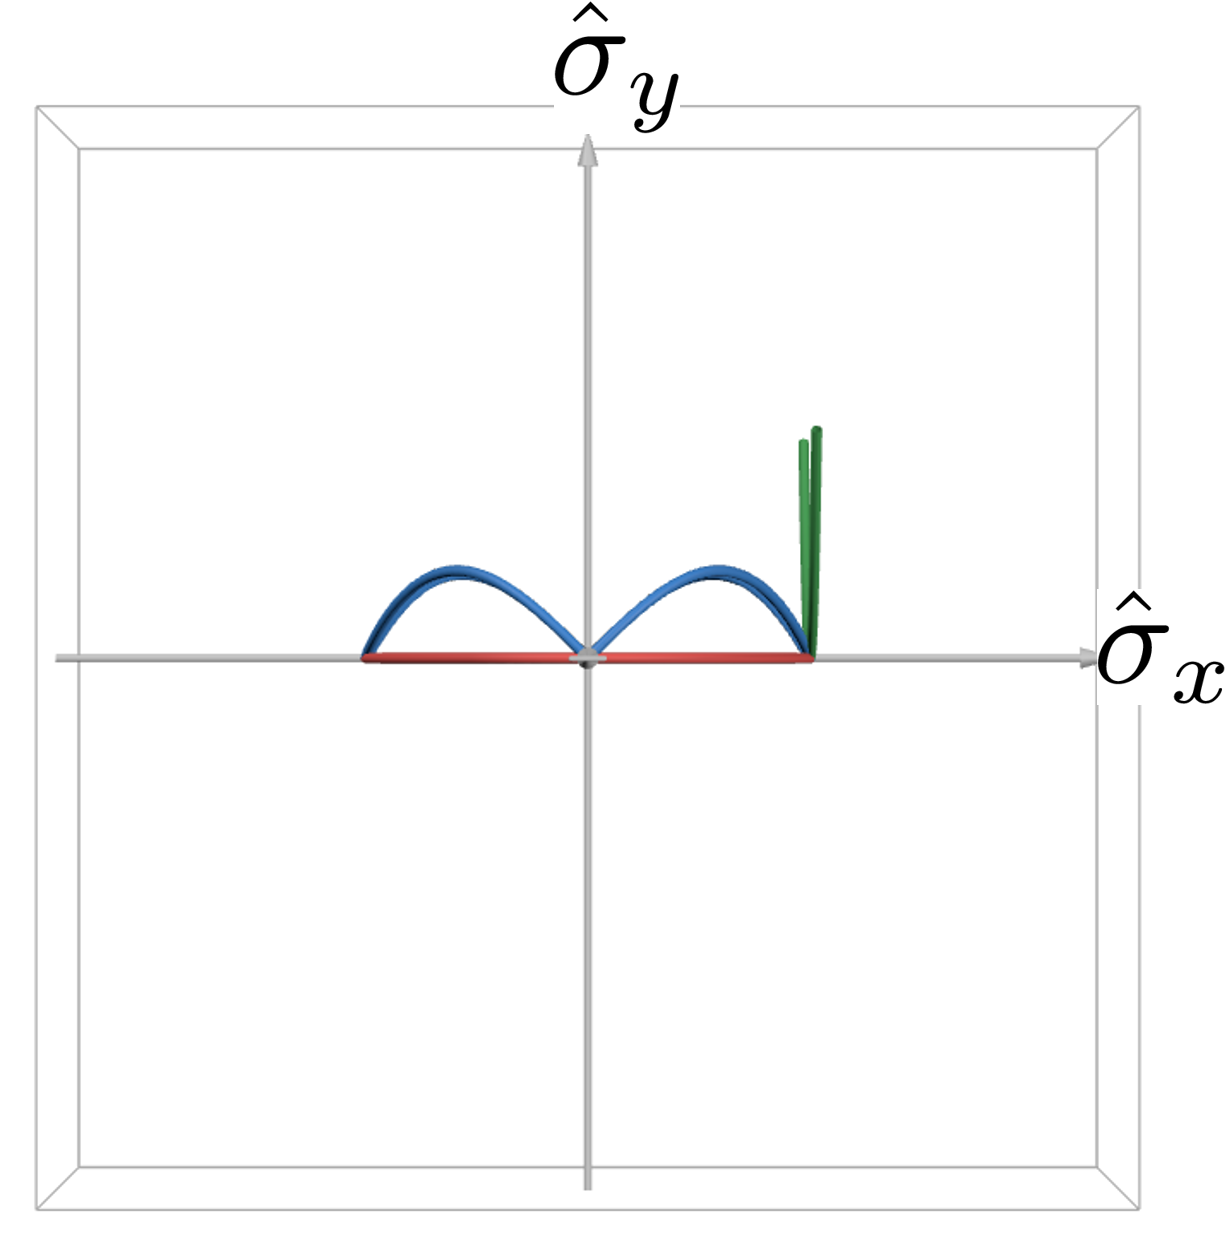
\includegraphics[scale=0.5]{figures/TLZ_CE2_5.png}
  \caption{TLZモデルを含むcyclic evolutionで整流作用を取り入れない系(\ref{TLZ_CE_2})におけるHamiltonianの経路($z$視点)}
  \label{fig:TLZ_CE2_5}
\end{figure}

\begin{figure}[htbp]
  \centering
  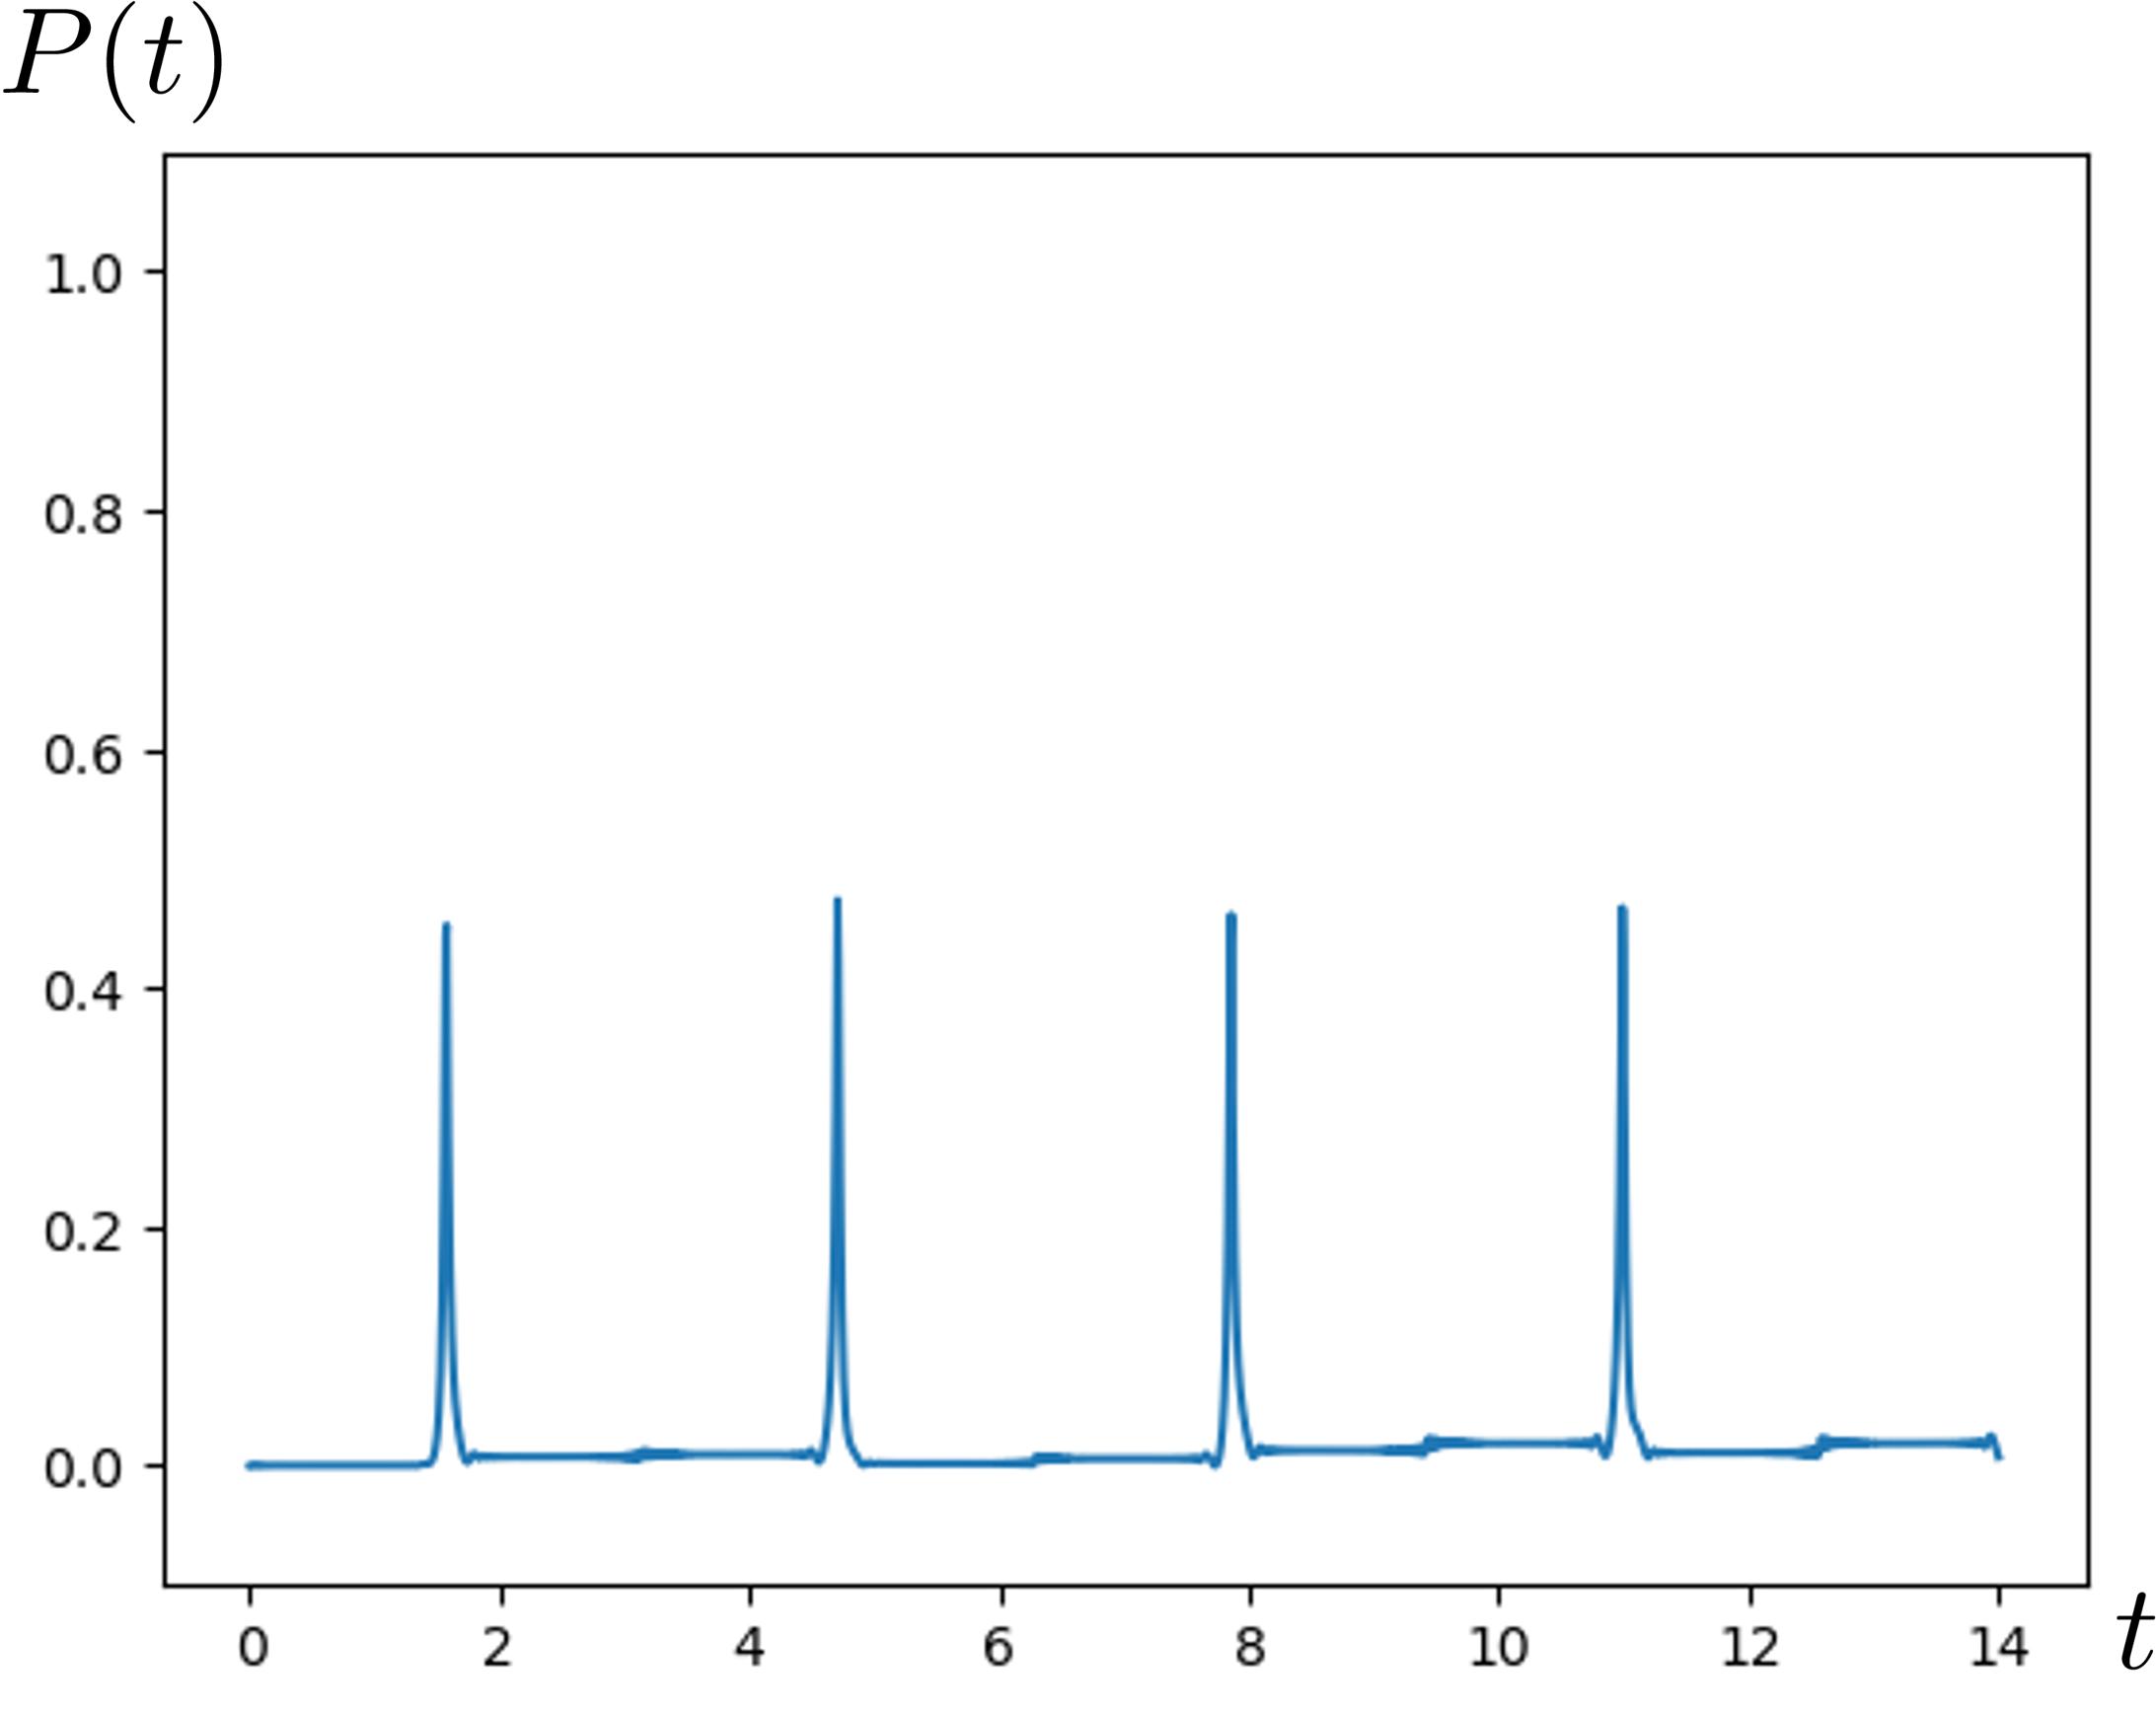
\includegraphics[scale=0.5]{figures/TLZ_CE_perfect.png}
  \caption{$\kappa_g = 0.27$のとき,TLZ遷移を含むcyclic evolutionで整流作用を取り入れない系(\ref{TLZ_CE_2})が,状態$|1\rangle$である確率.$\varepsilon_0=90, \Delta_0 = 3, \omega=1$とした.}
  \label{fig:TLZ_CE_perfect}
\end{figure}

\chapter{まとめと今後の展望}
本論文では,幾何学的な位相に注目し,Berry位相やAharonov-Anandan位相,非断熱遷移における幾何学的位相,測地曲率が,物理的な系において重要な役割を担うことを説明した.特に,Twisted Landau-Zenerモデルにおいて,測地曲率が非断熱遷移の確率に影響を与えることは,本論文のメインテーマである.また,Landau-Zenerモデルを含むcyclic evolutionという具体例を用いて,波動関数の干渉によって状態の占有確率が変化することを確認した.さらに,Twisted Landau-Zener遷移を含むcyclic evolutionを新たに考案した.そのうえで,この系において,波動関数の干渉と測地曲率が織りなす現象をみることができた.特に,完全トンネルと整流作用という測地曲率の幾何学的効果によって,2回の遷移ごとに状態の占有確率が変化する現象は,従来のcyclic evolutionでは見られない.


今後は,Twisted Landau-Zener遷移を含むcyclic evolutionにおいて,波動関数の干渉と測地曲率の関係を解析的に調べるため,波動関数の解析解を導出したい.具体的には,MajoranaやZenerがLandau-Zenerモデルに対して行った,Laplace変換や微分方程式による方法を用いて,Twisted Landau-Zenerモデルにおける波動関数の解析解の導出を模索する.仮にそれが可能であれば,転送行列法における転送行列が決定できるはずであるため,Twisted Landau-Zener遷移を含むcyclic evolutionの波動関数も導出する.また,本論文では,cyclic evolutionにおけるAharonov-Anandan位相と非断熱遷移の幾何学的位相の関係にまったく踏み込むことができなかった.Aharonov-Anandan位相は,接続の微分幾何やゲージ理論を用いて体系的に理解することができる.このように,数学的な観点から,本論文で登場したさまざまな幾何学的な量の関係を明らかにすることも今後の課題としておく.


\section*{謝辞}
非公開

\appendix
\chapter{Landau-Zener公式の証明}

\begin{equation}
  H = 
  \begin{pmatrix}
    -\frac{vt}{2} & \Delta_0\\
    \Delta_0 & \frac{vt}{2}
  \end{pmatrix}
\end{equation}
とする.また,系の状態ベクトルは,
\begin{equation}
  |\psi(t) \rangle = C_1(t) |1\rangle + C_2(t) |2\rangle
\end{equation}
である.さらに,系の初期状態は,$C_1(-\infty) = 1, C_2(-\infty) =0$としておく.このとき,Shr\"{o}dinger方程式より,
\begin{align}
  i\frac{d}{dt} C_1(t) &= -\frac{vt}{2} C_1(t) + \Delta_0 C_2(t) \label{LZ1}\\
  i\frac{d}{dt} C_2(t) &= \Delta_0 C_1(t) + \frac{vt}{2} C_2(t) \label{LZ2}\\
\end{align}
となる.式(\ref{LZ1})を微分して式(\ref{LZ2})を代入すると,
\begin{align}
  i\frac{d^2}{dt^2} C_1
  &= -\frac{v}{2} C_1(t) -\frac{vt}{2} C_1^{\prime} + \Delta_0 C_2^{\prime}\\
  &= -\frac{v}{2} C_1(t) -\frac{vt}{2} C_1^{\prime} + \Delta_0 \left( \frac{\Delta_0}{i} C_1 + \frac{vt}{2i} C_2 \right) \label{C1_A}
\end{align}
また,式(\ref{LZ2})を微分して式(\ref{LZ1})を代入すると.同様の計算から,
\begin{align}
 i\frac{d^2}{dt^2} C_2 = \frac{v}{2} C_2 + \frac{vt}{2} C_2^{\prime} + \Delta_0 \left( \frac{\Delta_0}{i} C_2 - \frac{vt}{2i} C_1 \right) \label{C2_A}
\end{align}
が得られる.したがって,式(\ref{C1_A})および式(\ref{C2_A})を整理すると,
\begin{align}
  \frac{d^2 C_1}{dt^2} + \left( \Delta_0^2 - \frac{iv}{2} \right) C_1 + \frac{v^2 t^2}{4} C_1 = 0\\
  \frac{d^2 C_2}{dt^2} + \left( \Delta_0^2 + \frac{iv}{2} \right) C_2 + \frac{v^2 t^2}{4} C_2 = 0\\
\end{align}
という$C_1$と$C_2$について独立な2つの方程式が得られる.ここで,
\begin{align}
  z &= i\sqrt{v} e^{i\frac{\pi}{4}} t \label{z_def}\\
  n &= i\delta\\
  \delta &= \frac{\Delta_0^2}{v}\\
  C_1 &= w_1(z)\\
  C_2 &= w_2(z)
\end{align}
という変数変換を行うと,
\begin{align}
  \frac{d^2 w_1}{d z^2} + \left(n + \frac{1}{2} - \frac{z^2}{4}\right) w_1 = 0\\
  \frac{d^2 C_2}{d z^2} + \left(n - \frac{1}{2} - \frac{z^2}{4}\right) w_2 = 0
\end{align}
が得られる.これらはWeberの微分方程式である.ここで,Weberの微分方程式の基本解である放物柱関数$D_n(z)$を用いて,
\begin{align}
  w_1 &\propto D_n(z)\\
  w_2 &\propto D_{n-1}(z)
\end{align}
としてよい.なぜなら,式(\ref{z_def})より,$t<0$で,
\begin{equation}
  z = i\sqrt{v} e^{i\frac{\pi}{4}} |t| = \sqrt{v} e^{-i\frac{\pi}{4}} |t|
\end{equation}
より,
\begin{equation}
  |\arg z| = \frac{\pi}{4} < \frac{3\pi}{4}
\end{equation}
であるから,放物柱関数$D_n(z)$に成り立つ定理
\begin{quote}
  $|z| \gg 1$のとき,$|\arg z| < \frac{3\pi}{4}$ならば
  \begin{equation}
    D_n(z) \rightarrow e^{-\frac{z^2}{4}} z^n
  \end{equation}
\end{quote}
を用いることができる.したがって,$t \rightarrow - \infty$で,
\begin{align}
  D_n(z) &= e^{-\frac{z^2}{4}} z^n\\
  D_{n-1}(z) &= e^{-\frac{z^2}{4}} z^{n-1}
\end{align}
と書ける.ここで,
\begin{align}
  z^n
  &= z^{i\delta}\\
  &= \exp(i\delta \log z)\\
  &= \exp(i\delta (\log \sqrt{v} e^{-\frac{i\pi}{4}} |t|))\\
  &= \exp \left( i\delta (\log (\sqrt{v} |t|) - \frac{i\pi}{4} \right)
\end{align}
より,$x \in \mathbb{R}$のとき,
\begin{align}
  D_n(z) = \exp \left( i\delta (\log (\sqrt{v} |t|) + \frac{\pi \delta}{4} \right) \label{D_n}\\
  D_{n-1}(z) = \frac{\exp \left( i\delta (\log (\sqrt{v} |t|) + \frac{\pi \delta}{4} \right)}{\sqrt{v} e^{-\frac{i\pi}{4}} |t|} \label{D_n-1}
\end{align}
であるから,$t \rightarrow -\infty$で,
\begin{align}
  |D_n(z)| &\rightarrow \text{有限}\\
  |D_{n-1}(z)| &\rightarrow 0
\end{align}
となる.これは,系の初期条件
\begin{align}
  C_1(-\infty) \ne 0\\
  C_2(-\infty) = 0
\end{align}
を満たす.したがって,任意定数$A,B$を用いて,
\begin{align}
  C_1(t) &= w_1(z) = A D_n(z),\\
  C_2(t) &= w_2(z) = B D_{n-1}(z)
\end{align}
としてよい.したがって,式(\ref{D_n})および式(\ref{D_n-1})より,$t \rightarrow -\infty$のとき,
\begin{align}
  \lim_{t \rightarrow -\infty} C_1(t) &= A \exp \left( \frac{ivt^2}{4} + \frac{\pi \delta}{4} + i\delta \log \sqrt{v} |t| \right) \label{C1_inf}\\
  \lim_{t \rightarrow -\infty} C_2(t) &= 0
\end{align}
である.


一方,$t \rightarrow \infty$のとき,
\begin{align}
  z &= \sqrt{v} e^{i\frac{3\pi}{4}},\\
  z^n
  &= z^{i\delta}\\
  &= \exp(i\delta \log z)\\
  &= \exp ( i\delta \log (\sqrt{v} t e^{i\frac{3\pi}{4}}))\\
  &= \exp \left( i\delta (\log \sqrt{v} t) + i\frac{3\pi}{4} \right)
\end{align}
となる.ここで,放物柱関数$D_n(z)$に成り立つ定理
\begin{quote}
  $\frac{\pi}{4} < \arg z < \frac{3\pi}{4}$のとき,
  \begin{equation}
    D_n(z) \rightarrow e^{-\frac{z^2}{4}} z^n - \frac{\sqrt{2\pi}}{\Gamma(-n)} e^{in\pi} e^{\frac{z^2}{4}} z^{-n-1}
  \end{equation}
\end{quote}
を用いる.このとき,$C_1(t)$については,$t \rightarrow \infty$で(第2項)$\rightarrow 0$より,
\begin{equation}
  \lim_{t\rightarrow \infty} C_1(t) = A \exp \left( \frac{ivt^2}{4} - \frac{e\pi \delta}{4} + i\delta \log (\sqrt{v}t) \right) \label{C1_lim2}
\end{equation}
となる.また,$C_2(t)$については,$t \rightarrow \infty$(第1項)$\rightarrow 0$より,
\begin{align}
  \lim_{t \rightarrow \infty} C_2(t)
  &= -B \frac{\sqrt{2 \pi}}{\Gamma(n+1)} e^{i(n-1) \pi} e^{\frac{z^2}{4}} z^{-n} \\
  &= -B \frac{\sqrt{2 \pi}}{\Gamma(1-i \delta)} \exp \left(i(i \delta-1) \pi-\frac{i v t^2}{4}-i \delta \log (\sqrt{v} t) \frac{3 \pi   \delta}{4}\right) \\
  & = B \frac{\sqrt{2 \pi}}{\Gamma(1-i \delta)} \exp \left(-\frac{\pi \delta}{4}-\frac{i v t^2}{4}-i \delta \log \sqrt{v} t\right)
\end{align}
となる.したがって,式(\ref{C1_inf})および式(\ref{C1_lim2})より,
\begin{equation}
  \frac{\lim_{t \rightarrow \infty} C_1(t)}{\lim_{t \rightarrow -\infty} C_1(t)} = \exp (-\pi \delta)
\end{equation}
であり,Landau-Zener公式
\begin{equation}
  P = \left| \frac{\lim_{t \rightarrow \infty} C_1(t)}{\lim_{t \rightarrow -\infty} C_1(t)} \right|^2  = \exp(-2\pi \delta)
\end{equation}
が示された.

\chapter{Dykhne-Davis-Pechukas法}
Shr\"{o}dinger方程式
\begin{equation}
  i\hbar \frac{d}{dt} |\psi(t) \rangle = H(t) |\psi(t) \rangle
\end{equation}
で,
\begin{align}
  |\psi(t) \rangle = a_1(t) \exp \left(-i \int_0^t d\tau \frac{E_1(\tau)}{\hbar} \right) |\phi_1(t)\rangle + a_2(t) \exp \left(-i \int_0^t d\tau \frac{E_2(\tau)}{\hbar} \right) |\phi_2(t)\rangle
\end{align}
を仮定する.ただし,$|\phi_i(t)\rangle$は断熱状態である.このとき,
\begin{align}
  a_1^{\prime} &= -\gamma \exp \left( -\frac{i\Delta}{\hbar} \right) a_2\\
  a_2^{\prime} &= \gamma \exp \left( \frac{i\Delta}{\hbar} \right) a_1
\end{align}
となる.ただし,
\begin{align}
  \gamma(t) &:= \langle \phi_1 | \phi_2^{\prime} \rangle\\
  \Delta(t) &:= \int_0^t d\tau (E_2 - E_1)
\end{align}
を定義した.ここで,$\Delta(t_c) = 0$となる$\Delta(t)$の零点$t_c$を用いて,
\begin{align}
  \tilde{a}_1 &= a_1(t)\\
  \tilde{a}_2 &= \exp \left( - \frac{i\Delta_c}{\hbar} \right) a_2(t)
\end{align}
を定義する.このとき,
\begin{align}
  \tilde{a}_1^{\prime} &= -\gamma \exp \left( \frac{-i (\Delta - \Delta_c)}{\hbar} \right) \tilde{a}_1\\
  \tilde{a}_2^{\prime} &= \gamma \exp \left( \frac{i (\Delta - \Delta_c)}{\hbar} \right) \tilde{a}_2
\end{align}
が成り立つ.ここで,図\ref{fig:Integral_path}のような複素積分区間を考える.また,$a_1(t_+)$および$a_2(t_+)$は,$a_1(t_-)$および$a_2(t_-)$から求められる.すなわち,
\begin{align}
  \begin{pmatrix}
    a_1(t_+)\\
    a_2(t_+)
  \end{pmatrix}
  =
  \begin{pmatrix}
    1_- & \Gamma_-\\
    \Gamma_+ & 1_+
  \end{pmatrix}
  \begin{pmatrix}
    a_1(t_-)\\
    a_2(t_-)
  \end{pmatrix} \label{Appendix_TM}
\end{align}
と書ける.ただし,
\begin{equation}
  \exp (\pm) := \exp \left(\pm \frac{i (\Delta - \Delta_c)}{\hbar}\right)
\end{equation}
とする.また,
\begin{align}
  1_{\pm} &= 1 - \int_{t_-}^{t_+} dt_1 \gamma \exp(\pm) \int_{t_-}^{t_1} dt_2 \gamma \exp(\mp)\\
  \Gamma_{\pm} &= \pm \int_{t_-}^{t_+} dt_1 \gamma \exp(\mp) - \int_{t_-}^{t_+} dt_1 \gamma \exp(\pm) \int_{t_-}^{t_1} dt_2 \gamma \exp(\mp) \int_{t_-}^{t_2} dt_3 \gamma \exp(\pm)
\end{align}
とする.式(\ref{Appendix_TM})に含まれる転送行列は,$\hbar \rightarrow 0$のとき,
\begin{equation}
  \begin{pmatrix}
    1_- & \Gamma_-\\
    \Gamma_+ & 1_+
  \end{pmatrix}
  \rightarrow
  \begin{pmatrix}
    1 & 0\\
    1 & 1
  \end{pmatrix}
\end{equation}
であることが知られている\cite{DavisPechukas1976}.


\begin{figure}[htbp]
  \centering
  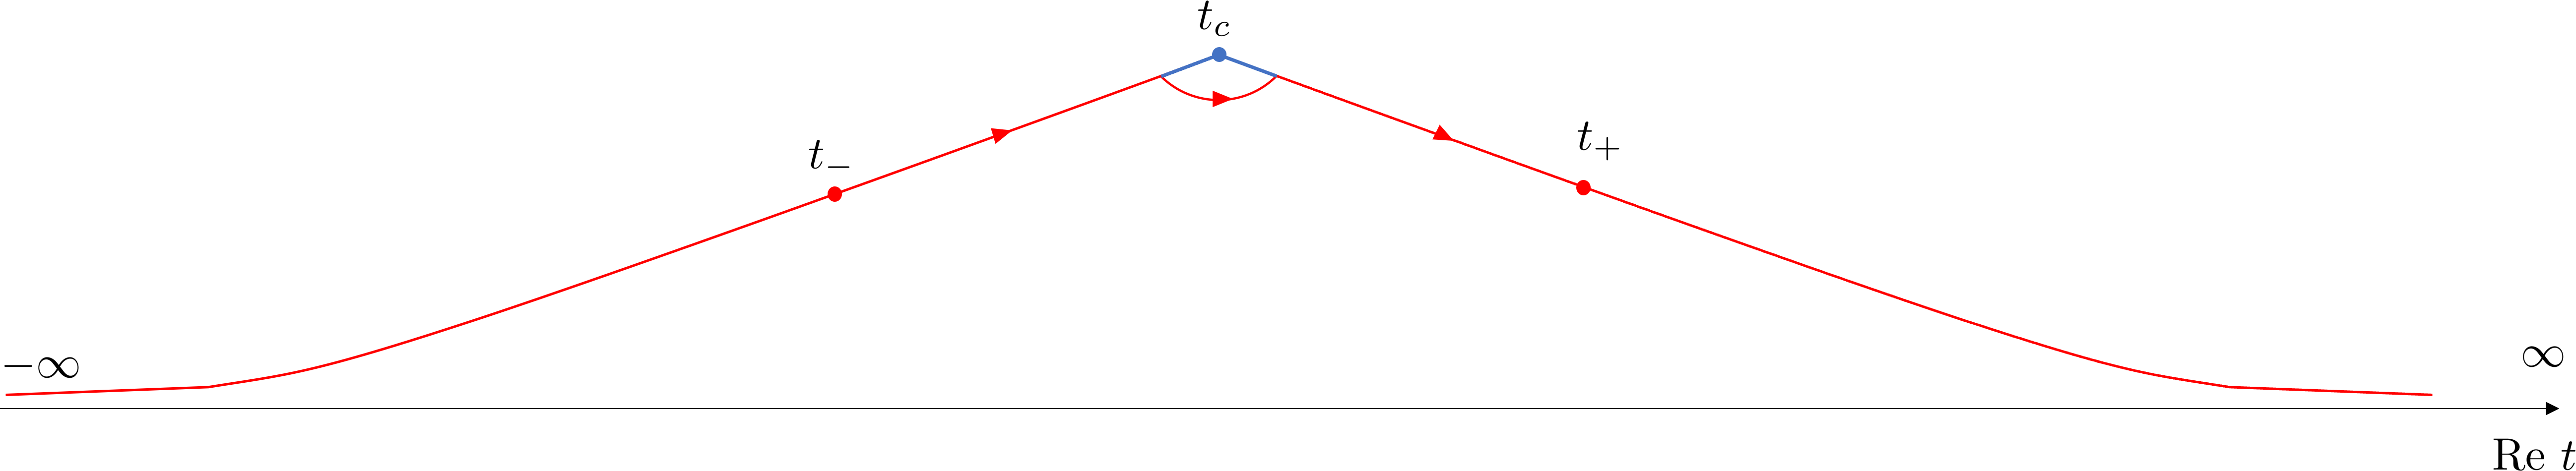
\includegraphics[scale=0.35]{figures/Integral_path.png}
  \caption{付録Bにおける複素積分の積分区間.$t_-$から$t_c$までの経路および$t_c$から$t_+$までの経路は"arm"あるいは"tail"と呼ぶ.また,$t_c$を迂回するような扇形の経路は,"center contour"と呼ぶ.}
  \label{fig:Integral_path}
\end{figure}


ここでは,特に重要な$\Gamma_+ \rightarrow 1$のみを示そう.任意の実対称Hamiltonian
\begin{equation}
  H =
  \begin{pmatrix}
    H_{11} & H_{12}\\
    H_{21} & H_{22}
  \end{pmatrix}
\end{equation}
の固有値は,
\begin{align}
  E_{\pm}
  &= \frac{H_{11} + H_{22}}{2} \pm \frac{\sqrt{(H_{11}-H_{22})^2 + 4 H_{12}^2}}{2}\\
  &:= \bar{E} \pm \frac{\delta E}{2}
\end{align}
となる.また,
\begin{align}
  H &= \bar{E} + \frac{\delta E}{2} 
  \begin{pmatrix}
    -\cos\theta & \sin \theta\\
    \sin\theta & \cos\theta
  \end{pmatrix}\\
  \tan \theta &= -\frac{2H_{12}}{H_{11}-H_{22}} \label{tan}\\
  \exp(2i\theta) &= \frac{H_{11} - H_{22} - 2i H_{12}}{H_{11} - H_{22} + 2i H_{12}} \label{exp}
\end{align}
と書ける\footnote{式(\ref{tan})と式(\ref{exp})は等価である.}.このとき,固有ベクトルは,
\begin{align}
  |\phi_1\rangle &= 
  \begin{pmatrix}
    \cos \frac{\theta}{2}\\
    -\sin \frac{\theta}{2}
  \end{pmatrix}\\
  |\phi_2\rangle &= 
  \begin{pmatrix}
    \sin \frac{\theta}{2}\\
    \cos \frac{\theta}{2}
  \end{pmatrix}\\  
\end{align}
となる.したがって,nonadiabatic coupling $\gamma$は
\begin{equation}
  \gamma = \pm \frac{\theta^{\prime}}{2} \label{gamma_B}
\end{equation}
となる.ここで,
\begin{align}
  \delta E^2
  &= (H_{11} - H_{22})^2 + 4 H_{12}^2\\
  &= (H_{11} - H_{22} + 2i H_{12})(H_{11} - H_{22} - 2i H_{12})
\end{align}
であり,$\delta E = \alpha (t - t_c)^{\frac{1}{2}}$とすると,
\begin{equation}
  (H_{11} - H_{22} + 2i H_{12}) = \frac{\alpha (t - t_c)}{H_{11} - H_{22} - 2i H_{12}}
\end{equation}
または,
\begin{equation}
  (H_{11} - H_{22} - 2i H_{12}) = \frac{\alpha (t - t_c)}{H_{11} - H_{22} + 2i H_{12}}
\end{equation}
である.したがって,
\begin{equation}
  \exp (2i\theta) = \frac{(H_{11} - H_{22} - 2i H_{12})^2}{\alpha (t - t_c)} \sim \frac{1}{\alpha (t - t_c)} \label{exp2itheta1}
\end{equation}
または,
\begin{equation}
  \exp (2i\theta) = \frac{\alpha (t - t_c)}{(H_{11} - H_{22} - 2i H_{12})^2} \sim \alpha (t - t_c) \label{exp2itheta2}
\end{equation}
より,式(\ref{exp2itheta1})と式(\ref{exp2itheta2})をまとめると,
\begin{equation}
  \exp(2i\theta) \sim (\alpha (t - t_c))^{\pm 1}
\end{equation}
と書ける.よって,
\begin{equation}
  2i\theta^{\prime} \exp(2i\theta) \sim \alpha 
\end{equation}
または,
\begin{equation}
  2i\theta^{\prime} \exp(2i\theta) -\frac{1}{\alpha (t - t_c)^2}
\end{equation}
となる.したがって,
\begin{equation}
  \theta^{\prime} \sim \frac{1}{2i} \frac{1}{t-t_c}
\end{equation}
より,式(\ref{gamma_B})に代入すると,
\begin{equation}
  \gamma \approx \frac{1}{4i} \frac{1}{t-t_c}
\end{equation}
となる.また,
\begin{align}
  \Delta(t)
  &= \int_0^t d\tau \delta E\\
  &\approx \int_0^t d\tau \alpha (t - t_c)^{\frac{1}{2}}\\
  &= \frac{2\alpha (t-t_c)^{\frac{3}{2}}}{3} - \frac{2}{3} \alpha t_c^{\frac{3}{2}}\\
  &= \frac{2\alpha (t-t_c)^{\frac{3}{2}}}{3} + \Delta(t_c)
\end{align}
である.よって,
\begin{equation}
  \gamma \exp \left(\frac{i(\Delta-\Delta_c)}{\hbar} \right) \sim \frac{1}{4i(t-t_c)} \exp \left(\frac{2\alpha (t-t_c)^{\frac{3}{2}}}{3\hbar} \right)=: L(t) \label{L_t}
\end{equation}
となる.ただし,式(\ref{L_t})の右辺を$L(t)$と置いた.このとき,
\begin{equation}
  x = \frac{2\alpha (t-t_c)^\frac{3}{2}}{3\hbar}
\end{equation}
とすると,
\begin{equation}
  \int d\tau L(t) = \int dx \frac{e^{ix}}{6ix}
\end{equation}
であることが簡単な計算からわかる.


$\tilde{a}_1(-\infty) =1$,$\tilde{a}_2(-\infty) = 0$とすると,
\begin{align}
  \tilde{a}_2(\infty)
  &\approx \tilde{a}_2(t_+)\\
  &= \int_{-\infty}^{\infty} dt \gamma \exp(+) \tilde{a}_1(t)\\
  &\approx \int_{-\infty}^{\infty} dx \frac{e^{ix}}{6ix} \tilde{a}_1(x),\\
  \tilde{a}_1(\infty)
  &= 1- \int_{-\infty}^x dx^{\prime} \frac{e^{-ix^{\prime}}}{6ix^{\prime}}  \tilde{a}_2(x^{\prime})\\
  &= 1 + \frac{1}{36} \int_{-\infty}^x dx^{\prime} \frac{e^{-ix^{\prime}}}{x^{\prime}} \int_{-\infty}^x dx^{\prime\prime} \frac{e^{ix^{\prime\prime}}}{x^{\prime\prime}} \tilde{a}_1(x^{\prime\prime})\\
\end{align}
となる.ここで,
\begin{equation}
  \tilde{a}_1(x) \sim \sum_{n=0}^{\infty} \frac{n! \alpha_n}{(ix)^n}
\end{equation}
おくと,
\begin{equation}
  \alpha_n = - \frac{1}{36 n^2} \sum_{m=0}^{n-1} \alpha_m 
\end{equation}
であることがわかる.実際,
\begin{align}
  \tilde{a}_1(x) 
  &= 1 + \frac{1}{36} \int_{-\infty}^x dx^{\prime} \frac{e^{-ix^{\prime}}}{x^{\prime}} \int_{-\infty}^{x^{\prime}} dx^{\prime\prime} \frac{e^{ix^{\prime\prime}}}{x^{\prime\prime}} \sum_{n=0}^{\infty} \frac{n! \alpha_n}{(ix^{\prime\prime})^n}\\
  &= 1+\frac{1}{36} \int_{-\infty}^x d x^{\prime} \frac{e^{-i x^{\prime}}}{x^{\prime}} \sum_{n=0}^{\infty} \frac{n! \alpha_n}{i^n} \int_{-\infty}^{x^{\prime}} d x^{\prime \prime} \frac{e^{i x^{\prime \prime}}}{\left(x^{\prime \prime}\right)^{n+1}}\\
  &= 1+\frac{1}{36} \int_{-\infty}^x d x^{\prime} \frac{e^{-i x^{\prime}}}{x^{\prime}} \sum_{n=0}^{\infty} \frac{n! \alpha_n}{i^n}\left(\left.\frac{e^{i x^{\prime \prime}}}{i (x^{\prime\prime})^{n+1}}\right|_{-\infty} ^{x^1}-\int_{-\infty}^{x^1} \frac{e^{i x^{\prime \prime}}-(n+1)}{i x^{n+2}}\right)\\
  &= 1+\frac{1}{36} \int_{-\infty}^x d x^{\prime} \frac{e^{-i x^{\prime}}}{x^{\prime}} \sum_{n=0}^{\infty} \frac{n ! \alpha_n}{i^n}\left(\frac{e^{i x^1}}{i (x^{\prime}){n+1}}+\frac{e^{i^2 x^{\prime}}(n+1)}{i\left(x^{\prime}\right)^{n+2}}+\cdots\right)\\
  &= 1+\frac{1}{36} \int_{-\infty}^x d x^{\prime} \frac{e^{-i x^{\prime}}}{x^{\prime}} \sum_{n=0}^{\infty} \sum_{k=0}^{\infty} \frac{\alpha_n(n+k) !}{\left(i x^{\prime}\right)^{n + k+1}} e^{i x^{\prime}}\\
  &= 1 + \frac{1}{36} \sum_{n=0}^{\infty} \sum_{k=0}^{\infty} \frac{\alpha_n(n+k) !}{i^{n+k+1}} \int_{-\infty}^x d x^{\prime} (x^{\prime})^{-(n+k+2)}\\
  &= 1 + \frac{1}{36} \sum_{n=0}^{\infty} \sum_{k=0}^{\infty} \frac{\alpha_n(n+k) !}{i^{n+k+1}}\left(-\frac{1}{n+k+1} x^{-(n+k+1)}\right)\\
  &= 1 + \sum_{n=0}^{\infty} \sum_{(k=0}^{\infty}\left(-\frac{1}{36}\right) \frac{\alpha_n(n+k+1) !}{(ix)^{n+k+1}(n+k+1)^2}\\
  &= 1 + \sum_{m=1}^{\infty} \sum_{k=0}^{m-1}\left(-\frac{1}{36 m^2}\right) \frac{\alpha_{m-k-1} m !}{(i x)^m}
\end{align}
より,
\begin{align}
  &\sum_{n=0}^{\infty} \frac{n ! \alpha_n}{(i x)^n} = 1+\sum_{m=1}^{\infty} \sum_{k=0}^{m-1}\left(-\frac{1}{36 m^2}\right) \frac{\alpha_k m !}{(i x)^n} \\
  \Leftrightarrow
  &1 + \sum_{n=1}^{\infty} \frac{n! \alpha_n}{(i x)^n} = 1+\sum_{m=1}^{\infty} \sum_{k=0}^{m-1}\left(-\frac{1}{36 m^2}\right) \frac{\alpha_k m !}{(i x)^m}
\end{align}
となる.ここで,あらためて$m \rightarrow n, k \rightarrow m$として,両辺を比較すると,
\begin{equation}
  \alpha_n = - \frac{1}{36 n^2} \sum_{m=0}^{n-1} \alpha_m
\end{equation}
である.では,$\alpha_n$の一般解を求めよう.そのために,
\begin{equation}
  \beta_n = -36n^2 \alpha_n \quad (n \ne 0)
\end{equation}
とすると,
\begin{align}
  \beta_{n+1}
  &= -36 (n+1)^2 \alpha_{n+1}\\
  &= \sum_{m=0}^n \alpha_m\\
  &= \alpha_n - 36n^2 \alpha_n\\
  &= \left(1-\frac{1}{36n^2} \right) \beta_n\\
\end{align}
より,
\begin{align}
  \beta_n
  &= \left(1-\frac{1}{36(n-1)^2} \right) \left( 1-\frac{1}{36(n-2)^2} \right) \cdots \left( 1-\frac{1}{36\cdot 1^2} \right) \beta_1\\
  &= \prod_{m=1}^{n-1} \left( 1-\frac{1}{36m^2} \right) 
\end{align}
となる.一方,
\begin{align}
  \tilde{a}_2(\infty) = \frac{\pi}{3} \sum_{m=0}^{\infty} \alpha_n \label{alpha_2}
\end{align}
である.実際,
\begin{align}
  \tilde{a}_2(\infty)
  &= \int_{\infty}^{\infty} dx \frac{e^{ix}}{6ix} \tilde{a}_1\\
  &= \sum_{n=0}^{\infty} \int_{\infty}^{\infty} dx \frac{n! e^{ix} \alpha_n}{6 (ix)^{n+1}}\\
  &= \sum_{n=0}^{\infty} \frac{n! \alpha_n}{6 i^{n+1}} \int_{\infty}^{\infty} dx \frac{e^{ix}}{x^{n+1}}\\
  &= \sum_{n=0}^{\infty} \frac{n! \alpha_n}{6 i^{n+1}} \left( \left. \frac{e^ix}{(-nx^n)} \right|_{\infty}^{\infty} - \int_{\infty}^{\infty} dx \frac{ie^ix}{(-nx^n)} \right)\\
  &= \sum_{n=0}^{\infty} \frac{n! \alpha_n}{6 i^{n+1}} \left( \left. \frac{e^ix}{(-nx^n)} \right|_{\infty}^{\infty} + \left. \frac{ie^{ix}}{n(-(n-1))} \right|_{\infty}^{\infty} - \int_{\infty}^{\infty} dx \frac{i^2 e^ix}{(n(-(n-1))x^{n-1}} \right) \\
  &=\sum_{n=0}^{\infty} \frac{n! \alpha_n}{6 i^{n+1}} \left( \left. \frac{i^{n-1} e^{ix}}{-n\cdots (n-(n-1))x} \right|_{\infty}^{\infty} + \int_{\infty}^{\infty} dx \frac{i^n e^{ix}}{n! x} \right)\\
  &=\sum_{n=0}^{\infty} \frac{n! \alpha_n}{6 i^{n+1}} \int_{\infty}^{\infty} dx \frac{i^n e^{ix}}{n! x}\\
  &= \sum_{n=0}^{\infty} \alpha_n \int_{\infty}^{\infty} \frac{e^{ix}}{6ix}\\
  &= \frac{\pi}{3} \sum_{m=0}^{\infty} \alpha_m
\end{align}
である.したがって,三角関数の無限積展開
\begin{equation}
  \sin (\pi z) = \pi z \prod_{n=1}^{\infty} \left( 1-\frac{z^2}{n^2} \right) \quad (z \in \mathbb{C})
\end{equation}
を用いると,
\begin{align}
  \sum_{m=0}^{\infty} \alpha_n
  &= \lim_{n \rightarrow \infty} (-36n^2 \alpha_n)\\
  &= \lim_{n \rightarrow \infty} \beta_n\\
  &= \prod_{m=1}^{\infty} \left( 1-\frac{1}{36m^2} \right)\\
  &= \frac{3}{\pi}
\end{align}
であるから,式(\ref{alpha_2})より,
\begin{equation}
  \tilde{a}_2(\infty) = 1
\end{equation}
が示された.したがって,Dykhne-Davis-Pechukas法
\begin{equation}
  a_2(\infty) \approx \exp \left( \frac{i\Delta(t_c)}{\hbar} \right)
\end{equation}
が導出された.



\begin{thebibliography}{99}
  \bibitem{Berry1984}  M. V. Berry, Proc. R. Soc. Lond. A {\bf 392}, 45 (1984).
  \bibitem{Zener} C. Zener, Proc. R. Soc. Lond. A {\bf 137}, 696 (1932).
  \bibitem{Kayanuma1993} Y. Kayanuma, Phys. Rev. B {\bf 47}, 9940 (1993).
  \bibitem{Berry1990} M. V. Berry, Proc. R. Soc. Lond. A {\bf 430}, 405 (1990).
  \bibitem{Oka} S. Takayoshi, J. Wu and T. Oka, SciPost Phys. {\bf 11}, 075 (2021).
  \bibitem{Dykhne} A. M. Dykhne, Sov. Phys. JETP {\bf 14}, 941 (1962).
  \bibitem{DavisPechukas1976} J. P. Davis and P. Pechukas, J. Chem. Phys. {\bf 64}, 3129 (1976).
  \bibitem{Hwang} J. -T. Hwang and P. Pechukas, J. Chem. Phys. {\bf 67}, 4640-4653 (1977).
  \bibitem{Wu2008} J.-d. Wu, M.-s. Zhao, J.-l. Chen and Y.-d. Zhang, Phys. Rev. A {\bf 77}, 062114 (2008).
  \bibitem{Ivakhnenko} O.V. Ivakhnenko, S.N. Shevchenko and F. Nori, Phys. Rep. {\bf 995}, 1–131 (2023).
  \bibitem{Aharonov} Y. Aharonov and J. Anandan, Phys. Rev. Lett. {\bf 58}, 1593 (1987).
  \bibitem{Kayanuma1994} Y. Kayanuma, Phys. Rev. A {\bf 50}, 843 (1994).
  \bibitem{Kayanuma1997} Y. Kayanuma, Phys. Rev. A {\bf 55}, 2495 (1997).
\end{thebibliography}

\end{document}



